%%%%%%%%%%%%%%%%%%%%%%%%%%%%%%%%%%%%%%%%%%%%%%%%%%%%%%%%%%%%%%%%%%%%%%%%%%%%%%%%%%%%%%%%%%%%%%%%%%%%%
%
%   Version     : 1.0
%
%   Filename    : main.tex
%
%   Description : 
%           
%   Author      : Briane Paul V. Samson
%
%%%%%%%%%%%%%%%%%%%%%%%%%%%%%%%%%%%%%%%%%%%%%%%%%%%%%%%%%%%%%%%%%%%%%%%%%%%%%%%%%%%%%%%%%%%%%%%%%%%%%%

%%%%%%%%%%%%%%%%%%%%%%%%%%%%%%%%%%%%%%%%%%%%%%%%%%%%%%%%%%%%%%%%%%%%%%%%%%%%%%%%%%%%%%%%%%%%%%%%%%%%%%%%%%%%%%%%%%%%%%%
%
%  Filename   : preamble.tex
%
%  Description: Preamble file to :
%               a. specify related packages
%               b. set margins, commands, etc.
%
%  Note       : Edit the margin settings for your own printer
%               You may add your own commands, environments (it is assumed that you know what you're doing.)
%
%%%%%%%%%%%%%%%%%%%%%%%%%%%%%%%%%%%%%%%%%%%%%%%%%%%%%%%%%%%%%%%%%%%%%%%%%%%%%%%%%%%%%%%%%%%%%%%%%%%%%%%%%%%%%%%%%%%%%%%

\documentclass[12pt,titlepage,onepage, letterpaper]{article}

%
%-- specify related packages
%
%\usepackage[utf8x]{inputenc}

\usepackage{apacite}           %-- APA style citation 
                               %-- refer to http://www.ctan.org/tex-archive/biblio/bibtex/contrib/apacite/
%\usepackage{ucs}

\usepackage{amsmath}           %-- American Math Society packages
\usepackage{amsfonts}
\usepackage{amssymb}

\usepackage{graphicx}          %-- graphicx package needed for including figures in EPS (Encapsulated Postcript     
\usepackage{graphics}          %-- graphics related package

\usepackage{verbatim}          %-- this package allows you to have multiple lines of comments by
                               %-- example:
                               %   \begin{comment}
                               %        ...your text here...
                               %   \end{comment}  

\usepackage{color}             %-- allows use of color with text
                               %-- example:  \textcolor{red}{This is the colored text in red.}
                               
\usepackage[english]{babel}

\usepackage{multirow}
\usepackage{float}
\floatstyle{plaintop}
\restylefloat{table}

\usepackage{alltt}
\renewcommand{\ttdefault}{txtt}

\usepackage{rotating}

\usepackage{multicol}

%
%-- set margins,  you may need to edit this for your own printer
%
\topmargin 0.0in
\oddsidemargin 0.0in
\evensidemargin 0.0in

\voffset 0.0in
\hoffset 0.5625in

\textwidth 5.75in
\textheight 8.5in


\parskip 1em
\parindent 0.25in

\bibliographystyle{apacite}            %-- use APA citation scheme

\hyphenation{ana-lysis know-ledge}     %-- LaTeX may not hyphenate correctly some words you use in your document
                                       %-- use \hyphenation to instruct LaTeX how to do it correctly, example above

\newcommand{\degree}{^{\circ}}         %-- use \newcommand to create your own "commands"
                                       %-- \newcommand works like the #define you learned in your COMPRO1 class

\newcommand{\etal}{et al.}


%\newcommand{\sinag}{\emph{Sinag}}
%\newcommand{\sinagtwo}{\emph{Sinag2}}

\newcommand{\figref}[1]{Figure \ref{#1}}
\newcommand{\appref}[1]{Appendix \ref{#1}}

\newcommand{\Section}[1]{\section{#1}\setcounter{figure}{0}\setcounter{table}{0}}

%\newcommand{\shade}{\multicolumn{1}{|>{\columncolor[gray]{0.25}}c|}{}}
%\newcommand{\tableheader}[1]{\rowcolor{black}\color{white}{#1}}
%\newcommand{\cell}[2]{\multicolumn{1}{#1}{#2}}
%\newcommand{\definition}[2]{\textbf{\textit{#1}} --- #2}
%\newcommand{\itembit}[1]{\item \textbf{\textit{#1}}}
%\newcommand{\sgdef}[2]{\parbox[t][][t]{1.75in}{\textbf{#1}} \> \parbox[t][][t]{4.0in}{#2}\\\\}

%\newenvironment{sinagglossary}{\begin{flushleft}
%\begin{tabbing}
%\hspace{1.75in}\=\\}{\end{tabbing}\end{flushleft}}

\newcommand{\thestitle}[1]{{\Large \textsc{#1}}}

\renewcommand{\thefigure}{\thesection.\arabic{figure}}
\renewcommand{\thetable}{\thesection.\arabic{table}}
\renewcommand{\contentsname}{Table of Contents}




                %-- includes LaTeX source file for the preamble 
                                  %-- include packages, sets the margin sequence, and many more... 
                                  %-- your job: check if the settings are suitable for your own printer

\begin{document}

%%%%%%%%%%%%%%%%%%%%%%%%%%%%%%%%%%%%%%%%%%%%%%%%%%%%%%%%%%%%%%%%%%%%%%%%%%%%%%%%%%%%%%%%%%%%%%%%%%%%%%
%
%   Filename    : title_page.tex 
%
%   Description : This file will contain your Title Page.
%                 
%%%%%%%%%%%%%%%%%%%%%%%%%%%%%%%%%%%%%%%%%%%%%%%%%%%%%%%%%%%%%%%%%%%%%%%%%%%%%%%%%%%%%%%%%%%%%%%%%%%%%%

\begin{titlepage}
\centering


%-- **EDIT** the following line to indicate your thesis title
\thestitle{Automatic Extraction of Conceptual Relations from Children's Stories}

\vspace{1.75cm}
A Thesis Proposal\\
Presented to\\
the Faculty of the College of Computer Studies\\
De La Salle University Manila

\vspace{1.75cm}
In Partial Fulfillment\\
of the Requirements for the Degree of\\

Master of Science in Computer Science

\vspace{1.75cm}
by\\
%-- **EDIT** the following line to indicate your name 
\vspace{1cm}

SAMSON, Briane Paul V.  \\

\vspace{1.75cm}
%-- **EDIT** the following line to indicate your adviser's name 
Ethel ONG \\
Adviser

\vspace{1.75cm}
\today
\end{titlepage}
              %-- includes LaTeX source file for the Title Page 
                                  %-- your job: **EDIT THIS FILE ** to indicate your own title, name, and thesis adviser's name

%%%%%%%%%%%%%%%%%%%%%%%%%%%%%%%%%%%%%%%%%%%%%%%%%%%%%%%%%%%%%%%%%%%%%%%%%%%%%%%%%%%%%%%%%%%%%%%%%%%%%%
%
%   Filename    : abstract.tex 
%
%   Description : This file will contain your Research Description.
%                 
%%%%%%%%%%%%%%%%%%%%%%%%%%%%%%%%%%%%%%%%%%%%%%%%%%%%%%%%%%%%%%%%%%%%%%%%%%%%%%%%%%%%%%%%%%%%%%%%%%%%%%

\begin{abstract}
People use storytelling as a natural and familiar means of conveying information and experience to each other. During this interchange, people understand each other because we rely on a large body of shared common sense knowledge. But computers do not share this knowledge, causing a barrier in human-computer interaction and in applications requiring computers to generate coherent text. To support this task, computers must be provided with a usable knowledge about the basic relationships between concepts that we find everyday in our world. 

Picture Books is a story generation system that generates stories for children age 4 to 6. To achieve this, it uses a semantic ontology containing conceptual knowledge about objects, activities and their relationships in a child's daily life. But the task of building this knowledge base is tedious and time consuming, thus limiting the variants of stories and themes that Picture Books is able to generate. This research involves the development of a software tool that will automatically extract concepts and their relations from existing children's stories, and store these in a knowledge base that Picture Books and other NLP applications can utilize to do their tasks.  

\begin{flushleft}
\begin{tabular}{lp{4.25in}}
\hspace{-0.5em}\textbf{Keywords:}\hspace{0.25em} & language parsing and understanding, text analysis, semantic networks, natural language processing  \\
\end{tabular}
\end{flushleft}
\end{abstract}
                %-- this is the Abstract page
                                  %-- your job: **EDIT THIS FILE** to indicate your own abstract

\pagenumbering{roman}             %-- this will number pages as i, ii, iii, etc...
\setcounter{page}{2}

\tableofcontents                  %-- this command is used to generate the Table of Contents

\newpage
\listoffigures                    %-- this command is used to generate List of Figures

\newpage                       
\listoftables                     %-- this command is used to generate List of Tables

\newpage

\pagenumbering{arabic}            %-- this will number pages as 1, 2, 3, etc...
\setcounter{page}{1}              

%%%%%%%%%%%%%%%%%%%%%%%%%%%%%%%%%%%%%%%%%%%%%%%%%%%%%%%%%%%%%%%%%%%%%%%%%%%%%%%%%%%%%%%%%%%%%%%%%%%%%%
%
%   Filename    : chapter_1.tex 
%
%   Description : This file will contain your Research Description.
%                 
%%%%%%%%%%%%%%%%%%%%%%%%%%%%%%%%%%%%%%%%%%%%%%%%%%%%%%%%%%%%%%%%%%%%%%%%%%%%%%%%%%%%%%%%%%%%%%%%%%%%%%


\Section{Research Description}
\label{sec:researchdesc}    %--note: labels help you with hyperlink editing (using your IDE)

This chapter discusses an overview of the current state of technology, the research objectives, scope and limitations, and its significance.

\subsection{Overview of the Current State of Technology}
\label{sec:overview}

Natural language processing systems use a set of knowledge base in order to do tasks such as text generation. But simple lexicons and large unstructured corpora may be insufficient as knowledge base of these systems. Storytelling, for instance, is a natural task for humans. Armed with a library of words, their meanings and their relationships, we combine words and events to tell stories about ourselves, our community, and our experiences. Thus computers must be provided with the same shared collection of common sense knowledge about the basic relationships between things and events that nearly every person knows in order for them to achieve a level of expressiveness same as humans and be able to understand the world that we talk about. Such knowledge are represented as conceptual relations defining the relationship between two or more concepts in real life.

Recent creative text generation systems such as \cite{Hong:2009} have utilized a semantic network representation of concepts on common sense knowledge to identify relationships of words in human puns in order to generate computer puns. Another system, Picture Books \cite{Solis:2009}, generates stories with morals for children ages 4 to 6, by using a semantic ontology, patterned after ConceptNet \cite{Liu:2004a}, containing conceptual knowledge about objects, activities, and their relationships in a child's daily life. The process of building and populating the Picture Books ontology required a lot of manual effort on the part of the proponents. Currently, the ontology contains 240 concepts and 369 relations, which were populated based on the themes that have been identified as relevant for the target age group.

Early Information Extraction (IE) systems have addressed the extraction of information from relatively small collections of well-structured documents such as newswire or scientific publications \cite{Muslea:1999}. More recently, IE systems are focused on extracting facts from structured and unstructured documents for a particular domain, such as legal documents \cite{Cheng:2008}.

Although IE systems are capable of recognizing entities within documents (e.g. `Renoir' is a `Person', `25 Feb 1841' is a `Date'), the relation between the entities (e.g., `Renoir' was born on `25 Feb 1841') is not extracted, thus generating incomplete information that may be needed by certain applications \cite{Banko:2008}. A variant of IE, Relation Extraction (RE), is the task of recognizing the assertion of a particular relationship between two or more entities in text.

The task of relation extraction is difficult, but relations such as hypernymy (IsA) and meronymy (PartOf) are often expressed using a small number of lexico-syntactic patterns \cite{Hearst:1992}. Using a sample set of 500 sentences selected at random from an IE training corpus, \citeA{Banko:2008} showed that many binary relationships are also consistently expressed using a compact set of relation-independent lexico-syntactic patterns.

The Artequakt project \cite{Alani:2003} also showed that it is possible to automatically acquire such relations from documents to populate an ontology. Working in the domain of artists, the Artequakt project identifies relations between entities of interest within sentences, following ontology relation declarations and lexical information. These relations are then used to populate an ontology with knowledge triples for use in the generation of biographies of artists.

To convey the ideas of a story, \citeA{Nakasone:2006} developed a storytelling ontology model by identifying relations between sentences in the story using the Rhetorical Structure Theory (RST) of \citeA{Mann:1987}. As \citeA{Knott:1994} pointed out, explicit and implicit relations hold between the sentences of a text, so that the content of one sentence might provide justification, elaboration or explanation for the content of another. These relations bind a text together to contribute to the overall comprehension of a story by the readers; for instance, whether understanding one text span (scene of a story) increases the reader's readiness to understand another scene, or whether understanding both spans allows the reader to recognize a particular semantic relation as holding between them. Certain discourse relations or cue phrases, such as ``but", ``so", ``although", ``more precisely" or ``for example", are used to signal explicit relations between text spans.

Although both IE and RE have achieved significant progress in extracting facts and concepts in the domains of newspapers \cite{Muslea:1999}, biographies \cite{Alani:2003}, and legal documents \cite{Cheng:2008}, limited work has been done on children's stories. Furthermore, since stories contain sequences of actions that characters perform or experience at various points in the story world, knowledge about how these events are ordered and the constraints under which they can occur must also be extracted.

\subsection{Research Objectives}
\label{sec:researchobjectives}

\subsubsection{General Objective}
\label{sec:generalobjective}

To develop a methodology that automatically identifies and extracts the relations between everyday concepts and objects from children's stories and store them in a semantic network to provide ontological knowledge for Picture Books.

\subsubsection{Specific Objectives}
\label{sec:specificobjectives}

\begin{enumerate}
   \item To collect a corpus of children's stories;
   \item To analyze the English sentence structures in the corpus;
   \item To derive a set of extraction patterns;
   \item To develop a representation for modelling relations of every object common in children's stories;
   \item To implement extraction rules using GATE for extracting conceptual relations automatically from the corpus, and;
   \item To validate the resulting conceptual relations extraction tool through integration with Picture Books
\end{enumerate}

\subsection{Scope and Limitations of the Research}
\label{sec:scopelimitations}

At least 30 children's stories were collected to form the input corpus for the extraction tool to be developed. These were then be modified to remove the dialogues. Analysis of the English sentence structures in these stories were performed to identify the types of relations that are present. This information were used to derive a set of patterns or templates for extracting conceptual relations. An extraction tool was used to use the extraction patterns to automatically locate instances of a known relation in the corpus.

One relation may be expressed in various ways in text. Consider the hypernymy (IsA) relation, wherein the following sentences are possible ways of expressing it:

	\noindent
	\hspace{1 in}\emph{The dog is a canine.} \\
	\hspace*{1 in}\emph{The dog is a kind of canine.} \\
	\hspace*{1 in}\emph{The dog, a canine, is �} \\
	\hspace*{1 in}\emph{The dog is a type of canine.}

Although lexico-syntactic extraction patterns mapped directly to relations, certain English sentence constructs require further analysis and decomposition in order to derive their corresponding relations. These include sentence structures containing conjunctions and embedded clauses, as shown in the examples below:

	\noindent
	\hspace{1 in}\emph{Cake is made of flour, sugar, \underline{and} butter.} \\
	\hspace*{1 in}\emph{The boy is singing \underline{and} the girl is dancing.} \\
	\hspace*{1 in}\emph{Anna, \underline{who is the queen}, went to the market, \underline{while} the king went to the mall.}

Text structures in stories may contain rhetorical relations to reflect the semantic relations that may exist between concepts and events in a story. Using the Rhetorical Structure Theory (RST) of \citeA{Mann:1987}, these relations may be identified and extracted to provide additional conceptual knowledge.

Extracted knowledge must be stored in a representation model that can be used by NLP systems, in this case, the Picture Books story generator. Part of the research involved reviewing the design of the Picture Books ontology, which is patterned after the design of ConceptNet, to validate the presence of the appropriate relations against those identified from the collected corpus.

Since stories are sequences of events, their analysis may necessitate the creation of new relations to represent sequences of events, temporal relations between events, as well as the constraints under which certain events may take place. For example, during testing, evaluators noticed that one of the generated stories of Picture Books occurred at an inappropriate time; specifically, the first segment of the story that introduces the day, the place, and the main character, contained the following text:

	\noindent
	\hspace{1 in}\emph{The evening was warm. Ellen the elephant was at the school. She went with Mommy Edna to the school.}

Since Picture Books' knowledge base currently does not provide relations about when certain events can occur, the main character went to school in the evening. 

Sixteen (16) new semantic relations, resulting from those identified using RST, from analyzing the sample corpus, and from reviewing other works such as \cite{Mueller:2003} for modeling time and event occurrences, may be created in this research. The main relations, mostly from ConcepNet and Picture Books, include IsA, PropertyOf, PartOf, MadeOf, EventForGoalEvent, EventForGoalState, EffectOf, EffectOfIsState, CapableOf, OftenNear, LocationOf and, UsedFor. Additional relations include Happens(e, t) which represents that a fluent \emph{f} holds at time \emph{t}, HasRole which represent character roles, RoleResponsibleFor which represent actions/events done by a specific role and lastly, Owns which represent ownership. 

\citeA{Alani:2003} noted that it is inevitable for duplicate and contradictory information to be extracted from the input corpus. But he further noted that handling such information is challenging for automatic extraction and ontology population approaches. Thus, this was not be considered in the current proposal.

Co-occurring events and objects are also imminent in extracting relations. Here is a sample sentence exhibiting co-occurring objects:  
	
	\noindent
	\hspace{1 in}\emph{Cake is made of flour, sugar, and butter.}
	
If MadeOf relations are to be extracted from this sentence, there will be three instances of it namely,  MadeOf(cake, flour), MadeOf(cake, sugar) and MadeOf(cake, butter). In such cases, Picture Books cannot and will not be able to recreate the sentence above if the three relations will be used. Picture Books will make three separate sentences instead. In this research, Picture Books was not be modified anymore to recombine multiple relations to generate a single sentence.

Such is also the case for co-occurring events in Picture Books. Here is an example of a co-occurring event:

	\noindent
	\hspace*{1 in}\emph{Anna went to the market, while waiting for her ride.}
	
In the sentence above, the event \emph{went to the market} happened simultaneously with the event \emph{waiting for her ride}. This research can also recognize co-occurring events but Picture Books cannot replicate the same sentence if two relations containing the two events above will be used. Picture Books will still produce separate sentences for each event relation. Again, Picture Books was not be modified anymore to recombine multiple relations to generate a single sentence.

To put it simply, the Picture Books' code base was not be modified in any way to accommodate the additional relations and their corresponding entries in the ontology. The same goes for additional entries for existing Picture Books' relations. All modifications in Picture Books were done in its database.

\citeA{Mueller:1999} also noted that ``story understanding goes beyond generating parse trees, disambiguating words, or filling templates, and includes the ability to answer arbitrary questions, generate paraphrases and summaries, fill arbitrary templates, make inferences, reason about the story, follow reasoning in the story, relate the story to general knowledge, and hypothesize alternative versions of the story." Thus, aside from having a huge collection of common sense knowledge, a computer system must also be able to ``make inferences about states and events not explicitly described in the text" \cite{Mueller:2003}, by performing common sense reasoning using knowledge about the world. This requires a multi-representational model of this knowledge for the various realms of space, time, needs and feelings to be built, and will be beyond the scope of the current proposal.

Manual validation with the help of a linguist was not be utilized. Automated validation was be performed by having Picture Books utilize the new knowledge in generating stories.

\subsection{Significance of the Research}
\label{sec:significance}

Researches in the field of natural language processing (NLP) seek to find ways to make human-computer interaction more fluent. But human-computer communication is hampered by the lack of a shared collection of common sense knowledge that people rely on when they communicate in order to understand each other. In order to make computers achieve the same level of expressiveness as humans, we must give them ``a common language with richness that more closely approaches that of the human language" \cite{Niles:2001}.

Although dedicated IE systems have been developed to extract information from various domains, this research is a first step towards extracting relations from children's stories. Storytelling is a natural and familiar means of conveying information and experience to listeners \cite{Nakasone:2006}, thus justifying the selection of this domain for the proposed research.

The knowledge base derived from extracting entities, concepts, and events can then be used for various applications. One such application is in story generation. Picture Books can use the knowledge base to generate more variants as well as longer stories. Currently, Picture Books generates stories containing 24 to 30 sentences, which not only vary according to the age of the reader, but is also dependent on the available relations between two concepts. Story generating applications can in turn be used for both educational and entertainment purposes.

In education, \citeA{Riedl:2004} applied narrative generation techniques to generate historical fictions for teaching history, which they defined as ``the chronological record of significant events". \shortciteA{Lester:2007} explored integrating narratives into learning environments that teach microbiology to provide an ``adaptive, effective pedagogy that is both motivating and meaningful".

In entertainment, story generation is applied to develop interactive fiction systems. \citeA{Montfort:2009} defines interactive fiction as ``a venerable thread of creative computing and a literary art". His Curveship project uses NLP techniques to create narratives in the virtual world, where the user directs the possible flow of the story. For his knowledge base, Montfort utilized a tree representation that describes the possible sequences of events and the relationship of events to one another, as well as models of objects in the virtual world. A similar system in the game area, Fa�ade \cite{Mateas:2003} is a 3D interactive drama that makes use of artificial intelligence techniques to allow players to interact with the characters in the story by playing as one of the characters and typing textual commands that affect the flow and the outcome of the game (story). \citeA{Young:2008} is also exploring the development of computational models to generate narratives for 3D virtual game environments, which are being considered as alternative approach to promote learning.

Story understanding system can also benefit from using the knowledge base. Story understanding requires an enormous amount of common sense knowledge, thus the question and answering system of \citeA{Mueller:2007} has a limited scope focusing on modeling the spatial and temporal aspects of narratives involving one or two characters dining in a restaurant. He employed a combined technique using IE to extract key information about dining episodes, and common sense reasoning to build models of the dining episodes. The model is limited to only a single spatial layout consisting of the street, the dining room, and the kitchen, and further work can be done to extract information about the spatial layout from the text, and use this to construct models of room-scale space.

\subsection{Research Methodology}

This section discusses the systematic approach that was performed in order to accomplish the objectives of this research. Despite the chronological order of each phase, some were performed in parallel while some were backtracked to address some issues. Documentation and regular consultations with the adviser and work group members were done throughout the course of the research.

\subsubsection{Requirements Analysis}

After an extensive analysis of existing relevant implementations and literature, the researcher first identified the different conceptual/semantic relations that can be applied to the children's story domain. Then, redundancies in the existing relations of Picture Books was noted. Afterwards, an open-source tool was identified to aid in the extraction of relations. Lastly, en evaluation criteria was identified to validate the resulting ontology.

\subsubsection{Data Gathering}

During this stage, the children's story corpus consisting of 30 physical copies of children's stories were gathered and digitally encoded. Modifications were done, such as transforming dialogues into declarative sentences, to address a different scenario. Please see Appendix C for a sample of this modification. Lastly, the extraction templates were aligned with ConceptNet, while some were created based on sentence structures in the gathered children's stories.

\subsubsection{Architectural Design}

In this stage, the different components of the open-source tool were identified to enable a thorough and complete extraction. This includes a part-of-speech tagger, named-entity identifier, and gazetteer, among others. Other resources to be utilized were also identified. Furthermore, the data structures which will represent the semantic relations in Picture Books will also be analyzed and designed. 

\subsubsection{Implementation}

The final selection of the open-source tool components and their respective customizations were done at this stage. The primary focus was given to the finalization of extraction templates and their actual implementation into rules. Lastly, extracted relations were parsed and collated.

\subsubsection{Testing}

Testing was done to ensure the quality of the extracted relations. Unit testing for each component was performed. After doing so, integration testing was performed to verify that each component receives the correct input from the previous component and generates the appropriate result for use by subsequent components. 

Lastly, the outputs of the system were mainly evaluated by generating stories out of Picture Books. These output stories are then put through the evaluation criteria identified during the requirements analysis phase.

\subsubsection{Documentation}

Throughout the entire project, documentation was done to track progress. This was also to ensure that any changes and implementations in the requirements of the study will be reflected in the documents.

\subsection{Calendar of Activities}

Tables \ref{tab:timetableactivities1}, \ref{tab:timetableactivities2} and \ref{tab:timetableactivities3} shows a Gantt chart of the activities. Each bullet represents approximately one week worth of activity. The overlapping activities ensure that any omissions and modifications will be changed immediately. 

%
%  the following commands will be used for filling up the bullets in the Gantt chart
%
\newcommand{\weekone}{\textbullet}
\newcommand{\weektwo}{\textbullet \textbullet}
\newcommand{\weekthree}{\textbullet \textbullet \textbullet}
\newcommand{\weekfour}{\textbullet \textbullet \textbullet \textbullet}

%
%  alternative to bullet is a star 
%
\begin{comment}
   \newcommand{\weekone}{$\star$}
   \newcommand{\weektwo}{$\star \star$}
   \newcommand{\weekthree}{$\star \star \star$}
   \newcommand{\weekfour}{$\star \star \star \star$ }
\end{comment}



\begin{table}[ht]   %t means place on top, replace with b if you want to place at the bottom
\centering
\caption{Timetable of Activities for the months of January to July 2010} \vspace{0.25em}
\begin{tabular}{|p{2in}|c|c|c|c|c|c|c|c|} \hline
\centering Activities (2010) & Jan & Feb & Mar & Apr & May & Jun & Jul \\ \hline
Requirements Analysis	   	& ~~~\weektwo & \weekfour & \weekfour & \weekfour &  &  &  \\ \hline
Data Gathering			   	&  &  & ~~~\weektwo & \weekthree~~ &  &  &  \\ \hline
Architectural Design   		&  &  &  & ~~\weekthree & \weekfour & \weektwo~~~ &  \\ \hline
Implementation		   		&  &  &  &  & ~~~\weektwo & \weekfour & \weekfour  \\ \hline
Testing 			   		&  &  &  &  &  &  & \weekfour \\ \hline
Documentation 		   		& ~~~\weektwo & \weekfour & \weekfour & \weekfour & \weekfour & \weekfour & \weekfour \\ \hline
\end{tabular}
\label{tab:timetableactivities1}
\end{table}

\begin{table}[ht]   %t means place on top, replace with b if you want to place at the bottom
\centering
\caption{Timetable of Activities for the months of August to December 2010} \vspace{0.25em}
\begin{tabular}{|p{2in}|c|c|c|c|c|} \hline
\centering Activities (2010) & Aug & Sep & Oct & Nov & Dec \\ \hline
Requirements Analysis	   	 &  &  &  &  & \\ \hline
Data Gathering			     &  &  &  &  & \\ \hline
Architectural Design   		 &  &  &  &  & \\ \hline
Implementation		   		 & \weekfour & \weekfour & \weekfour & \weekfour & \\ \hline
Testing 			   		 & \weekfour & \weekfour & \weekfour & \weekfour & \\ \hline
Documentation 		   		 & \weekfour & \weekfour & \weekfour & \weekfour & \weekfour \\ \hline
\end{tabular}
\label{tab:timetableactivities2}
\end{table}

\begin{table}[ht]   %t means place on top, replace with b if you want to place at the bottom
\centering
\caption{Timetable of Activities for the months of January to April 2013} \vspace{0.25em}
\begin{tabular}{|p{2in}|c|c|c|c|} \hline
\centering Activities (2010) & Jan & Feb & Mar & Apr \\ \hline
Requirements Analysis	   	 &  &  &  & \\ \hline
Data Gathering		         &  &  &  & \\ \hline
Architectural Design   		 &  &  &  & \\ \hline
Implementation		   		 & \weekfour & \weekfour &  & \\ \hline
Testing 			   		 & \weekfour & \weekfour & \weekfour & \weekone~~~~ \\ \hline
Documentation 		   		 & \weekfour & \weekfour & \weekfour & \weekone~~~~ \\ \hline
\end{tabular}
\label{tab:timetableactivities3}
\end{table}





               %-- includes LaTeX source file for Chapter 1: Research Description
                                  %-- your job: **EDIT THIS FILE** to indicate your own research description

%%%%%%%%%%%%%%%%%%%%%%%%%%%%%%%%%%%%%%%%%%%%%%%%%%%%%%%%%%%%%%%%%%%%%%%%%%%%%%%%%%%%%%%%%%%%%%%%%%%%%%
%
%   Filename    : chapter_2.tex 
%
%   Description : This file will contain your Review of Related Literature.
%                 
%%%%%%%%%%%%%%%%%%%%%%%%%%%%%%%%%%%%%%%%%%%%%%%%%%%%%%%%%%%%%%%%%%%%%%%%%%%%%%%%%%%%%%%%%%%%%%%%%%%%%%

\Section{Review of Related Literature}
\label{sec:relatedlit}

This chapter elaborates on the related works and relation extraction systems. It also discusses on the different sets of semantic relations used by past systems. Lastly, it compares a variety well-known existing knowledge representations.

\subsection{Information and Relation Extraction Systems}
\label{sec:relsystems}

Over the years, there has been an increasing amount of interest in the automatic detection of semantic relations, with the goal of making computers understand text. The earliest works are those of \citeA{Hearst:1992} and \citeA{Berland:1999}.

Marking the start of the automatic acquisition of relations, \citeA{Hearst:1992} developed a method that automatically extracts hyponyms (IsA) from a wide variety of texts. One example of this can be seen in the phrase, \emph{Rizzy, a dog}. It shows a hyponymy relation between the words \emph{Rizzy} and \emph{dog}. In extracting hyponymy relations, she used a set of frequently occurring domain-independent lexico-syntactic patterns which undoubtedly define a hyponymy relationship. Though her method has shown encouraging results, it still had some drawbacks such as the ambiguity of some relations extracted. Because her patterns were based on sample sentences in the corpora and aimed to cover as much instances of the hyponymy relation as possible, some of the outputs were indicative of other types of relation. Lastly, she went on to suggest that her method can be used to automatically acquire other types of relation such as meronymy (PartOf). 

Later that decade, \citeA{Berland:1999} used a statistical approach to find meronymy (PartOf) relations from a very large corpus. As an example, the phrase \emph{the plot of the story} signifies a meronymy relation between the words \emph{plot} and \emph{story}. In determining such a relation, they used a method similar to \citeA{Hearst:1992} by also using a pre-defined set of frequently occurring lexico-syntactic patterns. But instead of producing tuples which signify the relation, they focused on producing an ordered list of possible parts given a list of six seed words representing whole objects. The list includes book, building, car, hospital, plant and school. The plant seed word was added to the list to see if the algorithm can identify correct parts despite the ambiguity in the sense of the word. This experiment yielded accuracies lower than the five other seed words. They used statistical metrics to produce the ordered list of possible parts. Though they have stated that their comparable success against \citeA{Hearst:1992} was due to the large corpora that they used, they were still not able to maximize their corpora to their advantage due to the limited number of wholes and patterns used. They produced a list with an accuracy of 55\% for the top 50 parts and 70\% for the top 20 parts overall.

Despite their efforts, \citeA{Hearst:1992} and \citeA{Berland:1999} were not able to address the problem of ambiguity in their patterns and outputs. Cases of ambiguity may occur for patterns signifying a number of semantic relations. For example, \emph{the room of the house} shows a meronymy (PartOf) relation while \emph{the room of the boy} does not. Fortunately, \shortciteA{Badulescu:2006} also observed this from both works thus using it as his motivation in employing another approach which automatically extracts PartOf relations. 

In tackling PartOf relations, \shortciteA{Badulescu:2006} used a knowledge-intensive and supervised method in contrast to what has been used by \citeA{Berland:1999}. They trained the algorithm with manually annotated set of positive (indicative of meronymy) and negative (not indicative of meronymy) training samples to produce a decision tree and a set of rules. Particularly, they used C4.5 decision tree learning to produce the rules. After training, they were able to produce a comprehensive set of classification rules to cover almost all subtypes of PartOf relations. They then tested the said rules using two corpora and had an overall average precision of 80.95\% and recall of 75.91\%. 

In comparison, \citeA{Berland:1999} used a few number of words to represent whole entities which have identifiable parts in their very large corpus. In addition, they limited themselves to single word entities and concepts. \shortciteA{Badulescu:2006}, on the other hand, used an approach which utilizes WordNet and NERD to determine single and multiple word concepts in perspective thus making his approach more general. Lastly, instead of determining the parts of a predefined whole, their work can determine if two noun concepts are indeed part of a PartOf relation through the use of their decision tree and classification rules. \shortciteA{Badulescu:2006} also tried to replicate the testing done by \citeA{Berland:1999} in their work but because the corpora used were different, the same conditions cannot be applied. 

The aforementioned systems aimed to extract specific relations present in an English text. But such relations, IsA and PartOf, though can be easily extracted, are not the only conceptual relations there is. In lieu of this, several systems have already extracted facts and relations openly from plain-texts \cite{Agichtein:2000} \cite{Banko:2008}, web documents \cite{Alani:2003} \cite{Banko:2007}, legal documents \cite{Cheng:2008} and newspapers \cite{Muslea:1999}. 

Snowball \cite{Agichtein:2000}, an open relation extraction system, employed a novel strategy in generating patterns and extracting relational tables from plain-text documents, specifically newspaper articles. A training phase is done with minimal training samples from human users. The seed patterns are then used to extract new patterns and relation tuples. As part of its extraction process, the system statistically evaluates the newly generated patterns and tuples and retains only the reliable ones in the new iteration. The large-scale evaluation provides Snowball with a methodology to produce high-quality patterns.  However, the system can only produce relational tables involving named-entities accurately labeled by Alembic, a third-party named-entity tagger employed by Snowball. An example of a relational table would be for ORGANIZATION and LOCATION pairs. Such a table can contain the pairs \emph{Microsoft-Edmond} and \emph{Boeing-Seattle} which shows that the organizations \emph{Microsoft} and \emph{Boeing} can be found in \emph{Edmond} and \emph{Seattle}, respectively. Though it is only correct to extract such relations, there are still those which do not only involve a couple of named-entities. Relations involving world states like that between morning and go to school, clearly shows that a relation can also be between named-entities and phrases. This scenario poses another limitation of Snowball which is similar to \cite{Berland:1999}. Another shortcoming of Snowball would be that it can only extract relations between two named-entities which is not always the case for conceptual relations. 

Taking a different path in relation extraction systems, the Artequakt project \cite{Alani:2003} focused on the domain of artists' biographies and extracted conceptual relations in order to automatically generate biographical accounts of artists. In comparison to previous systems, this one did not use any pre-determined extraction patterns per se and neither did it learn extraction patterns as a pre-process. Instead, the system just had a list of pre-determined ontology relations that it wants to extract along with its pair of concepts. In the whole process, the Artequakt project made use of third-party tools such as the Apple Pie Parser for syntactic analysis or part-of-speech tagging, GATE for entity recognition and WordNet to supplement GATE and to aid in actual relation extraction. 

In extracting the relations, the unstructured web documents first goes through an entity recognition tool (GATE). WordNet is also used to supplement in case GATE fails to recognize any named-entity. The document then goes through the actual extraction phase wherein it gets decomposed into paragraphs and sentences. The part-of-speech of each word in a sentence is then labeled. After this, the main components of a sentence such as the subject, verb and object are identified. The system then uses the verb and entity pairs in each sentence and matches them with a corresponding ontology relation and concept pairs. In case of any linguistic variation, WordNet is used to increase the chance of matching with ontology relations and concepts. In its initial experiment, 50 web documents describing 5 artists were used. Promising results were shown as the system was able to extract at most 3 thousand unique conceptual relations with 85\% precision and 42\% recall on the average. Its low average recall was due to the varying cardinality of some relations. A high recall is preferred for relations with multiple cardinalities like \emph{places\_visited} while high precision is more preferred for relations with a single cardinality like that of \emph{birth\_place}.

Though this work has driven away from the usual use of templates in order to extract their target relations, it still boasts of its portability. The use of ontology relations instead of painstakingly specifying every single template for each target relation takes away the need to force-fit a relation extraction system to a specific domain. 

In \citeyearNP{Banko:2007}, \shortciteauthor{Banko:2007} was able to develop an open information extraction system named TextRunner. It processes a corpus of heterogeneous web documents in a single pass without any human intervention. Though this system does not focus heavily on solving the problems faced by previous systems like portability but rather focus on the scalability of RE systems to the web, its novel contributions can still be considered a solution to such problems. 

In developing the system, \citeA{Banko:2007} used the problems of automation, corpus homogeneity and scalability as motivations. This led to the development of some novel components such as the single pass extractor, self-supervised classifier, synonym resolution and query interface. The single pass extractor tags the sentences with their part-of-speech tags and noun-phrase chunks. Through the self-supervised classifier, it then checks for every pair of noun phrases that are not too far apart and determines whether or not there is a relationship between them. But before this can be done, the classifier has to be trained with positive and negative samples before it can accurately decide which among the noun phrase pairs has a relationship. 
	
Since TextRunner \cite{Banko:2007} does not have a pre-determined set of relations unlike previous works, there is a high chance that the system extracts different tuples representing only one relation. To solve this problem, the system used Resolver to cluster the extracted tuples into sets of synonymous relations and entities. 

In evaluating the system, a corpus of 9 million web documents was used. And with that, TextRunner was able to extract approximately 7.8 million well-formed tuples. Human reviewers evaluated some 400 randomly selected extracted tuples and determined that they were 80.4\% correct. The system was then further compared to the performance of another traditional IE system, KnowItAll. After using a set of ten high-frequency relations, there were more correct relations extracted by TextRunner than KnowItAll. 

In trying to improve TextRunner \cite{Banko:2007}, Banko and Etzioni (2008) developed new systems in order to conduct a survey on the differences of open and traditional relation extraction. In these systems, the Conditional Random Fields model was used to label instances of a relation between all possible entity pairs. This is already an improvement from the Na�ve-Bayes classifier used by TextRunner which chooses tokens between entities heuristically and only predicts whether these indicated a relationship or not. Conditional Random Fields, on the other hand, is an undirected graphical model used to model multiple interdependent variables. 

O-CRF, the new open relation extraction system, performs a self-supervised training as with TextRunner. It uses independent heuristics and applies them to the PennTreebank in order to obtain labeled relational tuples which are then described with features. Such features include part-of-speech tags, regular expressions, context words and the combination of features six words to the left and six words to the right of the labeled word. The context words used here include only closed classes like prepositions and determiners. Function words like verbs and nouns are not utilized as context words.  The labeled relational tuples are then used to train the CRF. In extracting relations, O-CRF first does a single pass over the corpus and uses phrase chunking to identify entities. The CRF is then used to identify and label the relations occurring between entity pairs. As with TextRunner, O-CRF is also beset with duplicate relations. This was solved by applying the Resolver algorithm to predict if two relation strings refers to the same thing. 

In order to make comparisons, R1-CRF, a system applying the same CRF model was developed. But this time, the traditional relation extraction paradigm is utilized. Though the same graphical model is used, there were some tweaks in order to comply with the traditional paradigm. A relation is given in advance and instead of training the CRF unsupervised, hand-labeled positive and negative samples are used. And unlike O-CRF, R1-CRF can use context words besides closed classes. 

After evaluation, O-CRF showed 88.3\% precision and 45.2\% recall. These show promising results in using open relation extraction. However, the usage of such a paradigm will only be essential if the number of relations is big or unknown. This is also essential for extraction jobs concerning massive corpora.  On the other hand, traditional relation extraction is more suitable for extraction jobs with a small number of target relations. 

\subsection{Semantic Relations}
\label{sec:semanticrelations}

The interest in the automatic extraction of semantic relations in text has become one of the growing interests among researchers in the NLP community. And in recent years, a number of them applied different classification techniques on various domains. This, however, led to a variety of disjoint classification schemes which later on became a nuisance to the advancement of the field.

Way back in \citeyearNP{Mann:1987}, \citeA{Mann:1987} presented Rhetoric Structure Theory which describes major features of the organization of natural text. This descriptive theory is used linguistically to characterize the structure of natural text in terms of relations between parts of the text. It is a hierarchical structure which identifies both the transition point of a relation and the items related. Though it can be used for large corpora, its scope is limited to monologues only. Dialogues and spoken text, which are present in stories, are not handled by RST. 

The relations in RST are mainly classified into two: nuclear-satellite and multinuclear. The nuclear-satellite relations can still be further classified as presentational or subject matter relations. Presentational relations are those which aim to increase inclination in the reader. An example of this would the Evidence relation which aims to increase the belief of the reader on the nucleus of the relation. Other than that, Motivation, Justify, and Background, among others, are also considered as presentational relations. Subject matter relations, on the other hand, aims to make the reader recognize the relation. Such relations include Condition, Circumstance, Elaboration, Purpose and Volitional cause, among others.

Years after RST, \citeA{Knott:1994} conceptualized a set of coherence relations. But instead of treating relations as constructs used to describe a text, relations were thought of as constructs with psychological reality. Using this as motivation, \citeA{Knott:1994} developed a bottom-up methodology to define a set of relations using cue phrases which is a concrete linguistic indicator of a relation in a text. Unlike most theorists who define relations between entities in a sentence, the relations described in this work are mostly those between the sentences of a text, thus implicit in nature. Such coherence relations are sometimes made explicit through the use of cue phrases like \emph{for example} and \emph{before}. The relations based on the cue phrases are divided into seven classes, namely: sequence, situation, causal/purpose, similarity, contrast/violated expectation/choice, clarifying and interruption. 

In the domain of medicine, \citeA{Rosario:2001} defined a classification scheme for two-word noun compounds. Though their data was from MedLine, a collection of biomedical journals, the classes and relations defined in the study was made as general as possible. To be more specific, there was more granularity than those in case frames but the relations were also more general than the ones classified in traditional information extraction systems. In their classification scheme, there were actually 38 relations divided into 12 classes. General relations are also mixed with domain-specific ones. Examples of general relations include time of, frequency, instrument, object, topic and location, among others while those domain-specific ones include defect in location, person/center that treats, defect, research on and bind, among others. 

\shortciteA{Rosario:2002} continued the study on semantic relations for noun compounds. But this time, a different classification scheme was used. Instead of their previous two-level hierarchy, they used the MeSH hierarchy which is a multi-level lexical hierarchy of classifying relations for noun compounds with 15 classes at the topmost level. Each of the 15 topmost classes corresponds mainly to a specific medical terminology or field like Anatomy, Biology, etc. This scheme presents classes which are more granular and more specific to the medicine field. 

In \citeyearNP{Nastase:2003}, \citeauthor{Nastase:2003} presented a classification scheme for noun-modifier pairs in base noun phrases.  This scheme is a two-level hierarchy classification of semantic relations for noun-modifier pairs. The hierarchy has 5 top-level classes and 30 bottom-level classes. Its 5 superclasses include causality, temporality, spatial, participant, and quality. Causality relations are mainly those which show cause-effect relations. For example, the base noun phrase cold virus will have a cause relationship between them since the head word virus caused the modifier cold. But other than the usual cause and effect relations, there is also the purpose relation which exists whenever the head word is meant for the modifier. Such is the case for the base noun phrase concert ground where the head word ground has the purpose of having a concert. Temporality relations, on the other hand, express time. One example is the frequency relation which holds whenever the head word occurs every time the modifier occurs. This is evident in the base noun phrase weekly mass. Spatial relations pertain to having the nature of space. Such is the case for outgoing call which shows a direction relation. Participant relations, unlike previous superclasses, include relations similar to semantic roles. One example of this would be the agent role which exists when the modifier performs the head word. The base noun phrase fan boycott signifies such a relation since fan performs the boycott. Lastly, the quality relations are those specifying content, manner and type, among others. 

The same year, \citeA{Alani:2003} used a classification scheme very specific to the domain of artists' biographies. The ontology was derived from the CIDOC Conceptual Reference Model ontology and further modified by adding classes and relations needed to represent pieces of information appropriate for artists. Examples of such relations include date of birth, place of birth and inspired by, among others. These ontology relations are then utilized in generating artist biographies. 

Instead of concentrating on classifying semantic relations for noun compounds or base noun phrases,  \shortciteA{Moldovan:2004} specified a scheme in classifying relations for a range of phrases. This includes 35 classes of relations spanning at various syntactic levels. They were mostly derived from the list of relations specified in previous researches. However, it only contains the most frequently used relations in a large corpus. Some of the relations include possession, temporal, part-whole, is-a, cause, purpose, frequency, stimulus, manner and location, among others. 

Concentrating more on the field of story generation, \citeA{Nakasone:2006} developed a storytelling ontology model using RST \cite{Mann:1987}. The ontology was made as generic as possible since most storytelling ontology models were defined and constrained by the way the events were linked and the nature of the narratives. Instead of constraining the model with such notions, the solution was more focused on how the narratives were organized and communicated to readers. Since the domain of the model is story generation, the ideas and events are to be focused on the concept of a conflict. Hence, the RST relations utilized were categorized into two: Conflict or Resolution relations. Conflict relations describe how the current state of the story is changed. Such relations include Contrast, Solutionhood, Elaboration, Consequence and Sequence. Resolution relations, on the other hand, describe how to understand the current state of the story. Examples of this type of relation include Background, Cause, Purpose and Result, among others. 

And just recently, \citeA{Hendrickx:2009} developed a system which does a multi-way classification of semantic relations between a pair of nominals. But this time, instead of classifying all possible semantic relations, the focus was just on nine mutually exclusive domain-independent semantic relations with enough exhaustive coverage. The list includes Entity-Destination, Instrument-Agency, Product-Producer, Content-Container, Component-Whole, Entity-Origin, Cause-Effect, Member-Collection and Communication-Topic. 

\subsection{Knowledge Representations}
\label{sec:knowledgerepresentations}

Common sense knowledge acquisition is not new in the Natural Language Processing field. Over the years, several knowledge repositories or databases have been developed like WordNet, VerbNet, Cyc, FrameNet and ConceptNet. These repositories contain entries ranging from syntactic to semantic in nature. Though most, if not all, contain semantic relations, there are certainly differences on the relations they contain and how they are represented. 

Begun in 1984, CYC aims to formalize common sense knowledge into a logical framework. It stores knowledge of every day concepts, objects and events in axioms. The assertions are both manually and automatically done by knowledge engineers at Cycorp assuming that they are already known in the world. In representing the assertions, a first-order predicate calculus, named CycL, with an extension of some second-order features is used. The knowledge base is partitioned into ``microtheories" which are a bundle of assertions. Some microtheories are partitioned based on their common assumptions while some are partitioned based on a specific domain and level of detail. This mechanism allows Cyc to infer faster by focusing on a specific microtheory. Each time an inference is made, new assertions may be added into the knowledge base (source: cyc.com).   

One of the forerunners and arguably the most popular among knowledge bases is WordNet. It is a general purpose semantic knowledge base started in 1985 at Princeton University. Its database consists of words, mostly nouns, verbs and adjectives. Each entry is structured into senses and associated using a small number of semantic relations such as the synonym, is-a and part-of relations. These relations are represented in WordNet as a semantic network with each word as a node and the relations as edges. 

In \citeyearNP{Fillmore:1998}, \shortciteA{Fillmore:1998} developed FrameNet, a lexical resource containing frame-semantic descriptions of each English lexical item (noun, adjective and verb). The semantic domains that FrameNet covers are the following: health care, chance, perception, communication, transaction, time, space, body, motion, life stages, social context, emotion and cognition. The whole lexical database is composed of a lexicon, the frame database and the annotated example sentences. Each lexical entry contains some usual information like part-of-speech as well as formulas which describe how elements of a semantic frame can be recognized. FrameNet, as what was previously stated, also defines the argument structure of each entry in the lexicon through roles but instead of using case-roles or thematic roles, each argument is given a role name relative to a certain concept. The data structures used to represent the lexical entries along with their semantic frames were implemented using SGML. 

VerbNet \cite{Kipper:2000} is another repository of semantic information but unlike WordNet, Cyc and ConceptNet, this repository is more focused on verbs and their semantics. It is primarily a verb lexicon using Levin verb classes to represent the lexical entries. As its semantic information, the lexical resource relates each verb's thematic roles and semantic predicates with syntactic frames and restrictions. 

Though VerbNet has semantic information included in its verb lexical entries, it still differs from what WordNet, Cyc and ConceptNet has. The verb lexicon stores semantic roles and not semantic relations. Note that they are two different things though they are both semantic in nature. Semantic roles exist between a verb and its arguments while semantic relations may exist between any parts of speech. 

Combining the structure of WordNet and the semantic richness of Cyc, ConceptNet \cite{Liu:2004b} is a large-scale common sense knowledge database aimed to optimize practical inferences over real-world texts. It adopted the semantic network knowledge representation of WordNet and included 17 additional relations such as EffectOf, SubEventOf and CapableOf. This will provide a richer semantic network compared to what WordNet already has. However, there are still differences on the relations they contain. In WordNet, relations are more formal and is assumed to always happen while in the case of ConceptNet, it relations are more informal and defeasible. This means that since ConceptNet is geared towards a more practical inference, its relations may not always happen. One example would be the part-of relation between dog and pet. A dog will always be a canine but not a pet. 
 
Having a set of only 20 relations is not much of an advantage over Cyc since it provides more than 20 and with more detail. However, compared to the use of CycL as a knowledge base representation, ConceptNet's semantic network representation makes it easier to make practical inferences. 





               %-- includes LaTeX source file for Chapter 2: Review of Related Literature
                                  %-- your job: **EDIT THIS FILE** to indicate your review of related literature 
                                  
%%%%%%%%%%%%%%%%%%%%%%%%%%%%%%%%%%%%%%%%%%%%%%%%%%%%%%%%%%%%%%%%%%%%%%%%%%%%%%%%%%%%%%%%%%%%%%%%%%%%%%
%
%   Filename    : chapter_3.tex 
%
%   Description : This file will contain your Theoretical Framework.
%                 
%%%%%%%%%%%%%%%%%%%%%%%%%%%%%%%%%%%%%%%%%%%%%%%%%%%%%%%%%%%%%%%%%%%%%%%%%%%%%%%%%%%%%%%%%%%%%%%%%%%%%%

\Section{Theoretical Framework}
\label{sec:theoreticalframework}

This chapter discusses the theoretical framework through which the research problem is examined.

\subsection{Children's Stories}
\label{sec:childrenstories}

Children's stories are a subset of general fictional literature that deals primarily with childhood. Main characters are usually children but may not always be human. In most cases, children's stories can be considered fables because of animal characters that talk and act. Furthermore, children's stories tends towards fantasy and is optimistic in nature \cite{Nodelman:2008}.

In terms of structure, children's stories are mostly direct and simple. The vocabulary used can be too simplistic and the writing style uses too many short simple sentences. Actions are highly emphasized while psychological events are usually implied in narrations. As for its overall theme, children's stories are traditionally didactic in nature. In essence, children's stories are created to primarily educate children through repetition. 

\subsubsection{Events}
\label{sec:events}

For a piece of literature that has a series of events to be considered a story, events has to be related and consistent with each other. Relations between events can be signified in two ways: temporal succession and causality. Temporal succession or sequence through time is the relation between two events wherein \textit{Event A} happens before \textit{Event B}. On the other hand, causality means \textit{Event B} happened as a result of \textit{Event A}. This poses a stronger relation between events thus making it a vital component to consider a text a story. 

Aside from an event's relation to another event, events can also be related to a setting or world state. For example, the action/event of \textit{going to school} for children can only happen \textit{in the morning}. Other examples include \textit{wearing a coat in the winter}, \textit{study in class}, and \textit{sleep at home}.

Lastly, events can be categorized as voluntary and involuntary. Such voluntary events arise from the intentional doing of a character while involuntary events happen accidentally or because of natural causes.

\subsubsection{Transition Words}
\label{sec:transitionwords}

Relation between events, whether temporal succession or causality, are usually signalled in a sentence or span of text by transition words. Tables \ref{tab:transitionstime}, \ref{tab:transitionscause} and \ref{tab:transitionseffect} shows the different transition words that can signify temporal succession, causality and effect, respectively \cite{Ang:2010}.

\begin{table}[ht]   %t means place on top, replace with b if you want to place at the bottom
\centering
\caption{Transition words signalling time} \vspace{0.25em}
\begin{tabular}{|l|} \hline
Transition Words \\ \hline
After; after a while \\
Before \\
Currently \\
During \\
Eventually \\
First, Second \\
Finally \\
Immediately \\
Initially \\
Lastly \\
Later \\
Meanwhile \\
Next \\
Previously \\
Simultaneously \\
Suddenly \\
Then \\
While \\
Yesterday \\ \hline
\end{tabular}
\label{tab:transitionstime}
\end{table}

Temporal succession transition words such as \textit{afterwards}, \textit{later}, and \textit{before} may also suggest causality.

\begin{table}[ht]   %t means place on top, replace with b if you want to place at the bottom
\centering
\caption{Transition words signalling cause or reason} \vspace{0.25em}
\begin{tabular}{|l|} \hline
Transition Words \\ \hline
Because \\
Due to \\
For \\
As \\
Since \\ \hline
\end{tabular}
\label{tab:transitionscause}
\end{table}

\begin{table}[ht]   %t means place on top, replace with b if you want to place at the bottom
\centering
\caption{Transition words signalling effect} \vspace{0.25em}
\begin{tabular}{|l|} \hline
Transition Words \\ \hline
As a result \\
Because \\
As a consequence \\
Consequently \\
Hence \\
So \\
For this reason \\
Therefore \\
Thus \\ \hline
\end{tabular}
\label{tab:transitionseffect}
\end{table}

\subsection{Semantic ontology and Semantic relations}
\label{sec:semanticontology}

An ontology is an artifact with a set of representational primitives to model knowledge for a particular domain \cite{Gruber:2008}. The representational primitives are classes or objects, attributes of the objects and relationship of each object. The design of the semantic ontology of Picture Books is patterned after ConceptNet \cite{Liu:2004a}, a large-scale common sense knowledge base. 

The nodes used by ConceptNet are of three general classes representing noun phrases, attributes, and activity phrases. A semantic relation connects two concepts while a semantic category classifies them. The semantic relations are binary relation types defined by Open Mind Commonsense project \cite{Singh:2002}. Some of the ConceptNet relations are shown in Table \ref{tab:conceptnetrel}. 

\begin{table}[ht]   %t means place on top, replace with b if you want to place at the bottom
\centering
\caption{Sample semantic relations from ConceptNet \protect \cite{Liu:2004b}} \vspace{0.25em}
\begin{tabular}{|l|l|} \hline
ConceptNet relations \\ \hline
\textbf{\emph{IsA}}(dog, animal)  \\
\textbf{\emph{PropertyOf}}(apple, red) \\
\textbf{\emph{PartOf}}(window, house) \\ 
\textbf{\emph{MadeOf}}(sculpture, clay) \\
\textbf{\emph{FirstSubeventOf}}(yawn, sleep) \\
\textbf{\emph{EffectOf}}(become tired, sleepy) \\
\textbf{\emph{CapableOf}}(ball, bounce) \\
\textbf{\emph{LocationOf}}(seesaw, playground) \\
\textbf{\emph{UsedFor}}(spoon, eat) \\ \hline
\end{tabular}
\label{tab:conceptnetrel}
\end{table}

\subsection{Picture Books}
\label{sec:picturebooks}

Picture Books generates a story for a given input picture that contain a background selected by the user from the background library, as well as the character and object stickers placed onto the background. The ontology is used to derive relations between concepts, which refer to objects in the picture as well as the theme associated by the system through the background. An excerpt of a generated story and the corresponding conceptual knowledge used is shown in Table \ref{tab:picturebookexcerpt}.

\begin{table}[h]   %t means place on top, replace with b if you want to place at the bottom
\centering
\caption{Excerpt from a story generated by Picture Books with corresponding conceptual knowledge} \vspace{0.25em}
\begin{tabular}{|c|p{6.5cm}|p{6cm}|} \hline
Line & Story Text & Conceptual Knowledge \\ \hline
1 & Rizzy the rabbit was in the living room. & \\
2 & She played near a lamp. & \\
  &  & \textbf{\emph{CapableOf}}(lamp, break) \\
  &  & \textbf{\emph{ConceptuallyRelatedTo}}(break, break object) \\
3 & Rizzy broke the lamp. & \\
  &  & \textbf{\emph{EffectOf}}(break object, be scared) \\
4 & She was scared. & \\
  & : & \\
5 & Rizzy told Mommy Francine that Daniel the dog broke the lamp. & \\
  & : & \\
  &  & \textbf{\emph{LastSubeventOf}}(break object, get punished) \\
6 & He got punished. & \\
  &  & \textbf{\emph{LastSubeventOf}}(get punished, grounded) \\
  &  & \textbf{\emph{IsA}}(grounded, punishment) \\
7 & Mommy Francine told Daniel that he was grounded. & \\
  &  & \textbf{\emph{LastSubeventOf}}(grounded, cry) \\
8 & He cried. & \\ \hline
\end{tabular}
\label{tab:picturebookexcerpt}
\end{table}

In line 1, the main character (\emph{Rizzy the Rabbit}) and the setting (\emph{living room}) were determined from the character sticker placed onto the selected background by the user. In line 2, the object (\emph{lamp}) may or may not be in the picture, but included in the generated story based on the theme that is associated to the background. In this example, the theme is \emph{being honest} through admitting your mistake (that is, the main character must not lie about breaking the lamp).

Access to the ontology is needed to derive events that can happen next in the story, as shown in line 3, and the effects of the resulting event, shown in line 4. Line 5 is the starting point of the rising action, where the main character misbehaves (\emph{told a lie}) and the subsequent events and effects of the misbehavior. All the knowledge needed by Picture Books to do its task were manually encoded by the proponents into the system, based on the identified background and themes, which are appropriate to the target age group. The knowledge in ConceptNet cannot be used directly as these are not suitable for the users of Picture Books. Thus, only some of the ConceptNet knowledge as well as relations were used to build the ontology of Picture Books. Table \ref{tab:semanticrelationships} lists some of these relations defined in Picture Books following the form $<$relationship$>$($<$concept1$>$, $<$concept2$>$). 

\begin{table}[ht]   %t means place on top, replace with b if you want to place at the bottom
\centering
\caption{Semantic relationships adopted from ConceptNet \protect \cite{Liu:2004b} with sample concepts of Picture Books} \vspace{0.25em}
\begin{tabular}{|l|l|l|} \hline
Semantic Category & Semantic Relationships \\ \hline
Things       & \textbf{\emph{IsA}}(headache, pain)  \\ 
 			 & \textbf{\emph{PropertyOf}}(apple, healthy) \\ 
 			 & \textbf{\emph{PartOf}}(window, pane) \\
 			 & \textbf{\emph{MadeOf}}(toy car, clay) \\ \hline
Events		 & \textbf{\emph{FirstSubeventOf}}(tell bedtime story, sleep) \\
			 & \textbf{\emph{EventForGoalEvent}}(go to grocery store, buy food) \\
			 & \textbf{\emph{EventForGoalState}}(clean up, be neat) \\
			 & \textbf{\emph{EventRequiresObject}}(play, toy) \\ \hline
Actions		 & \textbf{\emph{EffectOf}}(become dirty, itchy) \\
			 & \textbf{\emph{EffectOfIsState}}(make friends, friendship) \\
			 & \textbf{\emph{CapableOf}}(toy car, play) \\ \hline
Spatial		 & \textbf{\emph{OftenNear}}(sailboat, water) \\
			 & \textbf{\emph{LocationOf}}(teacher, school) \\ \hline
Functions	 & \textbf{\emph{UsedFor}}(thermometer, check temperature) \\ \hline
\end{tabular}
\label{tab:semanticrelationships}
\end{table}

\subsection{ConceptNet}
\label{sec:conceptnet}

ConceptNet \cite{Liu:2004b} is a large-scale common sense knowledge database aimed to optimize practical inferences over real-world texts. It adopted the semantic network knowledge representation of WordNet and included 17 additional relations such as EffectOf, SubEventOf and CapableOf. This will provide a richer semantic network compared to what WordNet already has. However, there are still differences on the relations they contain. In WordNet, relations are more formal and is assumed to always happen while in the case of ConceptNet, it relations are more informal and defeasible. This means that since ConceptNet is geared towards a more practical inference, its relations may not always happen. One example would be the part-of relation between dog and pet. A dog will always be a canine but not a pet. 

The ConceptNet semantic network was populated with concepts and relations through a distributed solution of acquiring common sense knowledge from the public using a web-based data entry mechanism of the Open Mind Common Sense (OMCS) project \cite{Singh:2002}. OMCS employs both semi-structured and free-form data entry approaches. The semi-structured approach utilizes extraction patterns commonly used by IE systems. Each extraction pattern or template has slots that users can fill-up, and is mapped directly to a relation.

Given the template ``\textit{\underline{$<$X$>$} is a kind of \underline{$<$Y$>$}}", the possible values for \textbf{$<$X$>$} and \textbf{$<$Y$>$} that users can provide and the corresponding hypernymy (IsA) relations that are acquired are shown in Table \ref{tab:isasamples}.

\begin{table}[ht]   %t means place on top, replace with b if you want to place at the bottom
\centering
\caption{Sample values to derive the hypernymy (\textbf{\textit{IsA}}) relations} \vspace{0.25em}
\begin{tabular}{|l|l|l|} \hline
$<$X$>$ & $<$Y$>$ & Relations \\ \hline
Apple & Fruit & IsA(apple, fruit) \\ \hline
Ball & Toy & IsA(ball, toy) \\ \hline
Rose & Flower & IsA(rose, flower) \\ \hline
\end{tabular}
\label{tab:isasamples}
\end{table}

Table \ref{tab:conceptnetrel} are the rest of the ConceptNet \cite{Speer:2012} relations with their corresponding sentence patterns. 

\begin{table}[ht]   %t means place on top, replace with b if you want to place at the bottom
\centering
\caption{ConceptNet Sentence Patterns} \vspace{0.25em}
\begin{tabular}{|l|l|} \hline
Relation & Sentence Pattern \\ \hline
IsA & \textit{NP} is a kind of \textit{NP} \\ \hline
UsedFor & \textit{NP} is used for \textit{VP} \\ \hline
HasA & \textit{NP} has \textit{NP} \\ \hline
CapableOf & \textit{NP} can \textit{VP} \\ \hline
Desires & \textit{NP} wants to \textit{VP} \\ \hline
CreatedBy & You make \textit{NP} by \textit{VP} \\ \hline
PartOf & \textit{NP} is part of \textit{NP} \\ \hline
Causes & The effect of \textit{VP} is \textit{NP/VP} \\ \hline
HasFirstSubevent & The first thing you do when you \textit{VP} is \textit{NP/VP} \\ \hline
AtLocation & Somewhere \textit{NP} can be is \textit{NP} \\ \hline
HasProperty & \textit{NP} is \textit{AP} \\ \hline
LocateNear & You are likely to find \textit{NP} near \textit{NP} \\ \hline
DefinedAs & \textit{NP} is defined as \textit{NP} \\ \hline
SymbolOf & \textit{NP} represents \textit{NP} \\ \hline
ReceivesAction & \textit{NP} can be \textit{VP} \\ \hline
HasPrerequisite & \textit{NP/VP} requires \textit{NP/VP} \\ \hline
MotivatedByGoal & You would \textit{VP} because you want \textit{VP} \\ \hline
CausesDesire & \textit{NP} would make you want to \textit{VP} \\ \hline
MadeOf & \textit{NP} is made of \textit{NP} \\ \hline
HasSubevent & One of the things you do when you \textit{VP} is \textit{NP/VP} \\ \hline
HasLastSubevent & The last thing you do when you \textit{VP} is \textit{NP/VP} \\ \hline
\end{tabular}
\label{tab:conceptnetrel}
\end{table}

\subsection{GATE}
\label{sec:gate}

GATE (General Architecture for Textual Engineering) is a general-purpose infrastructure aimed for natural language software development. It also aims to reduce integration overheads. This is done through the provision of standard mechanisms of data communication for the the different software components. GATE also uses Java and XML as its platforms. 

As a language engineering architecture, GATE provides processing resources with ANNIE as its main resource. ANNIE provides a set of reusable processing resources to facilitate language engineering tasks. It consists of the following resources: tokeniser, sentence splitter, POS tagger, gazetteer, finite state transducer or semantic tagger, orthomatcher and coreference resolver. The tokeniser splits a given text into simple tokens. The sentence splitter splits the text into sentences. The POS tagger tags each word or symbol with their specific part-of-speech tags. The gazetteer consists of lists like that of cities and organizations. It can also consist of lists of indicators, like titles and other designators. The orthomatcher performs coreference or entity tracking through the recognition of relations between entities. The coreference resolver detects identity relations between entities. Lastly, the semantic tagger consists of tailor-made rules written in JAPE language. These rules describe the patterns and annotations to be created. A JAPE grammar has a set of phases which consist of pattern rules. These phases run sequentially. 

\subsection{Relation Extraction Techniques}
\label{sec:relextraction}

In extracting semantic relations, one technique is through the generation and use of extraction patterns. For each target relation, a set of extraction patterns are needed to handle all possible instances of a relation in a sentence.

Table \ref{tab:patternsamples} shows other extraction patterns and the corresponding relations of ConceptNet.

\begin{table}[ht]   %t means place on top, replace with b if you want to place at the bottom
\centering
\caption{Sample extraction patterns and corresponding ConceptNet relations} \vspace{0.25em}
\begin{tabular}{|p{7cm}|l|} \hline
Extraction Pattern or Template & Relations \\ \hline
\underline{CAKE} is a kind of \underline{FOOD}. & IsA(cake, food) \\ \hline
\underline{CAKE} is made of \underline{FLOUR}. & MadeOf(cake, flour) \\ \hline
\underline{FLOUR} is \underline{WHITE}. & PropertyOf(flour, white) \\ \hline
The effect of \underline{DRINKING MILK} is \underline{GOOD HEALTH}. & EffectOf(drinking milk, good health) \\ \hline
\end{tabular}
\label{tab:patternsamples}
\end{table}

From the examples above, an instance of an extraction pattern generates one relation. But sentences may contain conjunctive phrases, which in turn may result to multiple relations being learned, as shown in Table \ref{tab:multiplerelationssingle} for the pattern ``\textit{\underline{$<$X$>$} is made of \underline{$<$Y$>$}}".

\begin{table}[ht]   %t means place on top, replace with b if you want to place at the bottom
\centering
\caption{Generating multiple relations from a single extraction pattern} \vspace{0.25em}
\begin{tabular}{|l|l|} \hline
Extraction Pattern or Template & Relations \\ \hline
\multirow{3}{*}{\underline{CAKE} is made of \underline{FLOUR}, \underline{SUGAR}, and \underline{MILK}.} & MadeOf(cake, flour) \\
 & MadeOf(cake, sugar) \\
 & MadeOf(cake, milk) \\ \hline
\end{tabular}
\label{tab:multiplerelationssingle}
\end{table}

Part-of-speech tags may also be utilized to identify phrases and its constituents. For example, in Table \ref{tab:utilizeposforimplicit}, the noun phrase used to fill the \textit{$<$X$>$} variable in the \textit{IsA} template has three components, namely an article (``\textit{the}"), an adjective (``\textit{sweet}"), and a noun (``\textit{cake}"). Extracting this knowledge can lead to the relation \textit{PropertyOf(cake, sweet)}. 

\begin{table}[ht]   %t means place on top, replace with b if you want to place at the bottom
\centering
\caption{Utilizing POS tags for implicit relations} \vspace{0.25em}
\begin{tabular}{|l|p{6cm}|} \hline
Input Sentence following a Template & Relations \\ \hline
\multirow{2}{*}{\underline{The sweet cake} is a \underline{dessert}.} & Explicit extraction pattern: IsA(dessert, cake) \\
 & Implicit from POS tag: PropertyOf(cake, sweet) \\ \hline
\end{tabular}
\label{tab:utilizeposforimplicit}
\end{table}

The input stories may contain complex sentence structures, such as conjunctions and embedded clauses. Text simplification algorithms, employed in SimText \cite{Damay:2007} may be utilized to convert these sentence structures into simpler ones. Consider the sentence ``\textit{Anna, who is the queen, went to the market; meanwhile, the king went to the mall.}" By identifying and transforming this to three simpler sentences: ``\textit{Anna is the queen. She went to the market. Meanwhile, the king went to the mall.}", the following relations can be extracted. 

\noindent
	\hspace{1 in}IsPerson(Anna) \\
	\hspace*{1 in}HasRole(person, queen) \\
	\hspace*{1 in}HasRole(person, king) \\
	\hspace*{1 in}CapableOf(person, go) \\
	\hspace*{1 in}TargetOf(go, market) \\
	\hspace*{1 in}TargetOf(go, mall)
	
\subsection{Additional Relations}
\label{sec:addrelations}
	
Aside from the 14 ConceptNet relations adopted by Picture Books, other semantic relations were also considered. The previous example shows some of the possible new relations that may be included in the output of the proposed system, namely:

\begin{itemize}
	\item HasRole to designate that characters may play certain roles
	\item RoleResponsibleFor to model a specified role is responsible for a given task, e.g., the king rules a country
	\item TargetOf to model target objects of certain actions
\end{itemize}

One of the identified limitations in the current knowledge base of Picture Books is the lack of relations to denote event occurrences. Consider again the text:
	
	\noindent
	\hspace{1 in}\emph{The evening was warm. Ellen the elephant was at the school. She went with Mommy Edna to the school.}
	
	If appropriate relations are available, e.g., Happens to designate that an activity, such as going to school, can only happen at a certain time of day, such as morning, then the resulting text can be:
	
	\noindent
	\hspace{1 in}\emph{The morning was sunny. Ellen the elephant was at the school. She went with Mommy Edna to the school.}
	
Certain granularities may be provided to the relations representing various aspects of time, namely season (planting can only occur during spring, snow can only fall during winter), month (Christmas in December, Valentine's in February), or even weeks, days, hours, and minutes.

Mueller (2003) made use of event calculus consisting of the following predicates to model event occurrences:

\begin{itemize}
	\item Happens(e, t) represents that an event \emph{e} happens at time \emph{t}.
	\item HoldsAt(f, t) represents that a fluent \emph{f} holds at time \emph{t}.
	\item Initiates(e, f, t) represents that if event \emph{e} occurs at \emph{t} then fluent \emph{f} starts holding after \emph{t}.
	\item Terminates(e, f, t) represents that if event \emph{e} occurs at \emph{t} then fluent \emph{f} stops holding after \emph{t}.
\end{itemize}

\begin{table}[ht]   %t means place on top, replace with b if you want to place at the bottom
\centering
\caption{Mapping of RST relations to ConceptNet relations} \vspace{0.25em}
\begin{tabular}{|p{7cm}|l|} \hline
RST Relation & ConceptNet Relation \\ \hline
Cause (one event is the cause of another event) & EffectOf(event1, event2) \\ \hline
Background (one event serves as background information for the other) & EventForGoalEvent (clean up, be neat) \\ \hline
Example & InstanceOf \\ \hline
\end{tabular}
\label{tab:mappingrstconceptnet}
\end{table}

\citeA{Nakasone:2006} developed a concept representation model to convey ideas of a story, by identifying organizations of text structure using the Rhetorical Structure Theory of \citeA{Mann:1987}. RST relations can then be mapped to existing ConceptNet relations, as shown in Table \ref{tab:mappingrstconceptnet}.





               %-- includes LaTeX source file for Chapter 3: Research Methodology
                                  %-- your job: **EDIT THIS FILE** to indicate your research methodology
                                  
%%%%%%%%%%%%%%%%%%%%%%%%%%%%%%%%%%%%%%%%%%%%%%%%%%%%%%%%%%%%%%%%%%%%%%%%%%%%%%%%%%%%%%%%%%%%%%%%%%%%%%
%
%   Filename    : chapter_4.tex 
%
%   Description : This file will contain your Design and Implementation.
%                 
%%%%%%%%%%%%%%%%%%%%%%%%%%%%%%%%%%%%%%%%%%%%%%%%%%%%%%%%%%%%%%%%%%%%%%%%%%%%%%%%%%%%%%%%%%%%%%%%%%%%%%

\Section{Design and Implementation}
\label{sec:designimplementation}

This chapter discusses the design and implementation of the open-source tool to extract relations. It includes the architectural design, extraction rules and issues encountered during development.

\subsection{Corpus}
\label{sec:corpus}

The input corpus for this study is comprised of 30 children's stories. Each were encoded digitally and modified to remove dialogues. The raw version was retained and used with the modified stories. For this research, the 2 corpus are named \emph{RAW} and \emph{MODIFIED}. Overall, 60 stories were used to extract the relations. Shown in Table \ref{tab:storygroups} are the different story groups and their corresponding age groups. 

\begin{table}[ht]   %t means place on top, replace with b if you want to place at the bottom
\centering
\caption{Children's Story Groups} \vspace{0.25em}
\begin{tabular}{|p{4cm}|p{2cm}|p{3cm}|} \hline
Group Name & No. of Stories & Age Group \\ \hline
Topsy Tim					& 5 & 4-7 y.o. \\ \hline
Little Life Lessons			& 16 & 4-7 y.o. \\ \hline
Jumpstart					& 7 & 8-10 y.o. \\ \hline
Winnie the Pooh				& 2 & 8-10 y.o. \\ \hline
\end{tabular}
\label{tab:storygroups}
\end{table}

\subsubsection{Modifications}
\label{sec:modifications}

As mentioned, each children's story in the corpus were modified to clean the data of any inconsistencies. This section details the different modifications done on the corpora.

\subsubsection*{Dialogues}

Stories are mostly composed of dialogues which are conversational in nature. They are mostly informal, has incomplete thought and use colloquial words. A dialogue has different elements, namely:

\begin{itemize}
\item \textbf{Quotation marks} - punctuation that signal a character's spoken word. It also defines the end of a narration and the start of the speech.
\item \textbf{Speech} - these are the spoken words. 
\item \textbf{Speaker Attributions} - the combination of a verb and a speaker. This signals the character speaking and the manner a speech is spoken.
\end{itemize}

Each element were handled differently depending on the type of modification. The objective of these modifications is to convert these dialogues into complete and coherent sentences in order to yield proper extractions. In order to illustrate the dialogue modifications, here is an unmodified excerpt from one of the stories already in the corpus entitled ``A Wild Weather Day".

\begin{verse}
\itshape
It was a wild and windy day. The JumpStart ship was headed for Tree Fort Island. \\
Frankie was at the wheel. The sails flapped in the wind. The ship raced through the water. \\
``Why are we going so fast?" Pierre asked. ``The wind is blowing us along on our adventure," CJ said. ``Did you know that wind is just air that is strong and fast?" \\
``Like Frankie!" Pierre said. ``He's strong and fast, too." \\
``Why is the sky getting so dark?" Pierre asked. \\
``I know why it's dark!" Eleanor said. ``Clouds get dark when they fill up with tiny drops of water." \\
``Look! They're almost the same color as your bow," Pierre said. \\
A big drop of rain fell on Pierre's nose. ``Oh, no!" he said. ``It's starting to rain!" \\
``The rain is coming from the clouds," CJ said. \\
``The water in the clouds got too heavy, and now it's falling down on us!" \\
``Just like when Hopsalot waters his garden," said Pierre. \\
\end{verse}

The first type of modification is done by transforming the dialogues into declarative sentences. Here is the modified version of the excerpt above:

\begin{verse}
\itshape
It was a wild and windy day. The JumpStart ship was headed for Tree Fort Island. \\
Frankie was at the wheel. The sails flapped in the wind. The ship raced through the water. \\
They are going so fast. The wind is blowing them along on their adventure. The wind is just air that is strong and fast. \\
Frankie is like the wind. He's strong and fast, too. \\
The sky is getting so dark.\\
Eleanor knows why it is dark. Clouds get dark when they fill up with tiny drops of water. \\
They are almost the same color as Eleanor's bow. \\
A big drop of rain fell on Pierre's nose. It is starting to rain! \\
The rain is coming from the clouds. \\
The water in the clouds got too heavy, and now it is falling down on them! \\
Just like when Hopsalot waters his garden. \\
\end{verse}

The second type is the usual transformation of direct to indirect speech. 

\begin{verse}
\itshape
It was a wild and windy day. The JumpStart ship was headed for Tree Fort Island. \\
Frankie was at the wheel. The sails flapped in the wind. The ship raced through the water. \\
Pierre asked why they were going so fast. CJ said that the wind was blowing them along on their adventure. He also asked if they know that wind is just air that is strong and fast. \\
Pierre said like Frankie. Pierre said that Frankie was strong and fast, too. \\
Pierre asked why the sky was getting so dark.\\
Eleanor said that she knew why it is dark. She explained that clouds get dark when they fill up with tiny drops of water.\\
Pierre said look! They are almost the same color as Eleanor's bow. \\
A big drop of rain fell on Pierre's nose. He was shocked. It is starting to rain. \\
CJ said that the rain is coming from the clouds. \\
The water in the clouds got too heavy, and now it is falling down on them. \\
Pierre said that it is just like when Hopsalot waters his garden. \\
\end{verse}
	
Through these examples, it is noticeable how one dialogue can be transformed two ways. In comparison, the first type of modification transforms dialogues into factual statements, sometimes even altering or removing the speaker attribution (verb and speaker). Here is a passage from the example:

\begin{verse}
\itshape
``Like Frankie!" Pierre said. ``He's strong and fast, too." \\
\end{verse}

The verb \textit{said} was removed as well as the character (\textit{Pierre}) saying the dialogue. Since the focus is mostly on what is being said, and not who said it and the manner of saying, it was transformed into the following:

\begin{verse}
\itshape
Frankie is like the wind. He's strong and fast, too. \\
\end{verse}

On the other hand, the second type of modification usually retains the speaker attribution in its transformations. However, there can be changes in the verb used. Only one of these modifications are applied for each dialogue. The following rules were followed in transforming dialogues:

\begin{enumerate}
   \item For dialogues that are declarative in structure, the first type of modification is followed.
\begin{verse}
\itshape
\centering
``I know why it's dark!" Eleanor said. \\
to \\
Eleanor knows why it is dark. \\
\end{verse}
   \item For dialogues that are interrogative in structure and conveys a complete observation, action, or thought, the first type of modification is followed.
\begin{verse}
\itshape
\centering
``Why is the sky getting so dark?" Pierre asked. \\
to \\
The sky is getting so dark.\\
\end{verse}
   \item For dialogues that are interrogative in structure but has incomplete thought, action, or thought, the second type of modification is followed. These dialogues are usually follow up questions to previous statements made by other characters.
\begin{verse}
\itshape
\centering
``Why so?" Pierre asked. \\
to \\
Pierre asked why so.\\
\end{verse}
	\item For all dialogues transformed using the second type, the verb in the speaker attribute is changed to \textit{asked} or \textit{said}. Some examples include, \textit{whispered}, \textit{uttered} and \textit{mumbled}. This is done since these are just modifiers to how the dialogue was spoken. 
\end{enumerate}

After doing these modifications, it is important to note that the story has already changed. But in essence, the theme is still there. The intention was to make the actions and facts more apparent to the extraction tool. 

\subsubsection*{Interjections}

While modifying, there may be cases wherein a specific sentence or a line uttered by a character were omitted or transformed into a declarative sentence not containing the original word/s. Such sentences can be interjections like ``Oh my!" and ``Alas!". These can be transformed as ``She was shocked" and ``He was concerned." The emotions conveyed by these interjections were used.

\subsubsection*{Contractions and Periods}

Aside from these, modifications such as removing contractions and periods (.) that do not actually mean the end of a sentence were done. With contractions, they were put back in their long form. For example, \textit{they'll} was transformed to \textit{they will}. This modification does not mean the tool used to extract the relations could not handle contractions. This just makes the results cleaner. It also disambiguates contractions from possessive nouns. For example, instances like \textit{Helen's} may mean ownership or just \textit{Helen is}. Removing nuances like these allows the tool to produce a more valid POS tagging and of course, extraction. 

As with the periods (.) like those found in titles (\textit{Mr.} and \textit{Dr.}), they were removed and the titles were transformed back into their long forms. For example, \textit{Mrs.} is transformed into \textit{Missus}. 

\subsubsection*{Non-English Words}

Lastly, story-specific modifications were done for the two \textit{Winnie the Pooh} stories. After careful examination, it was evident that the author was using non-existing English words in the dialogues of its characters. Words like \textit{suspicionated} and \textit{splendiferous} appeared in the story \textit{Everyone is special}. \textit{Tigger} is usually the character that uses such words due to his character trait. Such words were transformed to their actual English word counterparts. For example, \textit{suspicionated} and \textit{splendiferous} were transformed into \textit{suspected} and \textit{splendid}, respectively. This made sure that all words are correctly tagged and the extracted relations contain valid concepts.

\subsection{Target Relations}
\label{sec:relations}

\begin{table}[H]   %t means place on top, replace with b if you want to place at the bottom
\centering
\caption{Target Relations} \vspace{0.25em}
\begin{tabular}{|p{3.5cm}|p{4cm}|p{5.5cm}|} \hline
\textbf{Element} & \textbf{Description} & \textbf{Example} \\ \hline
IsA					& Specifies what kind an entity is. & IsA(dog, pet) \\ \hline
PropertyOf			& Specifies an adjective to describe an entity. & PropertyOf(mango, yellow) \\ \hline
PartOf				& Specifies the \textit{parthood} of an entity in another entity. & PartOf(knob, door) \\ \hline
MadeOf				& Specifies a component of an entity. & MadeOf(door, wood) \\ \hline
CapableOf			& Specifies what an entity can do. & CapableOf(kid, jump) \\ \hline
OftenNear			& Specifies an entity near another entity in most instances. & OftenNear(chair, table) \\ \hline
LocationOf			& Specifies the location of an entity. & LocationOf(slide, play-ground) \\ \hline
UsedFor				& Specifies the use of an object in an activity. & UsedFor(toy, play) \\ \hline
EventForGoalEvent	& Represents an event that causes the fulfillment of a goal event. & EventForGoalEvent(go to playground, play football) \\ \hline
EventForGoalState	& Represents an event that causes the fulfillment of a goal state. & EventForGoalState(take a bath, be clean) \\ \hline
EffectOf			& Represents a cause-effect between two events. & EffectOf(skip breakfast, hungry) \\ \hline
EffectOfIsState		& Represents a cause-effect between an event and an end state. & EffectOfIsState(eat vegetables, health) \\ \hline
Happens				& Specifies the time an event/state happens. & Happens(breakfast, morning) \\ \hline
HasRole				& Specifies the role on a person in the story. & HasRole(Kisha, teacher) \\ \hline
RoleResponsibleFor	& Specifies an action done by a role. & RoleResponsibleFor(doctor, diagnose) \\ \hline
Owns				& Specifies the owner-ship of an object. & Owns(teacher, book) \\ \hline
\end{tabular}
\label{tab:targetrel}
\end{table}

For the purpose of this research, sixteen (16) relations were identified to be extracted. They were deemed to be related and helpful to the development of common sense knowledge for the children's story domain. Table \ref{tab:targetrel} contains the final list of target relations to be extracted in this study.

One of the identified limitations in the current knowledge base of Picture Books is the lack of relations to denote event occurrences. Consider the following text:
	
	\noindent
	\hspace{1 in}\emph{The evening was warm. Ellen the elephant was at the school. She went with Mommy Edna to the school.}
	
If appropriate relations are available, e.g., \textit{Happens} to designate that an activity, such as going to school, can only happen at a certain time of day, such as morning, then the resulting text can be:
	
	\noindent
	\hspace{1 in}\emph{The morning was sunny. Ellen the elephant was at the school. She went with Mommy Edna to the school.}
	
Certain granularities can be provided to the relations representing various aspects of time, namely season (planting can only occur during spring, snow can only fall during winter), month (Christmas in December, Valentine's in February), or even weeks, days, hours, and minutes.

Based on their intended functions, these relations can be classified into different groups (See Table \ref{tab:classification}). 

\begin{table}[H]   %t means place on top, replace with b if you want to place at the bottom
\centering
\caption{Classification of Target Relations} \vspace{0.25em}
\begin{tabular}{|p{4cm}|p{6.5cm}|} \hline
\textbf{Category} & \textbf{Relations} \\ \hline
Things		& IsA, PropertyOf, PartOf, MadeOf, HasRole \\ \hline
Agents		& CapableOf, RoleResponsibleFor \\ \hline
Events		& EventForGoalEvent, EventForGoalState \\ \hline
Causal		& EffectOf, EffectOfIsState \\ \hline
Spatial		& LocationOf, OftenNear \\ \hline
Functional	& UsedFor \\ \hline
World		& Happens, Owns \\ \hline
\end{tabular}
\label{tab:classification}
\end{table}

The \textit{things} category can be used to describe the characters, objects, events and settings of the story. The \textit{agents} category specifies the intentional actions that can be done by the characters. \textit{Events} describe the temporal succession of events in terms of desire while \textit{causal} relations provide information on causality. \textit{Spatial} relations describe the location of objects and characters. \textit{Functional} describe the actions that can be done with an object. Lastly, \textit{world} relations provide a universal truth about characters, objects and events.

\subsection{Extraction Templates}
\label{sec:extractiontemplates}

Extraction templates refer to the different ways a certain relation is manifested in a sentence or a span of text. Since most of the relations to be extracted were adopted from ConceptNet, the initial decision was to just follow the templates they have been using to crowd-source data (see Section 3.4). However, due to the contrast of sentence complexity between ConceptNet sentence patterns and the sentences in the corpus, additional templates were added to address different instances. 

\begin{table}[H]   %t means place on top, replace with b if you want to place at the bottom
\centering
\caption{Template Elements} \vspace{0.25em}
\begin{tabular}{|p{4cm}|p{6.5cm}|} \hline
\textbf{Element} & \textbf{Description} \\ \hline
$<$NP$>$					& Noun Phrase \\ \hline
$<$NP:JobTitle$>$			& Noun Phrase indicating a Job Title \\ \hline
$<$Noun:Possessive$>$		& Possessive Noun \\ \hline
$<$AP$>$					& Adjective Phrase \\ \hline
$<$Pronoun:Possessive$>$	& Possessive Pronoun \\ \hline
$<$Verb$>$					& Verb in root form \\ \hline
$<$VP$>$					& Verb Phrase \\ \hline
$<$VP:Gerund$>$				& Gerund \\ \hline
$<$PP:Temporal$>$			& Temporal Prepositional Phrase \\ \hline
$<$Event$>$					& Event (usually a VP) \\ \hline
$<$GoalEvent$>$				& A desired event \\ \hline
$<$GoalState$>$				& A desired state \\ \hline
$<$Cause$>$					& Cause \\ \hline
$<$Effect$>$				& Event effect \\ \hline
$<$EffectState$>$			& State effect \\ \hline
$<$Indicator$>$				& Relation-specific Indicator \\ \hline
\end{tabular}
\label{tab:templateelements}
\end{table}

Table \ref{tab:templateelements} shows the different elements present in an extraction template. Nine (9) are tagged chunk information while the rest are custom tags created for this study. Lastly, \textit{indicators} ($<$Indicator$>$) are used to denote the presence of a relation in the sentence. This is similar to the transition words discussed in Section 3.1.2. These will be discussed in detail in Section \ref{sec:indicators}.

\begin{table}[H]   %t means place on top, replace with b if you want to place at the bottom
\centering
\caption{Extraction Templates of each Relation (within a sentence)} \vspace{0.25em}
\begin{tabular}{|p{3.5cm}|p{10cm}|} \hline
\textbf{Relation} & \textbf{Extraction Template/s} \\ \hline
IsA					& $<$NP$>$ $<$IsAIndicator$>$ $<$NP$>$ : A dog is a kind of canine. \\
					& $<$NP$>$, $<$NP$>$, is : The dog, a canine, is... \\ \hline
PropertyOf			& $<$AP$>$ $<$NP$>$ : The red ball... \\
					& $<$NP$>$ ... $<$AP$>$ : The ball is red. \\ \hline
PartOf				& $<$NP$>$ $<$PartOfIndicator$>$ $<$NP$>$ : A window is a part of a house. \\
					& $<$Noun:Possessive$>$ ... $<$NP$>$ : The house's window... \\
					& $<$Pronoun:Possessive$>$ ... $<$NP$>$ : Her head... \\ \hline
MadeOf				& $<$NP$>$ $<$MadeOfIndicator$>$ $<$NP$>$ : A cake is made of flour. \\ \hline
OftenNear			& $<$NP$>$ $<$OftenNearIndicator$>$ $<$NP$>$ : The vase is near the window. \\ \hline
CapableOf			& $<$NP$>$ ... $<$Verb$>$ : The boy jumps. \\
					& $<$NP$>$ $<$CapableOfIndicator$>$ $<$VP$>$ : The boy can jump. \\ \hline
LocationOf			& $<$NP$>$ $<$LocationOfIndicator$>$ $<$NP$>$ : The slide is at the playground. \\ \hline
UsedFor				& $<$NP$>$ $<$UsedForIndicator$>$ $<$VP$>$ : A rolling pin is used for baking. \\
					& $<$VP:Gerund$>$ $<$UsedForIndicator$>$ $<$NP$>$ : Baking requires a measuring cup. \\
					& $<$VP$>$ $<$UsedForIndicator$>$ $<$NP$>$: Kisha hit with a bat. \\ \hline
Owns				& $<$NP$>$ $<$OwnsIndicator$>$ $<$NP$>$ : Kisha owns a car. \\
					& $<$Noun:Possessive$>$ ... $<$NP$>$ : The dog's collar... \\
					& $<$Pronoun:Possessive$>$ ... $<$NP$>$ : Their home... \\ \hline
Happens				& $<$VP$>$ ... $<$PP:Temporal$>$ : ...go to school in the morning. \\
					& $<$PP:Temporal$>$ ... $<$VP$>$ : At night, Kisha sleeps... \\ \hline
HasRole				& $<$NP$>$ $<$IsAIndicator$>$ $<$NP:JobTitle$>$ : Helen is a teacher. \\
					& $<$NP$>$, $<$NP:JobTitle$>$, is : Helen, a teacher, is... \\ \hline
RoleResponsibleFor	& $<$NP:JobTitle$>$ ... $<$VP$>$ : The doctor cleaned... \\
					& $<$VP$>$ by $<$NP:JobTitle$>$ : Kisha's sickness was diagnosed by the doctor. \\ \hline
\end{tabular}
\label{tab:templates1}
\end{table}

Shown in Table \ref{tab:templates1} are the templates used for relations that can be extracted within a single sentence. While in Table \ref{tab:templates2}, shown are the templates used for relations that can be extracted within a sentence and across 2 sentences. Beside each template is a sample sentence. All templates are already the combination of ConceptNet sentence patterns and those manually derived from the corpus.

In all templates, compounds are handled accordingly and separate relations are created for each concept. And as a limitation of the PartOf template, when the first concept is a person or animal, the template just looks for a body part as the second concept. 

\begin{table}[H]   %t means place on top, replace with b if you want to place at the bottom
\centering
\caption{Extraction Templates of each Relation (across sentences)} \vspace{0.25em}
\begin{tabular}{|p{3.5cm}|p{10cm}|} \hline
\textbf{Relation} & \textbf{Extraction Template/s} \\ \hline
EventForGoalEvent	& $<$GoalEvent$>$ ... $<$Event$>$ : Kisha wants to buy a car. She saved all her lunch money. \\
					& $<$Event$>$ $<$MotivationIndicator$>$ $<$GoalEvent$>$ : Kisha saved all her lunch money because she wants to buy a car. \\ \hline
EventForGoalState	& $<$GoalState$>$ ... $<$Event$>$ :  Kisha wants to be slim. She ran around the park during mornings. \\
					& $<$Event$>$ $<$MotivationIndicator$>$ $<$GoalState$>$ : Kisha always ran in the morning because she wants to be slim. \\ \hline
EffectOf			& $<$Cause$>$ ... $<$Effect$>$ : Because of the accident, the child cried. \\
					& $<$Effect$>$ ... $<$Cause$>$ : The child cried because of the accident. \\ \hline			
EffectOfIsState		& $<$Cause$>$ ... $<$EffectState$>$ : Because of the accident, the child was sad. \\
					& $<$EffectState$>$ ... $<$Cause$>$ : The child was sad because of the accident. \\ \hline		
\end{tabular}
\label{tab:templates2}
\end{table}

Table \ref{tab:templates2} shows the relations that can be manifested within a span of 2 sentences. Here is an example from the table:

\begin{verse}
\itshape
Kisha wants to buy a car. She saved all her lunch money. \\
\end{verse}

The $<$GoalEvent$>$ is in the first sentence while the $<$Event$>$ is on the second sentence. Thus, the relation \textit{EventForGoalEvent(buy a car,saved all her lunch money)} can be extracted. Though this is mostly and almost always true for these 4 relations (\textit{EventForGoalEvent}, \textit{EventForGoalState}, \textit{EffectOf}, \textit{EffectOfIsState}), same is also the case for some of the relations in Table \ref{tab:templates1}. Here is an example for the MadeOf relation that spans 2 sentences:

\begin{verse}
\itshape
Kisha will bake a cake. It is made of flour, butter and sugar. \\
\end{verse}

In this particular example, the indicator \textit{is made of} is present in the second sentence. And since there is only 1 object that the \textit{it} in the second sentence can refer to, it would be easy to say that the \textit{MadeOf} relation can be extracted. However, due to the limitations of the tool, which can only coreference personal pronouns and not including \textit{it}, it was not included in the scope of this research. Here is another instance of the same relation:

\begin{verse}
\itshape
Kisha will bake a cake. She prepared the flour, butter and sugar. \\
\end{verse}

In this example, there is no \textit{MadeOf} indicator present and there is no clear indicator that what Kisha is preparing for in the second sentence refers to the cake. Through these sample sentences, it is worth noting that some concepts can have elaborations and background information provided in succeeding adjacent sentences.

\subsection{Indicators}
\label{sec:indicators}

Indicators are transition words that aid in identifying explicit relations. In this study, 12 lists of indicators were created. Nine (9) are used in the templates above while the other 3 are used in the background. Table \ref{tab:indicators} shows the different types of indicators created.

\begin{table}[H]   %t means place on top, replace with b if you want to place at the bottom
\centering
\caption{Relation Indicators} \vspace{0.25em}
\begin{tabular}{|p{3.5cm}|p{10cm}|} \hline
\textbf{Name} & \textbf{Indicators} \\ \hline
IsA Indicators				& is a kind of, is a, is, is a type of, is an, 's a kind of, 's a, 's, 's a type of, 's an \\ \hline
PartOf Indicators			& is a part of, is part of, has, have \\ \hline
MadeOf Indicators			& is made of, is comprised of, form, become, becomes, forms, formed, became \\ \hline
OftenNear Indicators		& is near, is beside \\ \hline
CapableOf Indicators		& can, could \\ \hline
LocationOf Indicators		& is at, is located at, can be found at, in \\ \hline
UsedFor Indicators			& is used for, requires, required, require, with \\ \hline
Owns Indicators 			& owns, own, owned, has, have, had \\ \hline
Motivation Indicators		& because, Because, since, Since, due, Due \\ \hline
Goal Indicators				& because, Because, since, Since, due, Due \\ \hline
Cause Indicators			& because, Because, since, Since, due to, Due to, for, For, as, As \\ \hline
Effect Indicators			& as a result, As a result, Because of this, because of this, As a consequence, as a consequence, consequently, Consequently, hence, Hence, so, So, For this reason, for this reason, therefore, Therefore, thus, Thus \\ \hline
\end{tabular}
\label{tab:indicators}
\end{table}

These sets of indicators were collated from ConceptNet (see Section 3.4), Picture Books 2 \cite{Ang:2010} (see Section 3.1.2), and sentences from the corpora. Additional indicators were from the researcher's own knowledge.

The Motivation, Goal, Cause and Effect indicators were all from Picture Books 2 \cite{Ang:2010}. These groups of indicators also contain redundant indicators like \textit{because} and \textit{Because}. This is due to the fact that they can be found at the start or in the middle of a sentence. This is also due to the nature of the information it tries to signal which can span into sentences.

As for IsA, PartOf, PropertyOf, MadeOf, OftenNear, CapableOf, LocationOf, UsedFor and Owns indicators, the different tenses are included. It is also assume that these can only be found in the middle of sentence.

\subsection{Architectural Design}
\label{sec:archidesign}

The architecture of the system is mostly dependent on the open-source tool GATE (See Section 3.5). The \textit{unstructured corpora} refers to the input children's stories. Each story must undergo the modifications mentioned in Section \ref{sec:modifications}. The components shown in Figure \ref{fig:archidesign} comprise the architectural design. Each was included in a GATE Application Pipeline that was run.

\begin{figure}[h]                %-- use [t] to place figure at top, [b] to place at the bottom
   \centering                    %-- use this to center the figure
   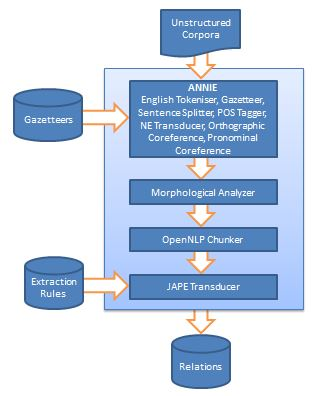
\includegraphics{archidesign1.jpg}      %-- include image file named as "sinag1.eps" 
   \caption{Architectural Design}
    \label{fig:archidesign}
\end{figure}

Each children's story text from the \textit{unstructured corpora} is opened in GATE by creating a GATE Document. Once the GATE documents are created, the next step is to create a GATE Corpus and add the documents. First, the GATE application resets the input of any previous annotations. This applies only if the input has already been annotated before passing through GATE. After cleaning, the input is parsed into tokens. The input was then  split into sentences and each token was annotated with their respective part-of-speech tags. After that, named-entities from the defined gazetteers were annotated. Then, pronouns are matched with the named-entities they are referring to in the text. 

Then, each token are processed to identify their lemmas, affixes and chunks. Lastly, the input text is ran through a transducer. This finally identify all the target relations and create the appropriate annotations for each.

The output of the GATE tool is an annotated version of the story that also contain the extracted target relations.

\subsubsection{Resolving Story-specific Named Entities}
\label{sec:gazetteer}

In this implementation, a gazetteer resource was used to identify named entities in the input texts. However, the predefined lists does not cover some of the named entities in the children's story corpora. Such include characters, locations and roles. For example, in the \textit{Winnie the Pooh} set of stories, \textit{Pooh}, \textit{Piglet} and \textit{Tigger}, among others, are not included. Thus, additional lists are needed. Aside from the named entities found in stories, gazetteers are also created for indicators, world states and emotions, among others. These were used by the transducer in its annotation patterns. A total of 20 new gazetteers were created for this study. Shown in Table \ref{tab:newgazetteersind} are the gazetteers created for indicators.

\begin{table}[H]   %t means place on top, replace with b if you want to place at the bottom
\centering
\caption{New Gazetteers (Indicators)} \vspace{0.25em}
\begin{tabular}{|p{5cm}|p{5cm}|} \hline
\textbf{File Name} & \textbf{Description} \\ \hline
isaindicator.lst			& IsA Indicators \\ \hline
partofindicator.lst			& PartOf Indicators \\ \hline
madeofindicator.lst			& MadeOf Indicators \\ \hline
oftennearindicator.lst		& OftenNear Indicators \\ \hline
capableofindicator.lst		& CapableOf Indicators \\ \hline
locationofindicator.lst		& LocationOf Indicators \\ \hline
usedforindicator.lst		& UsedFor Indicators \\ \hline
ownsindicator.lst 			& Owns Indicators \\ \hline
motivationindicator.lst		& Motivation Indicators \\ \hline
goalindicator.lst			& Goal Indicators \\ \hline
causeindicator.lst			& Cause Indicators \\ \hline
effectindicator.lst			& Effect Indicators \\ \hline
\end{tabular}
\label{tab:newgazetteersind}
\end{table}

Table \ref{tab:newgazetteersstory} shows the gazetteers created for the story characters, locations and objects. Others were added to assist in improving the extraction of target relations.

\begin{table}[H]   %t means place on top, replace with b if you want to place at the bottom
\centering
\caption{New Gazetteers (Miscellaneous)} \vspace{0.25em}
\begin{tabular}{|p{5cm}|p{5cm}|} \hline
\textbf{File Name} & \textbf{Description} \\ \hline
storyLoc.lst		& Story Locations \\ \hline
animal.lst			& Animals \\ \hline
bodypart.lst		& Body Parts \\ \hline
position.lst		& Spatial markers \\ \hline
object.lst			& Objects \\ \hline
character.lst		& Story Characters \\ \hline
emotion.lst			& Emotions \\ \hline
worldstate.lst 		& World States \\ \hline
\end{tabular}
\label{tab:newgazetteersstory}
\end{table}

\subsubsection{Recognizing Target Relations}
\label{sec:recogtarget}

In order to extract the target relations, a number of JAPE phases must be created to recognise and annotate them in the input texts. A total of 23 customized JAPE phases were created for this purpose. Shown in Table \ref{tab:newjaperel} are the new JAPE phases to recognize the target relations. 

\begin{table}[H]   %t means place on top, replace with b if you want to place at the bottom
\centering
\caption{New JAPE Phases (Target Relations)} \vspace{0.25em}
\begin{tabular}{|p{6cm}|p{5cm}|} \hline
\textbf{File Name} & \textbf{Description} \\ \hline
isARelation.jape					& IsA Phase \\ \hline
partOfRelation.jape					& PartOf Phase \\ \hline
madeOfRelation.jape					& MadeOf Phase \\ \hline
oftenNearRelation.jape				& OftenNear Phase \\ \hline
capableOfRelation.jape				& CapableOf Phase \\ \hline
locationOfRelation.jape				& LocationOf Phase \\ \hline
usedForRelation.jape				& UsedFor Phase \\ \hline
ownsRelation.jape 					& Owns Phase \\ \hline
effectOf.jape						& EffectOf Phase \\ \hline
effectOfIsState.jape				& EffectOfIsState Phase \\ \hline
eventForGoalEvent.jape				& EventForGoalEvent Phase \\ \hline
eventForGoalState.jape				& EventForGoalState Phase \\ \hline
happens.jape						& Happens Phase \\ \hline
hasRoleRelation.jape				& HasRole Phase \\ \hline
roleResponsibleForRelation.jape		& RoleResponsibleFor Phase \\ \hline
\end{tabular}
\label{tab:newjaperel}
\end{table}

Table \ref{tab:newjapemisc} shows the other JAPE phases that are prerequisites of the target relation JAPE phases. These tag the custom tags \textit{Event}, \textit{Goal}, \textit{GoalEvent}, \textit{GoalState}, \textit{Cause} and \textit{Effect}. \textit{Preprocessing1.jape} is responsible in identifying the named-entities added for the benefit of the existing corpora.

\begin{table}[H]   %t means place on top, replace with b if you want to place at the bottom
\centering
\caption{New JAPE Phases (Miscellaneous)} \vspace{0.25em}
\begin{tabular}{|p{5cm}|p{5cm}|} \hline
\textbf{File Name} & \textbf{Description} \\ \hline
cause.jape				& Identify causes \\ \hline
effect.jape				& Identify effects \\ \hline
event.jape				& Identify events \\ \hline
goal.jape				& Identify goals \\ \hline
goalEvent.jape			& Identify goal events \\ \hline
goalState.jape			& Identify goal states \\ \hline
preprocessing1.jape		& Identify named entities based on new gazetteers \\ \hline
\end{tabular}
\label{tab:newjapemisc}
\end{table}

The JAPE tool follows a sequence in performing the aforementioned phases. Shown below is the sequence in tagging the custom tags and extracting the target relations:

\begin{verse}
\itshape
preprocessing1 \\
goal \\
goalEvent\\
goalState\\
event\\
cause\\
effect\\
isARelation\\
propertyOfRelation\\
madeOfRelation\\
oftenNearRelation\\
locationOfRelation\\
capableOfRelation\\
usedForRelation\\
ownsRelation\\
hasRoleRelation\\
partOfRelation\\
roleResponsibleForRelation\\
eventForGoalEvent\\
eventForGoalState\\
effectOf\\
effectOfIsState\\
happens\\
\end{verse}

\textit{Preprocessing1.jape} is the first phase ran to identify and tag all the new named-entities found in the corpora. This is followed by the tagging of \textit{Event}, \textit{Goal}, \textit{GoalEvent}, \textit{GoalState}, \textit{Cause} and \textit{Effect}. These are prerequisites for the \textit{EventForGoalEvent}, \textit{EventForGoalState}, \textit{EffectOf},  \textit{EffectOfIsState} and \textit{Happens} phases. The rest of the phases were put in that sequence based on the order of their creation.

During each phase, the whole document is processed. This allows multiple relation types to be extracted from a single sentence.

\subsection{Post-Processing}
\label{sec:postprocessing}

After running the GATE tool to annotate the stories, all post-processing were done semi-automatically. Since the output of GATE is just the annotated version of the input corpus, the annotated stories were saved as XML from the GATE program. These XML files contain all annotations like \textit{Token} and \textit{Sentence}, among others.  The target relations were then extracted to a PBREL file. 

PBREL files are created for the purpose of this study. It contains all extracted target relations from a story. Aside from the relations and their corresponding concepts, the rules used to extract them are also included for debugging purposes. An excerpt from \textit{A wild weather day.pbrel} is shown below.

\begin{verse}
\itshape
UsedFor(snacks,eating) UsedForRelation3 \\
Owns(their,adventure) OwnsRelation3\\
Owns(Pierre,garden) OwnsRelation3\\
CapableOf(thunder,go) CapableOfRelation1\\
EffectOf(stopped blowing,stopped falling) EffectOf4\\
EffectOf(shook the clubhouse,looked out the window) EffectOf4\\
EffectOf(got really cold,turned into balls of ice) EffectOf4\\
\end{verse}

After creating PBREL files for each story, the extracted relations were then collated into a single CPBREL (Collated PBREL) file for each big group of stories (\emph{RAW} and \emph{MODIFIED}). Aside from collating, redundant relations were also removed. The final CPBREL files for the \emph{RAW} and \emph{MODIFIED} stories were used in the testing stage.







               %-- includes LaTeX source file for Chapter 4: Design and Implementation
                                  %-- your job: **EDIT THIS FILE** to indicate your design and implementation
                                  
%%%%%%%%%%%%%%%%%%%%%%%%%%%%%%%%%%%%%%%%%%%%%%%%%%%%%%%%%%%%%%%%%%%%%%%%%%%%%%%%%%%%%%%%%%%%%%%%%%%%%%
%
%   Filename    : chapter_5.tex 
%
%   Description : This file will contain your Results and Analysis.
%                 
%%%%%%%%%%%%%%%%%%%%%%%%%%%%%%%%%%%%%%%%%%%%%%%%%%%%%%%%%%%%%%%%%%%%%%%%%%%%%%%%%%%%%%%%%%%%%%%%%%%%%%

\Section{Results and Analysis}
\label{sec:resultsandanalysis}

This chapter discusses the overall quality of the extracted relations. It also describes the results and the methodology in evaluating them.

\subsection{Methodology}
\label{sec:methodology}

This section details the strategies employed in evaluating the quality and completeness of the extracted relations.

\subsubsection{Quantitative Evaluation}

A gold standard was 

\subsubsection{Story Evaluation}

In order to validate the quality of the extracted relations, they were used to generate stories in Picture Books. First, Picture Books was examined to determine which themes can be used. Then, the target relations extracted from the \textit{RAW} and \textit{MODIFIED} corpora were evaluated to see whether any of them can be easily inserted into the existing Picture Books ontology. Additional relations were manually added by the researcher for the target relations which did not have valid extractions from either corpora. Then, the Picture Books databases were manually updated with a select number of valid extractions, as well as the additional ones. 

\subsubsection*{Examining the Picture Books Themes}
\label{sec:examinethemes}

Aside from checking the valid extractions that can be used for testing, the themes of Picture Books were also examined. There are two motivations for this. First, the researcher would like to determine which among the themes can be used for testing. And secondly, he would like to map which target relation types can be tested for each theme selected.

After carefully tracing the ontology accesses and searches within the 15 different themes, five (5) were identified. Table \ref{tab:mapthemerel} shows the themes selected for testing with the mapped target relation types.

\begin{table}[H]   %t means place on top, replace with b if you want to place at the bottom
\centering
\caption{Mapping of Picture Books Themes with Target Relation Types} \vspace{0.25em}
\begin{tabular}{|p{5cm}|p{5cm}|} \hline
\textbf{Theme ID and Lesson} & \textbf{Mapped Target Relation Types} \\ \hline
THME0001: Take Bath			& usedFor \\ \hline
THME0003: Be Careful		& isA, capableOf, effectOf, propertyOf \\ \hline
THME0012: Be Honest			& isA, capableOf, effectOf, propertyOf \\ \hline
THME0005: Be Neat			& eventForGoalEvent \\ \hline
THME0015: Be Brave			& effectOfIsState \\ \hline
\end{tabular}
\label{tab:mapthemerel}
\end{table}  

After examination, only 7 target relation types were possible to be tested using the existing Picture Books themes.

\subsubsection*{Grouping Target Relation Types}
\label{sec:grouprel}

Since only 7 target relation types can be tested by branching the existing ontology accesses and searches in the existing themes (See Section \ref{sec:examinethemes}), another group was created. This includes the 9 remaining target relation types which were not present in any of Picture Books' existing themes. A summary of the grouping is shown in Table \ref{tab:relgroups}.

\begin{table}[H]   %t means place on top, replace with b if you want to place at the bottom
\centering
\caption{Target Relation Type Groups} \vspace{0.25em}
\begin{tabular}{|p{5cm}|p{5cm}|} \hline
\textbf{Group A: Used in existing themes} & \textbf{Group B: Not used in existing themes} \\ \hline
isA, capableOf, propertyOf, effectOf, effectOfIsState, usedFor, eventForGoalEvent	& locationOf, partOf, madeOf, eventForGoalState, oftenNear, happens, hasRole, roleResponsibleFor, owns \\ \hline
\end{tabular}
\label{tab:relgroups}
\end{table}

\emph{Group A Relations}

For this group, 9 new lexicon entries and 12 new concepts were added into the database. The discrepancy was due to the words already existing in the lexicon but not as concepts to be used for ontology searches. Then, forty-one (41) new ontology entries were added to branch from existing ontology searches. Shown in Figure \ref{fig:altpath} is a sample alternative path created for this study. This is for author goal AUTH0026 of theme THME0003 (Be Careful).

\begin{figure}[h]                %-- use [t] to place figure at top, [b] to place at the bottom
   \centering                    %-- use this to center the figure
   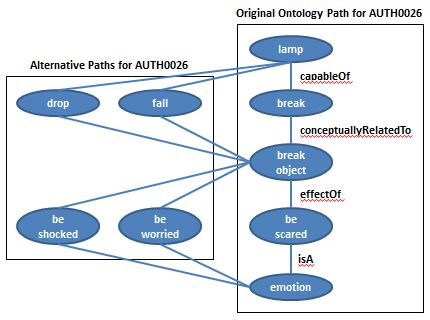
\includegraphics{altpath.jpg}      %-- include image file named as "sinag1.eps" 
   \caption{Alternative Path for AUTH0026}
    \label{fig:altpath}
\end{figure}

From the figure, there were 4 new concepts added and 8 new relations (2 \textit{IsA}, 2 \textit{ConceptuallyRelatedTo}, 2 \textit{EffectOf} and 2  \textit{CapableOf}). Though the relation \textit{ConceptuallyRelatedTo} is not really a target relation for this study, such entries were still created to maintain the path going to the last node (\textit{emotion}). 

However, as an exceptional case in this group of relations, the \textit{EffectOfIsState} relation was configured differently. Aside from the additional lexicon entries, concepts and ontology entries, 2 new author goals and 2 new story plot trackers were created. The new story plot trackers were then added as alternative Solutions to the theme THME0015 (Be Brave). This is all due to the difference in accessing the \textit{EffectOfIsState} in the author goal AUTH0056. Figure \ref{fig:altpatheffectofisstate} shows how the relation was accessed in the path. Instead of accessing the relation in the middle of the path, it was done at the end which was explicitly indicated in the definition of the author goal AUTH0056. This means there is no way to randomly select a new concept. 

\begin{figure}[h]                %-- use [t] to place figure at top, [b] to place at the bottom
   \centering                    %-- use this to center the figure
   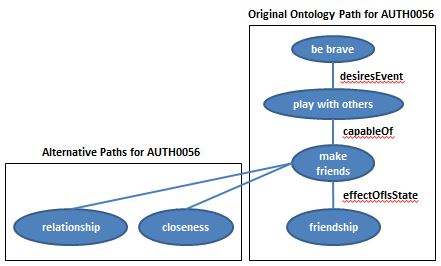
\includegraphics{altpatheffectofisstate.jpg}      %-- include image file named as "sinag1.eps" 
   \caption{Alternative Path for AUTH0056}
    \label{fig:altpatheffectofisstate}
\end{figure}

Appendix E shows all the additional entries in the Picture Books lexicon and ontology.

\emph{Group B Relations}

Because Group B relations did not exist in the current version of Picture Books' ontology, author goals were created to show the relations in the generated stories. 16 new lexicon entries and 20 new concepts were added into the database. Then, 27 new ontology entries were added. Finally, 9 new author goals were created and inserted as additional author goals of story plot tracker SPAT0004. 

For this group of relations, the theme THME0001 (Take Bath) was used. Each relation type had 2 representative sentences created and were included in the final story generated. None of the concepts and sentences were made coherent to the rest of the story. Appendix E shows all the additional entries in the Picture Books lexicon and ontology.

\subsubsection*{Selected Relations}
\label{sec:selectedrelations}

Out of all the extracted relations from the \textit{RAW} and \textit{MODIFIED} corpora, only 6 relations were used and all of them are \textit{PartOf} relations. The rest of the relations used for testing were manually created. 

Group A needed extracted relations that are related to the themes selected as they are embedded in the ontology searches and accesses. But none of the extracted relations that fall under this group were coherent to any of the themes. \textit{EffectOfIsState} was also not extracted. Thus, it was decided to just create new relations that would be coherent to the rest of the stories. 

Group B, on the other hand, did not require the extracted relation to be coherent to the theme \textit{Take Bath} because that was not the intention. But because \textit{MadeOf} and \textit{OftenNear} were not extracted at all and \textit{EventForGoalState}, \textit{Happens}, \textit{HasRole}, \textit{Owns} and \textit{RoleResponsibleFor} did not have valid extractions, manual entries were also created.

\subsection{Extraction Analysis}
\label{sec:extractionanalysis}

\subsubsection{Uniqueness and Redundancies}

In this evaluation, the number of unique extractions were analyzed to determine whether the modifications created more relations valid for extraction. Also, duplicate or redundant extractions are also analyzed to see whether they were reduced after modification.

There was a total of 13,871 unique relations extracted from the \textit{RAW} and \textit{MODIFIED} corpora. Tables \ref{tab:modifiedtotal} and \ref{tab:rawtotal} show the breakdown of numbers for each group of stories in each corpora.

\begin{table}[H]   %t means place on top, replace with b if you want to place at the bottom
\centering
\caption{Raw Corpus: Number of Unique and Redundant Relations Extracted} \vspace{0.25em}
\begin{tabular}{|p{4cm}|p{3cm}|p{3cm}|} \hline
\textbf{Story Group} & \textbf{Unique} & \textbf{Redundant} \\ \hline
Jumpstart & 644 & 194 \\ \hline
Winnie the Pooh & 394 & 94 \\ \hline
Topsy Tim & 684 & 215 \\ \hline
Little Life Lessons & 4977 & 2017 \\ \hline
\textbf{TOTAL} & \textbf{6699} & \textbf{2520} \\ \hline
\end{tabular}
\label{tab:rawtotal}
\end{table}

\begin{table}[H]   %t means place on top, replace with b if you want to place at the bottom
\centering
\caption{Modified Corpus: Number of Unique and Redundant Relations Extracted} \vspace{0.25em}
\begin{tabular}{|p{4cm}|p{3cm}|p{3cm}|} \hline
\textbf{Story Group} & \textbf{Unique} & \textbf{Redundant} \\ \hline
Jumpstart & 729 & 206 \\ \hline
Winnie the Pooh & 436 & 137 \\ \hline
Topsy Tim & 747 & 341 \\ \hline
Little Life Lessons & 5260 & 2621 \\ \hline
\textbf{TOTAL} & \textbf{7172} & \textbf{3305} \\ \hline
\end{tabular}
\label{tab:modifiedtotal}
\end{table}

From these numbers, it is evident that the \textit{Modified} corpus had 473 more relations extracted than the \textit{Raw} corpus. This suggests that the modifications done introduced new concepts, thus allowing the application to extract more unique relations. These modifications may have also introduced more redundant relations as the number increased by 785. This was even more than the increase in unique relations. Here are sample passages from \textit{CJ and the Mysterious Map}:

\begin{verse}
\itshape
``And how do you suggest we get up there?" asked Edison.\\
``What are you doing?" asked Edison.\\
\end{verse}

These are non-adjacent sentences from the story. After running this in the extraction tool, they yielded zero extractions. Then they were modified to this:

\begin{verse}
\itshape
Edison asked CJ some suggestions.\\
Edison asked what CJ is doing.\\
\end{verse}

Now, each sentence was able to produce 2 new \textit{CapableOf} extractions. However, both of them are \textit{CapableOf(Edison,ask)}. And after examining the modified story, there were more sentences of this structure that yielded the same relation. 

In terms of relations, Table \ref{tab:reltotal} shows the breakdown of extracted relations per corpora. The delta after modification is also shown. 

\begin{table}[H]   %t means place on top, replace with b if you want to place at the bottom
\centering
\caption{Number of Relations Extracted per Corpus} \vspace{0.25em}
\begin{tabular}{|p{4.5cm}|p{2cm}|p{2cm}|p{2cm}|} \hline
\textbf{Relations} & \textbf{Raw} & \textbf{Modified} & \textbf{Delta} \\ \hline
IsA & 191 & 228 & 37 \\ \hline
PropertyOf & 2700 & 2857 & 157 \\ \hline
PartOf  & 71 & 84 & 13 \\ \hline
MadeOf & 0 & 0 & 0 \\ \hline
EventForGoalEvent & 481 & 580 & 99 \\ \hline
EventForGoalState & 31 & 37 & 6 \\ \hline
EffectOf & 1258 & 1196 & -62 \\ \hline
EffectOfIsState & 0 & 0 & 0 \\ \hline
CapableOf & 980 & 1193 & 213 \\ \hline
OftenNear & 0 & 0 & 0 \\ \hline
LocationOf & 136 & 137 & 1 \\ \hline
UsedFor & 228 & 232 & 4 \\ \hline
Happens & 38 & 34 & -4 \\ \hline
HasRole & 11 & 14 & 3 \\ \hline
RoleResponsibleFor & 11 & 13 & 2 \\ \hline
Owns & 562 & 565 & 3 \\ \hline
\end{tabular}
\label{tab:reltotal}
\end{table}

In a relational level, almost all relations experienced an increase in the number of extractions except for \textit{EffectOf} and \textit{Happens}. Again, although the delta is not significant in number, it suggests that the modifications avoided the extraction of possible relations. Here is an  extracted relation from the \textit{Raw} corpus that is not included as an extracted relation in the \textit{Modified} corpus:

\begin{verse}
\itshape
EffectOf(said,not forgive and forget)
\end{verse}

It was extracted from this passage from \textit{Forgive and Forget} of the \textit{Winnie the Pooh} story group:

\begin{verse}
\itshape
``Rabbit, I think Tigger is very sorry," Pooh said. ``Will you not forgive and forget?"
\end{verse}

This specific sentence was modified to this:

\begin{verse}
\itshape
Pooh thinks Tigger is very sorry. Pooh asks Rabbit if he can forgive and forget.
\end{verse}

In this example, the verb \textit{said} was removed after modification, thus avoiding the possibility of another relation being extracted. It seems that modifications, such as this, improved the result for the \textit{Modified} corpus because the relation is not really a valid and logical extraction. However, the possibility that valid extractions may also be omitted in the process cannot be discounted.

\subsubsection{Zero Extraction}

From the same table, it is important to note that the \textit{EffectOfIsState}, \textit{MadeOf} and \textit{OftenNear} relations had 0 extractions from either corpora. This was caused by their high dependence on indicators, incorrect part-of-speech tags and limitation on the number of sentences it can extract from. 

\subsubsection{Quality}

In terms of extraction quality, there are some relations which may have been incorrectly extracted or which may not be extracted at all because of incorrect tags. For instance, this relation was extracted from the \textit{Jumpstart} story group:

\begin{verse}
\itshape
EffectOf(went on full speed,shocked)
\end{verse}

The extraction seems valid from first glance, but looking at its original passage may suggest otherwise. Shown below is the modified passage from \textit{Just in time}. Instead of \textit{EffectOf}, a better extraction could have been \textit{EffectOfIsState} since \textit{being shocked} is an implied state. 

\begin{verse}
\itshape
Frankie went on full speed.\\
Hopsalot was shocked.
\end{verse}

Other incorrect extractions were due to a different part-of-speech information tagged to the concept and the lack of additional semantic information.

Lastly, it is important to note that for event relations like \textit{EffectOf} and \textit{EventForGoalEvent}, the extracted relations seem to be longer and more specific because the extractor uses whole phrases as concepts. This may be different from the concepts of Picture Books that are more generalized. Here are some example extractions:

\begin{verse}
\itshape
EffectOf(looked at the map,checked the wind)\\
EffectOf(pours something into the volcano,stopped him)\\
EventForGoalEvent(called everyone,go to the ship)
\end{verse}

For a more detailed look in the extraction results, kindly refer to Appendix D.

\subsection{Story Analysis}
\label{sec:storyanalysis}

Overall, the new relations were used accordingly. They were randomly selected and used interchangeably with the original relations. But the sentences generated were fairly acceptable. There are cases wherein the sentence is grammatically incorrect. For example, here is an original story generated for the \textit{Be Careful} theme:

\begin{alltt}
\textbf{Edward the elephant learns to be careful.}

[1]  The morning was sunny.
[2]  Edward the elephant was in the dining room.
[3]  He played near breakable glass of water.
[4]  Daddy Sam told Edward to be careful.
[5]  Edward continued to play glass of water near.
\underline{\emph{\textbf{[6]  He broke it.}}}
\underline{\emph{\textbf{[7]  Edward was scared.}}}
[8]  He hid away from Daddy Sam.
\underline{\emph{\textbf{[9]  Daddy Sam saw that glass of water was broken.}}}
[10] Daddy Sam called Edward.
[11] Daddy Sam told Edward that he should have obeyed.
[12] He felt sorry.
[13] Daddy Sam cleaned up glass of water.
[14] Edward helped Daddy Sam to clean up.
[15] Daddy Sam reminded Edward to be careful.
[16] Being careful is important.
[17] From that day onwards, Edward always was careful.
\end{alltt}

This used the original relations of Picture Books. The highlighted lines show the sentences where the changes should happen. Shown below is another story using the same characters and objects as the story above. This time, the highlighted sentences are using different concepts based on the new additions to the lexicon and ontology.

\begin{alltt}
\textbf{Edward the elephant learns to be careful.}

[1]  The afternoon was sunny.
[2]  Edward the elephant was in the dining room.
[3]  He played near breakable glass of water.
[4]  Mommy Edna told Edward to be careful.
[5]  Edward continued to play glass of water near.
\underline{\emph{\textbf{[6]  Edward fell it.}}}
\underline{\emph{\textbf{[7]  Edward was worried.}}}
[8]  He hid away from Mommy Edna.
\underline{\emph{\textbf{[9]  Mommy Edna saw that glass of water was cracked.}}}
[10] Mommy Edna called Edward.
[11] Mommy Edna told Edward that he should have obeyed.
[12] Edward felt sorry.
[13] Mommy Edna cleaned up glass of water.
[14] Edward helped Mommy Edna to clean up.
[15] She reminded Edward to be careful.
[16] Being careful is important.
[17] From that day onwards, Edward always was careful.
\end{alltt}

In line 6, instead of the usual action \textit{broke}, the story now uses \textit{fell}. However, the new sentence should have been ``It fell" or ``The glass of water fell." Since the relation used here is \textit{CapableOf(lamp,fall)}, it also logical to note that the \textit{lamp} can be the agent of the action instead of always being the character. 

Another new story worth pointing out is this:

\begin{alltt}
\textbf{Edward the elephant learns to be honest.}

[1]  The morning was warm.
[2]  Edward the elephant was in the dining room.
[3]  He played near breakable glass of water.
\underline{\emph{\textbf{[4]  Edward fell glass of water.}}}
[5]  He was worried.
[6]  Mommy Edna saw that glass of water was smashed.
[7]  Edward told Mommy Edna that Porky the pig broke glass of water.
[8]  He was sad.
[9]  Porky cried.
[10] Edward felt guilty.
\underline{\emph{\textbf{[11] Edward told Mommy Edna that he dropped glass of water.}}}
[12] Mommy Edna told Edward that he should have been honest.
[13] He apologized to Mommy Edna.
[14] Edward apologized to Porky.
[15] Mommy Edna told Edward to be honest.
[16] Mommy Edna told Edward that being honest is good.
[17] From that day onwards, Edward always was honest.
\end{alltt}

In this story, highlighted are the sentences using the \textit{CapableOf} relations with \textit{lamp} as the parent concept, \textit{CapableOf(lamp,fall)} and \textit{CapableOf(lamp,drop)}. Though it is valid to use both, having them in just one story creates inconsistencies. In line 4, it was already mentioned that the glass of water fell. And since the word \textit{fell} was used, there is an implication of an accident which creates a different dimension to the story. Now in line 11, though Edward is already admitting his fault, he suddenly said \textit{dropped} instead of the initial \textit{fell}. This might create confusion as dropping something makes the act intentional whereas when it fell, Edward may or may not have caused the action. When the act \textit{fell} was used in line 4, it expected that the same act is confessed in line 11.

Lastly, there are a number of instances where incorrect relations are picked up by Picture Books in doing ontology accesses and searches. As a result, incorrect sentences are generated. For example, in the story \textit{Roy the chicken learns to take bath.} shown below, lines 9 and 10 are produced using the same relation, \textit{OftenNear}. They also have the same parent concept which is \textit{school}. Line 9 has a correct child concept but Line 10 does not. Instead of either \textit{clinic}, \textit{mall} or \textit{market}, it used \textit{generic}. After examining the ontology, \textit{generic} is the child concept when the relation is \textit{PropertyOf}. This shouldn't be the case. 

The reason why this happens is because Picture Books searches its ontology not by the name of the relation but by its category. In the ontology, both \textit{OftenNear} and \textit{PropertyOf} are under the category \textit{spatial}. This causes Picture Books to not only randomize among \textit{OftenNear} relations but also including the \textit{PropertyOf} relation.

\begin{alltt}
[1]  Toys were the bedroom.
[2]  Playing is the playground.
[3]  An oak had trunk.
[4]  A person had a toe.
[5]  A book had paper.
[6]  It had ink.
[7]  Playing is dirty.
[8]  It was healthy.
\underline{\emph{\textbf{[9]  The school was the market.}}}
\underline{\emph{\textbf{[10] It was generic.}}}
[11] Eating dinner is the evening.
[12] Going to the school is the morning.
[13] A fireman was rescuing.
[14] A librarian was organizing.
[15] Daddy Sam had a ball.
[16] He had the tricycle.
[17] From then on, Roy always took the bath.
\end{alltt}

Another example is with the same story but lines 11 and 12 are changed to the following:

\begin{alltt}
[11] Eating dinner is the evening.
\underline{[12] Going to the school is \emph{\textbf{saying goodbye}}.}
\end{alltt}

These two sentences are using the \textit{Happens} relation. But in line 12, the relation \textit{FirstSubeventOf} was used because they are both \textit{event} relations. This happens for ontology accesses that only have 1 argument.

Kindly refer to Appendix F for all the stories generated in this phase.









               %-- includes LaTeX source file for Chapter 5: Results and Analysis
                                  %-- your job: **EDIT THIS FILE** to indicate your results and analysis
                                  
%%%%%%%%%%%%%%%%%%%%%%%%%%%%%%%%%%%%%%%%%%%%%%%%%%%%%%%%%%%%%%%%%%%%%%%%%%%%%%%%%%%%%%%%%%%%%%%%%%%%%%
%
%   Filename    : chapter_6.tex 
%
%   Description : This file will contain your Conclusion and Recommendations.
%                 
%%%%%%%%%%%%%%%%%%%%%%%%%%%%%%%%%%%%%%%%%%%%%%%%%%%%%%%%%%%%%%%%%%%%%%%%%%%%%%%%%%%%%%%%%%%%%%%%%%%%%%

\Section{Conclusion and Recommendations}
\label{sec:conclusionandreco}

This chapter discusses the conclusion of this research and provides recommendations and suggestions for future researches.

\subsection{Conclusion}
\label{sec:conclusion}

Based on the results obtained through the evaluation of the extractor, it was proven possible to extract new semantic relations from children's stories and feed them into Picture Books' ontology. However, the extractor was found to be inaccurate in doing so. Overall, it only got 0.36 as its precision, recall and F-measure scores for 3 MODIFIED stories. It even got lower scores for the RAW versions. It got 0.34, 0.32 and 0.33 for its precision, recall and F-measure, respectively. Therefore, the automatically extracted relations were mostly incorrect and the extractor was not able to extract all expected relations in a given text.

New relations were used accordingly and interchangeably, and new sentences were inserted. However, due to the limited themes currently present in Picture Books, not all extracted relations was used. There were also cases wherein all extracted relations won't be valid for Picture Books' use because the story where they came from are completely different from the existing themes. Another issue was Picture Books' way of accessing its ontology. Instead of using the relation names as reference, the relation category is used. Since each category has more than 1 relation associated, incorrect searches may still arise. Thus rendering the attempt to improve Picture Books' conceptual knowledge less remarkable. Lastly, it is not enough to just add new concepts and relations in the current ontology. Additional steps must be taken depending on how the ontology path you are trying to branch is accessed.

As for the extracted relations, their quality was greatly affected by the following:

\subsubsection{Stories}
\label{sec:stories}

Each story in the corpora has different characteristics. Some are lengthy while some are short. Some use a lot of complex sentence structures while others kept it simple. It all depends on the age group of the audience they are trying to reach. After evaluation, it is conclusive that as the sentence structures become more complex and the length of the story increases, the extractions get less accurate. It exposes a limitation on the templates used as they can only successfully handle simpler sentences and simpler manifestations of a relation in a text.

\subsubsection{Part-of-speech Tags}
\label{sec:pos}

The quality and accuracy of the part-of-speech tags supplied by GATE greatly affected the relations extracted. Because most of the extraction rules/templates mainly use part-of-speech tags in their annotation patterns, a slight mistake may cause the relation to have incorrect concepts or to have it not extracted at all. Here is a sample sentence to illustrate this scenario:

\begin{verse}
\itshape
Tigger takes a bath because he wants to be clean.
\end{verse}

One relation that can be extracted from this would be \textit{EventForGoalState(takes a bath,be clean)}. However, after numerous attempts in the application, that relation will not be extracted because \textit{clean} is tagged as a verb. The researcher's rule for \textit{EventForGoalState} requires the child concept to be an adjective for it to be called a desired state.

\subsubsection{Extraction rules}
\label{sec:templates}

Because the current set of extraction rules are generalized based on ConceptNet sentence patterns and the sentences present in the current corpora, there is a perceived limit in the capabilities of the extractor. And in the attempt to cover all sentence patterns with the least number of rules, exceptional cases may not be covered. Also, these rules cannot handle implied and inferred relations. If there are any implied or inferred ones in the text, the rules won't recognize them unless they were explicitly indicated after modification. Additionally, these rules do not have enough semantic information for most words. When a different sense of a word is used in a sentence, there is no way for the extractor to recognise it. It will rely solely on the part-of-speech and named-entity tags to extract a relation. This deficiency in semantic information also causes an incorrect relation to be tagged to a concept pair. For example, \textit{PartOf} relations can be incorrectly tagged as an \textit{Owns} relation because of the similarity in templates used.  Lastly, the templates were also limited to 1 or 2 sentences only. Most of the relations encountered in the gold standard were identified from sentence more than 2 sentences apart. 

\subsubsection{Indicators}
\label{sec:indicators}

The prevalent use of indicators in most of the extraction templates posed a limitation on the number and quality of extractions done. First, in most cases, indicators are not always used because of their formality. This also assumes that the concepts constituting a relation is within a sentence. If not, it is assumed that the second concept is in the next sentence, the subject pronoun referring to the first concept, and the whole thing signalled by an indicator.

Secondly, most relations identified in the gold standard were inferred or implied. Taking a look into the \textit{HasRole} relation again, the only instance did not have both concepts present in the story. In the relation \textit{HasRole(Miss Hen,teacher)}, the word \textit{teacher} was not found in the text. It was inferred as a role through the actions done by the character. Lastly, existing indicators are not enough. There's still a number of indicators not included in this study. This caused the only expected \textit{OftenNear} relation in \textit{Everybody Cries} to not be extracted. It was signalled by the word \textit{along} which is not part of the \textit{OftenNear} indicators.

\subsection{Recommendations}
\label{sec:reco}

Overall, the relation extractor was able to produce good enough relations to be used by any story generation system. The following are recommendations for future improvement:

\begin{itemize}
\item Improve the extraction rules. Incorporate as many patterns as possible. If allowable, run a big corpora through a machine learning tool that will learn all possible sentence patterns for each relation type.
\item Allow inferencing between relations as they are extracted. This will improve the compactness of the ontology.
\item Focus more on extracting event relations since they are not usually explicitly indicated in a span of text. This also constitutes the bulk of a story. Building an accurate cause-effect chain of events would be very beneficial for most creative text generation systems.
\item Look for a language resource that can supply accurate semantic information.
\item Since a gold standard was already utilized in evaluating this research, it would be beneficial to look for experts that can create different sets of gold standards for the different relations to improve the evaluation of the results. These sets could then be combined to form a comprehensive gold standard. Aside from this, have experts that can consistently evaluate the generated story after adding new relations. 
\end{itemize}

And because part of the evaluation involved the use of Picture Books in generating stories, some issues and limitations were encountered. The following are recommendations for Picture Books' future improvement:

\begin{itemize}
\item Since it is now possible to branch out in ontology searches, it would be advisable to keep track of previously chosen concepts that is expected to be used throughout the story. This will avoid conflicting details and make the output stories more coherent.
\item To be able to use all extracted relations, devise a way to automatically add new themes in Picture Books based on the themes found in the corpora. 
\item Instead of searching the ontology by category, use the relation names for more specific and accurate ontology access results.
\item Integrate VerbNet to make the character goals dynamic in creating sentences. This will provide information on what arguments are needed in a sentence for a certain verb.
\end{itemize}









               %-- includes LaTeX source file for Chapter 6: Conclusion and Recommendations
                                  %-- your job: **EDIT THIS FILE** to indicate your rconclusion and recommendations
                                  
\appendix                         %-- used to specify appendices
%%%%%%%%%%%%%%%%%%%%%%%%%%%%%%%%%%%%%%%%%%%%%%%%%%%%%%%%%%%%%%%%%%%%%%%%%%%%%%%%%%%%%%%%%%%%%%%%%%%%%%
%
%   Filename    : appendix_resourceperson.tex
%
%   Description : This file will contain information about your Resource Persons
%                 
%%%%%%%%%%%%%%%%%%%%%%%%%%%%%%%%%%%%%%%%%%%%%%%%%%%%%%%%%%%%%%%%%%%%%%%%%%%%%%%%%%%%%%%%%%%%%%%%%%%%%%
\Section{Resource Persons}
\label{sec:appendixresourceperson}

%
%  Indicate your resource persons here:
%
%	<full name and title, e.g., Dr. Juan de la Cruz>
%	<profession, e.g., faculty>
%	<department, e.g., College of Computer Studies>
%	<name of institution, e.g., De La Salle University>
%	<e-mail address>
%
%

%
%  the following shows 3 examples, replace entries with your own
%
\newcommand{\resperson}[4]{\textbf{#1} \\ #2 \\ #3 \\ \url{#4}\vspace{0.5em}\\}

\resperson{Ms. Ethel Ong}{Adviser}{College of Computer Studies\\De La Salle University-Manila}{ethel.ong@delasalle.ph}

              %-- includes LaTeX source file for Appendix A
                                  %-- your job: **CREATE/EDIT** your own source file for the appendices
%%%%%%%%%%%%%%%%%%%%%%%%%%%%%%%%%%%%%%%%%%%%%%%%%%%%%%%%%%%%%%%%%%%%%%%%%%%%%%%%%%%%%%%%%%%%%%%%%%%%%%
%
%   Filename    : appendix_personalvitae.tex
%
%   Description : This file will contain information about your Personal Vitae
%                 
%%%%%%%%%%%%%%%%%%%%%%%%%%%%%%%%%%%%%%%%%%%%%%%%%%%%%%%%%%%%%%%%%%%%%%%%%%%%%%%%%%%%%%%%%%%%%%%%%%%%%%
\Section{Personal Vitae}
\label{sec:appendixpersonalvitae}

%
%  Indicate your resource persons here:
%
%	<full name and title, e.g., Dr. Juan de la Cruz>
%	<profession, e.g., faculty>
%	<department, e.g., College of Computer Studies>
%	<name of institution, e.g., De La Salle University>
%	<e-mail address>
%
%

%
%  the following shows 3 examples, replace entries with your own
%
\newcommand{\cv}[4]{\textbf{#1} \\ #2 \\ #3 \\ \url{#4}\vspace{0.5em}\\}

\cv{Mr. Briane Paul V. Samson}{11 Gen. Arellano St., West Rembo, Makati City}{0917-8319462}{briane.samson@yahoo.com}


%%%%%%%%%%%%%%%%%%%%%%%%%%%%%%%%%%%%%%%%%%%%%%%%%%%%%%%%%%%%%%%%%%%%%%%%%%%%%%%%%%%%%%%%%%%%%%%%%%%%%%
%
%   Filename    : appendix_stories.tex
%
%   Description : This file will contain information about your Stories
%                 
%%%%%%%%%%%%%%%%%%%%%%%%%%%%%%%%%%%%%%%%%%%%%%%%%%%%%%%%%%%%%%%%%%%%%%%%%%%%%%%%%%%%%%%%%%%%%%%%%%%%%%
\Section{Children's Stories}
\label{sec:appendixstories}

%
%  Indicate your resource persons here:
%
%	<full name and title, e.g., Dr. Juan de la Cruz>
%	<profession, e.g., faculty>
%	<department, e.g., College of Computer Studies>
%	<name of institution, e.g., De La Salle University>
%	<e-mail address>
%
%

%
%  the following shows 3 examples, replace entries with your own
%

In this study, there were four main story groups used in the corpora. Their author and publication details are listed below.

\noindent
\textbf{Jumpstart}
~\\
Author: Judith Bauer Stamper\\
Publisher: Scholastic\\

\noindent
\textbf{Winnie the Pooh}
~\\
Author: A. A. Milne\\
Publisher: Methuen \& Co. Ltd. (London)\\

\noindent
\textbf{Topsy Tim}
~\\
Author: Jean Adamson \& Gareth Adamson\\
Publisher: Ladybird\\

\noindent
\textbf{Little Life Lessons}
~\\
Author: Sarah Toast, Brian Conway \& Lance Raichert\\
Publisher: Publications Unlimited\\

\noindent
Table \ref{tab:stories} shows the different stories used in the corpus. 

\begin{table}[H]   %t means place on top, replace with b if you want to place at the bottom
\centering
\caption{Children's Stories} \vspace{0.25em}
\begin{tabular}{|p{2cm}|p{5cm}|p{4cm}|} \hline
\textbf{Story Code} & \textbf{Title} & \textbf{Story Group} \\ \hline
S1 & A wild weather day & Jumpstart \\ \hline
S2 & CJ and the mysterious map & Jumpstart \\ \hline
S3 & Eleanor's enormous ears & Jumpstart \\ \hline
S4 & Hopsalot's garden & Jumpstart \\ \hline
S5 & Just in time & Jumpstart \\ \hline
S6 & Lost and found in Jumpstart town & Jumpstart \\ \hline
S7 & Rain,  rain,  go away & Jumpstart \\ \hline
S8 & Everyone is special & Winnie the Pooh \\ \hline
S9 & Forgive and Forget & Winnie the Pooh \\ \hline
S10 & Go to the park & Topsy Tim \\ \hline
S11 & Have new bikes & Topsy Tim \\ \hline
S12 & In the gym & Topsy Tim \\ \hline
S13 & Learn to swim & Topsy Tim \\ \hline
S14 & Start school & Topsy Tim \\ \hline
S15 & Everybody Cries & Little Life Lessons \\ \hline
S16 & Friends Share & Little Life Lessons \\ \hline
S17 & Game Day & Little Life Lessons \\ \hline
S18 & Good Manners & Little Life Lessons \\ \hline
S19 & Helping Hands & Little Life Lessons \\ \hline
S20 & Helping Out & Little Life Lessons \\ \hline
S21 & Imagination & Little Life Lessons \\ \hline
S22 & Learning Something New & Little Life Lessons \\ \hline
S23 & Litterbug Bear & Little Life Lessons \\ \hline
S24 & Pup Tent Pals & Little Life Lessons \\ \hline
S25 & Silly Stunts & Little Life Lessons \\ \hline
S26 & The Broken Flowerpot & Little Life Lessons \\ \hline
S27 & The Lost Shoes & Little Life Lessons \\ \hline
S28 & The New Kid & Little Life Lessons \\ \hline
S29 & The Secret Fort & Little Life Lessons \\ \hline
S30 & Treasure Hunt & Little Life Lessons \\ \hline
\end{tabular}
\label{tab:stories}
\end{table}


%%%%%%%%%%%%%%%%%%%%%%%%%%%%%%%%%%%%%%%%%%%%%%%%%%%%%%%%%%%%%%%%%%%%%%%%%%%%%%%%%%%%%%%%%%%%%%%%%%%%%%
%
%   Filename    : appendix_results.tex
%
%   Description : This file will contain information about your Results
%                 
%%%%%%%%%%%%%%%%%%%%%%%%%%%%%%%%%%%%%%%%%%%%%%%%%%%%%%%%%%%%%%%%%%%%%%%%%%%%%%%%%%%%%%%%%%%%%%%%%%%%%%
\Section{Detailed Extraction Results}
\label{sec:appendixresults}

The following tables show the detailed results of the relation extraction. 

\begin{table}[H]   %t means place on top, replace with b if you want to place at the bottom
\centering
\caption{Detailed Overall Result} \vspace{0.25em}
\begin{tabular}{|l|l|l|l|l|} \hline
 & \multicolumn{2}{ |c| }{\textbf{Raw}} & \multicolumn{2}{ |c| }{\textbf{Modified}} \\ \hline
\textbf{Story Codes} & \textbf{Unique} & \textbf{Redundant} & \textbf{Unique} & \textbf{Redundant} \\ \hline
S1 & 92 & 10 & 111 & 35 \\ \hline
S2 & 267 & 61 & 218 & 36 \\ \hline
S3 & 51 & 14 & 48 & 9 \\ \hline
S4 & 75 & 18 & 68 & 16 \\ \hline
S5 & 117 & 52 & 88 & 34 \\ \hline
S6 & 58 & 23 & 54 & 41 \\ \hline
S7 & 69 & 28 & 57 & 23 \\ \hline
S8 & 232 & 66 & 213 & 50 \\ \hline
S9 & 204 & 71 & 181 & 44 \\ \hline
S10 & 142 & 58 & 125 & 38 \\ \hline
S11 & 143 & 54 & 113 & 30 \\ \hline
S12 & 200 & 93 & 191 & 56 \\ \hline
S13 & 124 & 58 & 118 & 43 \\ \hline
S14 & 138 & 78 & 137 & 48 \\ \hline
S15 & 404 & 120 & 384 & 95 \\ \hline
S16 & 305 & 98 & 258 & 65 \\ \hline
S17 & 329 & 102 & 317 & 77 \\ \hline
S18 & 381 & 162 & 356 & 101 \\ \hline
S19 & 285 & 195 & 257 & 141 \\ \hline
S20 & 350 & 154 & 399 & 182 \\ \hline
S21 & 324 & 124 & 297 & 93 \\ \hline
S22 & 335 & 268 & 313 & 190 \\ \hline
S23 & 291 & 120 & 304 & 106 \\ \hline
S24 & 326 & 149 & 320 & 126 \\ \hline
S25 & 301 & 186 & 274 & 120 \\ \hline
S26 & 299 & 132 & 278 & 122 \\ \hline
S27 & 314 & 255 & 282 & 146 \\ \hline
S28 & 298 & 221 & 261 & 174 \\ \hline
S29 & 405 & 213 & 386 & 181 \\ \hline
S30 & 313 & 122 & 291 & 98 \\ \hline
TOTAL & 7172 & 3305 & 6699 & 2520 \\ \hline
\end{tabular}
\label{tab:all}
\end{table}

\begin{table}[H]   %t means place on top, replace with b if you want to place at the bottom
\centering
\caption{Raw Corpus: Detailed Overall Result per Relation (Part 1)} \vspace{0.25em}
\begin{tabular}{|p{1.5cm}|p{.75cm}|p{1.5cm}|p{1cm}|p{1.25cm}|p{1.25cm}|p{1.5cm}|p{1.5cm}|} \hline
\textbf{Story Code} & \textbf{IsA} & \textbf{Proper-tyOf} & \textbf{Part-Of}  & \textbf{Made-Of} & \textbf{Capa-bleOf} & \textbf{Often-Near} & \textbf{Loca-tionOf} \\ \hline
S1 & 1 & 36 & 1 & 0 & 31 & 0 & 3 \\ \hline
S2 & 6 & 86 & 2 & 0 & 43 & 0 & 5 \\ \hline
S3 & 4 & 13 & 3 & 0 & 12 & 0 & 0 \\ \hline
S4 & 2 & 31 & 0 & 0 & 11 & 0 & 0 \\ \hline
S5 & 3 & 24 & 1 & 0 & 26 & 0 & 2 \\ \hline
S6 & 2 & 21 & 2 & 0 & 8 & 0 & 4 \\ \hline
S7 & 4 & 17 & 1 & 0 & 14 & 0 & 2 \\ \hline
S8 & 5 & 71 & 0 & 0 & 44 & 0 & 4 \\ \hline
S9 & 2 & 71 & 2 & 0 & 35 & 0 & 2 \\ \hline
S10 & 3 & 65 & 1 & 0 & 12 & 0 & 4 \\ \hline
S11 & 1 & 42 & 0 & 0 & 21 & 0 & 0 \\ \hline
S12 & 4 & 60 & 3 & 0 & 49 & 0 & 6 \\ \hline
S13 & 3 & 54 & 3 & 0 & 18 & 0 & 2 \\ \hline
S14 & 2 & 82 & 0 & 0 & 15 & 0 & 1 \\ \hline
S15 & 13 & 128 & 9 & 0 & 76 & 0 & 7 \\ \hline
S16 & 11 & 81 & 1 & 0 & 40 & 0 & 1 \\ \hline
S17 & 3 & 133 & 2 & 0 & 49 & 0 & 4 \\ \hline
S18 & 13 & 151 & 4 & 0 & 47 & 0 & 2 \\ \hline
S19 & 3 & 86 & 1 & 0 & 27 & 0 & 0 \\ \hline
S20 & 13 & 163 & 9 & 0 & 62 & 0 & 1 \\ \hline
S21 & 11 & 109 & 3 & 0 & 35 & 0 & 10 \\ \hline
S22 & 9 & 142 & 0 & 0 & 30 & 0 & 9 \\ \hline
S23 & 6 & 109 & 0 & 0 & 50 & 0 & 6 \\ \hline
S24 & 7 & 159 & 0 & 0 & 29 & 0 & 9 \\ \hline
S25 & 8 & 110 & 3 & 0 & 36 & 0 & 6 \\ \hline
S26 & 16 & 100 & 3 & 0 & 35 & 0 & 6 \\ \hline
S27 & 6 & 100 & 2 & 0 & 36 & 0 & 8 \\ \hline
S28 & 5 & 105 & 5 & 0 & 32 & 0 & 7 \\ \hline
S29 & 16 & 197 & 6 & 0 & 35 & 0 & 16 \\ \hline
S30 & 9 & 154 & 4 & 0 & 22 & 0 & 9 \\ \hline
TOTAL & 191 & 2700 & 71 & 0 & 980 & 0 & 136 \\ \hline
\end{tabular}
\label{tab:raw1}
\end{table}

\begin{table}[H]   %t means place on top, replace with b if you want to place at the bottom
\centering
\caption{Raw Corpus: Detailed Overall Result per Relation (Part 2)} \vspace{0.25em}
\begin{tabular}{|l|p{2cm}|p{2cm}|l|p{2cm}|} \hline
\textbf{Story Code} & \textbf{EventFor-GoalEvent} & \textbf{EventFor-GoalState} & \textbf{EffectOf} & \textbf{EffectOf-IsState} \\ \hline
S1 & 3 & 0 & 26 & 0 \\ \hline
S2 & 12 & 0 & 36 & 0 \\ \hline
S3 & 1 & 0 & 9 & 0 \\ \hline
S4 & 1 & 0 & 9 & 0 \\ \hline
S5 & 3 & 0 & 17 & 0 \\ \hline
S6 & 1 & 0 & 7 & 0 \\ \hline
S7 & 1 & 0 & 15 & 0 \\ \hline
S8 & 14 & 3 & 44 & 0 \\ \hline
S9 & 15 & 1 & 35 & 0 \\ \hline
S10 & 5 & 0 & 18 & 0 \\ \hline
S11 & 8 & 0 & 19 & 0 \\ \hline
S12 & 11 & 0 & 28 & 0 \\ \hline
S13 & 8 & 1 & 17 & 0 \\ \hline
S14 & 9 & 0 & 13 & 0 \\ \hline
S15 & 23 & 3 & 64 & 0 \\ \hline
S16 & 20 & 1 & 68 & 0 \\ \hline
S17 & 26 & 0 & 66 & 0 \\ \hline
S18 & 27 & 4 & 55 & 0 \\ \hline
S19 & 33 & 2 & 56 & 0 \\ \hline
S20 & 36 & 0 & 72 & 0 \\ \hline
S21 & 26 & 5 & 61 & 0 \\ \hline
S22 & 32 & 1 & 59 & 0 \\ \hline
S23 & 16 & 5 & 74 & 0 \\ \hline
S24 & 16 & 2 & 57 & 0 \\ \hline
S25 & 27 & 0 & 45 & 0 \\ \hline
S26 & 20 & 0 & 66 & 0 \\ \hline
S27 & 23 & 1 & 62 & 0 \\ \hline
S28 & 29 & 1 & 56 & 0 \\ \hline
S29 & 17 & 0 & 49 & 0 \\ \hline
S30 & 18 & 1 & 55 & 0 \\ \hline
TOTAL & 481 & 31 & 1258 & 0 \\ \hline
\end{tabular}
\label{tab:raw2}
\end{table}

\begin{table}[H]   %t means place on top, replace with b if you want to place at the bottom
\centering
\caption{Raw Corpus: Detailed Overall Result per Relation (Part 3)} \vspace{0.25em}
\begin{tabular}{|l|l|l|l|l|l|} \hline
\textbf{Story Code} & \textbf{UsedFor} & \textbf{Happens} & \textbf{HasRole} & \textbf{RoleResponsibleFor} & \textbf{Owns} \\ \hline
S1 & 6 & 0 & 0 & 0 & 3 \\ \hline
S2 & 7 & 0 & 1 & 1 & 19 \\ \hline
S3 & 3 & 0 & 0 & 0 & 3 \\ \hline
S4 & 1 & 1 & 0 & 0 & 12 \\ \hline
S5 & 1 & 0 & 1 & 0 & 10 \\ \hline
S6 & 4 & 0 & 0 & 0 & 5 \\ \hline
S7 & 0 & 0 & 0 & 0 & 3 \\ \hline
S8 & 8 & 0 & 0 & 0 & 20 \\ \hline
S9 & 2 & 0 & 0 & 0 & 16 \\ \hline
S10 & 5 & 0 & 0 & 3 & 9 \\ \hline
S11 & 3 & 0 & 0 & 0 & 19 \\ \hline
S12 & 14 & 0 & 0 & 0 & 16 \\ \hline
S13 & 3 & 0 & 1 & 0 & 8 \\ \hline
S14 & 1 & 0 & 1 & 0 & 13 \\ \hline
S15 & 5 & 10 & 1 & 3 & 42 \\ \hline
S16 & 11 & 7 & 0 & 0 & 17 \\ \hline
S17 & 14 & 1 & 0 & 0 & 19 \\ \hline
S18 & 15 & 2 & 1 & 0 & 35 \\ \hline
S19 & 17 & 4 & 1 & 1 & 26 \\ \hline
S20 & 16 & 6 & 0 & 0 & 21 \\ \hline
S21 & 12 & 0 & 1 & 2 & 22 \\ \hline
S22 & 5 & 0 & 0 & 0 & 26 \\ \hline
S23 & 6 & 1 & 0 & 0 & 31 \\ \hline
S24 & 12 & 0 & 0 & 0 & 29 \\ \hline
S25 & 9 & 0 & 0 & 0 & 30 \\ \hline
S26 & 3 & 3 & 3 & 0 & 23 \\ \hline
S27 & 19 & 0 & 0 & 0 & 25 \\ \hline
S28 & 8 & 1 & 0 & 0 & 12 \\ \hline
S29 & 8 & 2 & 0 & 0 & 40 \\ \hline
S30 & 10 & 0 & 0 & 1 & 8 \\ \hline
TOTAL & 228 & 38 & 11 & 11 & 562 \\ \hline
\end{tabular}
\label{tab:raw3}
\end{table}

\begin{table}[H]   %t means place on top, replace with b if you want to place at the bottom
\centering
\caption{Modified Corpus: Detailed Overall Result per Relation (Part 1)} \vspace{0.25em}
\begin{tabular}{|p{1.5cm}|p{.75cm}|p{1.5cm}|p{1cm}|p{1.25cm}|p{1.25cm}|p{1.5cm}|p{1.5cm}|} \hline
\textbf{Story Code} & \textbf{IsA} & \textbf{Proper-tyOf} & \textbf{Part-Of}  & \textbf{Made-Of} & \textbf{Capa-bleOf} & \textbf{Often-Near} & \textbf{Loca-tionOf} \\ \hline
S1 & 1 & 36 & 1 & 0 & 27 & 0 & 2 \\ \hline
S2 & 9 & 99 & 2 & 0 & 64 & 0 & 5 \\ \hline
S3 & 4 & 14 & 3 & 0 & 14 & 0 & 0 \\ \hline
S4 & 2 & 33 & 0 & 0 & 17 & 0 & 0 \\ \hline
S5 & 2 & 29 & 1 & 0 & 41 & 0 & 3 \\ \hline
S6 & 2 & 21 & 2 & 0 & 10 & 0 & 4 \\ \hline
S7 & 4 & 17 & 1 & 0 & 20 & 0 & 2 \\ \hline
S8 & 6 & 77 & 3 & 0 & 58 & 0 & 4 \\ \hline
S9 & 3 & 74 & 3 & 0 & 50 & 0 & 2 \\ \hline
S10 & 3 & 66 & 1 & 0 & 24 & 0 & 2 \\ \hline
S11 & 4 & 40 & 0 & 0 & 36 & 0 & 0 \\ \hline
S12 & 4 & 58 & 3 & 0 & 48 & 0 & 5 \\ \hline
S13 & 3 & 53 & 4 & 0 & 21 & 0 & 2 \\ \hline
S14 & 2 & 80 & 0 & 0 & 18 & 0 & 1 \\ \hline
S15 & 11 & 144 & 10 & 0 & 82 & 0 & 8 \\ \hline
S16 & 12 & 101 & 1 & 0 & 49 & 0 & 2 \\ \hline
S17 & 7 & 141 & 2 & 0 & 57 & 0 & 4 \\ \hline
S18 & 12 & 152 & 7 & 0 & 68 & 0 & 1 \\ \hline
S19 & 7 & 95 & 2 & 0 & 37 & 0 & 0 \\ \hline
S20 & 15 & 141 & 9 & 0 & 61 & 0 & 1 \\ \hline
S21 & 13 & 125 & 3 & 0 & 41 & 0 & 10 \\ \hline
S22 & 12 & 155 & 0 & 0 & 33 & 0 & 11 \\ \hline
S23 & 8 & 111 & 0 & 0 & 45 & 0 & 7 \\ \hline
S24 & 8 & 164 & 0 & 0 & 27 & 0 & 9 \\ \hline
S25 & 10 & 120 & 5 & 0 & 39 & 0 & 6 \\ \hline
S26 & 17 & 117 & 4 & 0 & 42 & 0 & 6 \\ \hline
S27 & 9 & 105 & 3 & 0 & 55 & 0 & 8 \\ \hline
S28 & 8 & 118 & 5 & 0 & 47 & 0 & 6 \\ \hline
S29 & 19 & 212 & 5 & 0 & 35 & 0 & 16 \\ \hline
S30 & 11 & 159 & 4 & 0 & 27 & 0 & 10 \\ \hline
TOTAL & 228 & 2857 & 84 & 0 & 1193 & 0 & 137 \\ \hline
\end{tabular}
\label{tab:mod1}
\end{table}

\begin{table}[H]   %t means place on top, replace with b if you want to place at the bottom
\centering
\caption{Modified Corpus: Detailed Overall Result per Relation (Part 2)} \vspace{0.25em}
\begin{tabular}{|l|p{2cm}|p{2cm}|l|p{2cm}|} \hline
\textbf{Story Code} & \textbf{EventFor-GoalEvent} & \textbf{EventFor-GoalState} & \textbf{EffectOf} & \textbf{EffectOf-IsState} \\ \hline
S1 & 3 & 0 & 14 & 0 \\ \hline
S2 & 13 & 2 & 46 & 0 \\ \hline
S3 & 1 & 0 & 9 & 0 \\ \hline
S4 & 4 & 0 & 7 & 0 \\ \hline
S5 & 8 & 0 & 22 & 0 \\ \hline
S6 & 1 & 0 & 9 & 0 \\ \hline
S7 & 5 & 0 & 17 & 0 \\ \hline
S8 & 14 & 3 & 39 & 0 \\ \hline
S9 & 16 & 1 & 35 & 0 \\ \hline
S10 & 9 & 0 & 20 & 0 \\ \hline
S11 & 20 & 0 & 25 & 0 \\ \hline
S12 & 17 & 0 & 35 & 0 \\ \hline
S13 & 13 & 1 & 15 & 0 \\ \hline
S14 & 11 & 0 & 15 & 0 \\ \hline
S15 & 24 & 3 & 61 & 0 \\ \hline
S16 & 26 & 1 & 70 & 0 \\ \hline
S17 & 31 & 2 & 47 & 0 \\ \hline
S18 & 32 & 4 & 49 & 0 \\ \hline
S19 & 35 & 2 & 56 & 0 \\ \hline
S20 & 35 & 0 & 50 & 0 \\ \hline
S21 & 28 & 7 & 55 & 0 \\ \hline
S22 & 37 & 0 & 52 & 0 \\ \hline
S23 & 17 & 4 & 60 & 0 \\ \hline
S24 & 19 & 2 & 58 & 0 \\ \hline
S25 & 31 & 2 & 46 & 0 \\ \hline
S26 & 22 & 0 & 61 & 0 \\ \hline
S27 & 32 & 1 & 60 & 0 \\ \hline
S28 & 31 & 1 & 61 & 0 \\ \hline
S29 & 20 & 0 & 46 & 0 \\ \hline
S30 & 25 & 1 & 56 & 0 \\ \hline
TOTAL & 580 & 37 & 1196 & 0 \\ \hline
\end{tabular}
\label{tab:mod2}
\end{table}

\begin{table}[H]   %t means place on top, replace with b if you want to place at the bottom
\centering
\caption{Modified Corpus: Detailed Overall Result per Relation (Part 3)} \vspace{0.25em}
\begin{tabular}{|l|l|l|l|l|l|} \hline
\textbf{Story Code} & \textbf{UsedFor} & \textbf{Happens} & \textbf{HasRole} & \textbf{RoleResponsibleFor} & \textbf{Owns} \\ \hline
S1 & 4 & 0 & 0 & 0 & 3 \\ \hline
S2 & 6 & 0 & 1 & 1 & 19 \\ \hline
S3 & 3 & 0 & 0 & 0 & 3 \\ \hline
S4 & 1 & 0 & 0 & 0 & 11 \\ \hline
S5 & 1 & 0 & 1 & 1 & 8 \\ \hline
S6 & 4 & 1 & 0 & 0 & 4 \\ \hline
S7 & 0 & 0 & 0 & 0 & 3 \\ \hline
S8 & 8 & 0 & 0 & 0 & 20 \\ \hline
S9 & 2 & 0 & 0 & 0 & 18 \\ \hline
S10 & 7 & 0 & 0 & 3 & 7 \\ \hline
S11 & 3 & 0 & 0 & 0 & 15 \\ \hline
S12 & 15 & 0 & 0 & 0 & 15 \\ \hline
S13 & 4 & 0 & 1 & 0 & 7 \\ \hline
S14 & 1 & 0 & 1 & 0 & 9 \\ \hline
S15 & 3 & 9 & 1 & 3 & 44 \\ \hline
S16 & 15 & 8 & 0 & 0 & 20 \\ \hline
S17 & 14 & 1 & 0 & 0 & 23 \\ \hline
S18 & 15 & 2 & 2 & 0 & 37 \\ \hline
S19 & 17 & 3 & 1 & 1 & 29 \\ \hline
S20 & 10 & 4 & 0 & 0 & 24 \\ \hline
S21 & 12 & 0 & 3 & 2 & 25 \\ \hline
S22 & 7 & 0 & 0 & 0 & 28 \\ \hline
S23 & 6 & 1 & 0 & 0 & 32 \\ \hline
S24 & 15 & 0 & 0 & 0 & 24 \\ \hline
S25 & 12 & 0 & 0 & 0 & 30 \\ \hline
S26 & 3 & 2 & 3 & 0 & 22 \\ \hline
S27 & 17 & 0 & 0 & 0 & 24 \\ \hline
S28 & 8 & 1 & 0 & 0 & 12 \\ \hline
S29 & 8 & 2 & 0 & 0 & 42 \\ \hline
S30 & 11 & 0 & 0 & 2 & 7 \\ \hline
TOTAL & 232 & 34 & 14 & 13 & 565 \\ \hline
\end{tabular}
\label{tab:mod3}
\end{table}


%%%%%%%%%%%%%%%%%%%%%%%%%%%%%%%%%%%%%%%%%%%%%%%%%%%%%%%%%%%%%%%%%%%%%%%%%%%%%%%%%%%%%%%%%%%%%%%%%%%%%%
%
%   Filename    : appendix_ontology.tex
%
%   Description : This file will contain information about your Ontology
%                 
%%%%%%%%%%%%%%%%%%%%%%%%%%%%%%%%%%%%%%%%%%%%%%%%%%%%%%%%%%%%%%%%%%%%%%%%%%%%%%%%%%%%%%%%%%%%%%%%%%%%%%
\Section{New Ontology Entries}
\label{sec:appendixontology}

The following tables show the actual ontology entries added during testing. 

\subsection{Group A Relations}

\begin{table}[H]   %t means place on top, replace with b if you want to place at the bottom
\centering
\caption{New Lexicon Entries (Group A)} \vspace{0.25em}
\begin{tabular}{|l|l|l|} \hline
\textbf{Word} & \textbf{WORD ID} & \textbf{ONTO ID} \\ \hline
fall & WORD0440 & ONTO0242 \\ \hline
drop & WORD0441 & ONTO0243 \\ \hline
cracked & WORD0442 & ONTO0244 \\ \hline
smashed & WORD0443 & ONTO0245 \\ \hline
knick knack & WORD0444 & ONTO0246 \\ \hline
rejoice & WORD0445 & ONTO0247 \\ \hline
revel & WORD0446 & ONTO0248 \\ \hline
relationship & WORD0447 & ONTO0249 \\ \hline
closeness & WORD0448 & ONTO0250 \\ \hline
be worried* & WORD0083 WORD0374 & ONTO0251 \\ \hline
be shocked* & WORD0083 WORD0414 & ONTO0252 \\ \hline
game* & WORD0344 & ONTO0253 \\ \hline
\end{tabular}
\label{tab:grpalex}
\end{table}

\textit{Note:}
*ONLY an entry in the concept table was added. Word is already existing in the lexicon.

\begin{table}[H]   %t means place on top, replace with b if you want to place at the bottom
\centering
\caption{New Ontology Entries (Group A) (Part 1)} \vspace{0.25em}
\begin{tabular}{|l|l|l|l|} \hline
\textbf{OntoID} & \textbf{SemanticRelation} & \textbf{Element2} & \textbf{Category} \\ \hline
ONTO0074 & capableOf & ONTO0242 & action \\ \hline
ONTO0074 & capableOf & ONTO0243 & action \\ \hline
ONTO0075 & capableOf & ONTO0242 & action \\ \hline
ONTO0075 & capableOf & ONTO0243 & action \\ \hline
ONTO0242 & conceptuallyRelatedTo & ONTO0078 & generic \\ \hline
ONTO0242 & isA & ONTO0077 & things \\ \hline
ONTO0243 & conceptuallyRelatedTo & ONTO0078 & generic \\ \hline
ONTO0243 & isA & ONTO0077 & things \\ \hline
ONTO0244 & isA & ONTO0098 & things \\ \hline
ONTO0245 & isA & ONTO0098 & things \\ \hline
ONTO0246 & exampleOf & ONTO0066 & things \\ \hline
ONTO0246 & exampleOf & ONTO0067 & things \\ \hline
ONTO0246 & exampleOf & ONTO0068 & things \\ \hline
ONTO0247 & eventRequiresObject & ONTO0002 & event \\ \hline
ONTO0247 & eventRequiresObject & ONTO0246 & event \\ \hline
ONTO0247 & eventRequiresObject & ONTO0253 & event \\ \hline
ONTO0248 & eventRequiresObject & ONTO0002 & event \\ \hline
ONTO0248 & eventRequiresObject & ONTO0246 & event \\ \hline
ONTO0248 & eventRequiresObject & ONTO0253 & event \\ \hline
ONTO0249 & lastSubeventOf & ONTO0151 & event \\ \hline
ONTO0250 & lastSubeventOf & ONTO0151 & event \\ \hline
\end{tabular}
\label{tab:grpaonto}
\end{table}

\begin{table}[H]   %t means place on top, replace with b if you want to place at the bottom
\centering
\caption{New Ontology Entries (Group A) (Part 2)} \vspace{0.25em}
\begin{tabular}{|l|l|l|l|} \hline
\textbf{OntoID} & \textbf{SemanticRelation} & \textbf{Element2} & \textbf{Category} \\ \hline
ONTO0251 & desiresEvent & ONTO0190 & goal \\ \hline
ONTO0251 & isA & ONTO0156 & things \\ \hline
ONTO0252 & desiresEvent & ONTO0190 & goal \\ \hline
ONTO0252 & isA & ONTO0156 & things \\ \hline
ONTO0253 & exampleOf & ONTO0069 & things \\ \hline
ONTO0253 & exampleOf & ONTO0070 & things \\ \hline
ONTO0253 & exampleOf & ONTO0071 & things \\ \hline
ONTO0253 & exampleOf & ONTO0220 & things \\ \hline
ONTO0191 & propertyOf & ONTO0244 & things \\ \hline
ONTO0191 & propertyOf & ONTO0245 & things \\ \hline
ONTO0001 & eventRequiresObject & ONTO0246 & event \\ \hline
ONTO0001 & eventRequiresObject & ONTO0253 & event \\ \hline
ONTO0080 & eventForGoalEvent & ONTO0247 & event \\ \hline
ONTO0080 & eventForGoalEvent & ONTO0248 & event \\ \hline
ONTO0149 & effectOfIsState & ONTO0249 & action \\ \hline
ONTO0149 & effectOfIsState & ONTO0250 & action \\ \hline
ONTO0210 & conceptuallyRelatedTo & ONTO0249 & generic \\ \hline
ONTO0210 & conceptuallyRelatedTo & ONTO0250 & generic \\ \hline
ONTO0078 & effectOf & ONTO0251 & action \\ \hline
ONTO0078 & effectOf & ONTO0252 & action \\ \hline
\end{tabular}
\label{tab:grpaonto2}
\end{table}

\begin{table}[H]   %t means place on top, replace with b if you want to place at the bottom
\centering
\caption{New Author Goal Entries (Group A)} \vspace{0.25em}
\begin{tabular}{|l|l|} \hline
\textbf{GoalID} & AUTH0087 \\ \hline
\textbf{Name} & Result of lesson is friendship \\ \hline
\textbf{Goal} & CGOL0013(Target:\%ontoGoal(\%lesson\%,WORD0447)\%); \\ \hline
\textbf{Consequence} & CGOL0044(Target:WORD0332); \\ \hline
 & \\ \hline
\textbf{GoalID} & AUTH0088 \\ \hline
\textbf{Name} & Result of lesson is friendship \\ \hline
\textbf{Goal} & CGOL0013(Target:\%ontoGoal(\%lesson\%,WORD0448)\%); \\ \hline
\textbf{Consequence} & CGOL0044(Target:WORD0332); \\ \hline
\end{tabular}
\label{tab:grpaauth}
\end{table}

\begin{table}[H]   %t means place on top, replace with b if you want to place at the bottom
\centering
\caption{New Story Plot Tracker Entries (Group A)} \vspace{0.25em}
\begin{tabular}{|l|l|l|} \hline
\textbf{PlotID} & SPAT0052 & SPAT0053 \\ \hline
\textbf{Name} & Inform Lesson & Inform Lesson \\ \hline
\textbf{Stage} & Solution & Solution \\ \hline
\textbf{AuthorGoals} & AUTH0087;AUTH0043;AUTH0044 & AUTH0088;AUTH0043;AUTH0044 \\ \hline
\end{tabular}
\label{tab:grpaspat}
\end{table}

\begin{table}[H]   %t means place on top, replace with b if you want to place at the bottom
\centering
\caption{Modified Theme Entry (Group A)} \vspace{0.25em}
\begin{tabular}{|l|l|} \hline
\textbf{ThemeID} & THME0015 \\ \hline
\textbf{InitActivity} & WORD0324 WORD0117 WORD0149 \\ \hline
\textbf{Lesson} & WORD0083 WORD0243 \\ \hline
\textbf{MoralLesson} & BE BRAVE (school) \\ \hline
\textbf{RelatedObjects} & OB013;OB018;OB028;OB030;OB006;OB012;OB003 \\ \hline
\textbf{Problem} & SPAT0026 \\ \hline
\textbf{RisingAction} & SPAT0027 \\ \hline
\textbf{Solution} & SPAT0028;SPAT0052;SPAT0053 \\ \hline
\textbf{Climax} & SPAT0017 \\ \hline
\textbf{InitSettings} & WORD0178 WORD0145 \\ \hline
\textbf{InitTime} & WORD0147;WORD0150;WORD0018;WORD0153 \\ \hline
\end{tabular}
\label{tab:grpathm}
\end{table}

\subsection{Group B Relations}

\begin{table}[H]   %t means place on top, replace with b if you want to place at the bottom
\centering
\caption{New Lexicon Entries (Group B)} \vspace{0.25em}
\begin{tabular}{|l|l|l|} \hline
\textbf{Word} & \textbf{WORD ID} & \textbf{ONTO ID} \\ \hline
oak & WORD0449 & ONTO0255 \\ \hline
trunk & WORD0450 & ONTO0256 \\ \hline
root & WORD0451 & ONTO0257 \\ \hline
back & WORD0452 & ONTO0258 \\ \hline
head & WORD0453 & ONTO0259 \\ \hline
leg* & WORD0042 & ONTO0260 \\ \hline
toe & WORD0454 & ONTO0261 \\ \hline
person & WORD0455 & ONTO0262 \\ \hline
book* & WORD0185 & ONTO0263 \\ \hline
paper & WORD0456 & ONTO0264 \\ \hline
ink & WORD0457 & ONTO0265 \\ \hline
glue & WORD0458 & ONTO0266 \\ \hline
dinner & WORD0459 & ONTO0267 \\ \hline
eat dinner & WORD0242 WORD0459 & ONTO0268 \\ \hline
fireman & WORD0460 & ONTO0269 \\ \hline
librarian & WORD0461 & ONTO0270 \\ \hline
rescue & WORD0462 & ONTO0271 \\ \hline
organize & WORD0463 & ONTO0272 \\ \hline
home* & WORD0352 & ONTO0254 \\ \hline
dirty* & WORD0077 & ONTO0273 \\ \hline
\end{tabular}
\label{tab:grpblex}
\end{table}

\textit{Note:}
*ONLY an entry in the concept table was added. Word is already existing in the lexicon.

\begin{table}[H]   %t means place on top, replace with b if you want to place at the bottom
\centering
\caption{New Ontology Entries (Group B)} \vspace{0.25em}
\begin{tabular}{|l|l|l|l|} \hline
\textbf{OntoID} & \textbf{SemanticRelation} & \textbf{Element2} & \textbf{Category} \\ \hline
ONTO0002 & locationOf & ONTO0033 & spatial \\ \hline
ONTO0054 & partOf & ONTO0038 & things \\ \hline
ONTO0054 & partOf & ONTO0254 & things \\ \hline
ONTO0262 & owns & ONTO0003 & generic \\ \hline
ONTO0262 & owns & ONTO0070 & generic \\ \hline
ONTO0270 & roleResponsibleFor & ONTO0272 & action \\ \hline
ONTO0269 & roleResponsibleFor & ONTO0271 & action \\ \hline
ONTO0161 & happens & ONTO0043 & event \\ \hline
ONTO0268 & happens & ONTO0043 & event \\ \hline
ONTO0139 & happens & ONTO0039 & event \\ \hline
ONTO0038 & oftenNear & ONTO0055 & spatial \\ \hline
ONTO0038 & oftenNear & ONTO0058 & spatial \\ \hline
ONTO0038 & oftenNear & ONTO0057 & spatial \\ \hline
ONTO0001 & eventForGoalState & ONTO0115 & event \\ \hline
ONTO0001 & eventForGoalState & ONTO0273 & event \\ \hline
ONTO0001 & eventForGoalState & ONTO0155 & event \\ \hline
ONTO0263 & madeOf & ONTO0266 & things \\ \hline
ONTO0263 & madeOf & ONTO0265 & things \\ \hline
ONTO0263 & madeOf & ONTO0264 & things \\ \hline
ONTO0262 & partOf & ONTO0261 & things \\ \hline
ONTO0262 & partOf & ONTO0260 & things \\ \hline
ONTO0262 & partOf & ONTO0259 & things \\ \hline
ONTO0262 & partOf & ONTO0258 & things \\ \hline
ONTO0255 & partOf & ONTO0257 & things \\ \hline
ONTO0255 & partOf & ONTO0256 & things \\ \hline
ONTO0262 & hasRole & ONTO0269 & function \\ \hline
ONTO0262 & hasRole & ONTO0270 & function \\ \hline
\end{tabular}
\label{tab:grpbonto}
\end{table}

\begin{table}[H]   %t means place on top, replace with b if you want to place at the bottom
\centering
\caption{New Author Goal Entries (Group B) (Part 1)} \vspace{0.25em}
\begin{tabular}{|l|l|} \hline
\textbf{GoalID} & AUTH0078 \\ \hline
\textbf{Name} & Show Set B \\ \hline
\textbf{Goal} & CGOL0038(Agens:WORD0097,Target:\%ontoSpatial(WORD0097)\%); \\ \hline
\textbf{Consequence} & CGOL0038(Agens:WORD0022,Target:\%ontoSpatial(WORD0022)\%); \\ \hline
 & \\ \hline
\textbf{GoalID} & AUTH0079 \\ \hline
\textbf{Name} & Show partOf \\ \hline
\textbf{Goal} & CGOL0044(Agens:WORD0449,Target:\%ontoThings(WORD0449)\%); \\ \hline
\textbf{Consequence} & CGOL0044(Agens:WORD0455,Target:\%ontoThings(WORD0455)\%); \\ \hline
 & \\ \hline
\textbf{GoalID} & AUTH0080 \\ \hline
\textbf{Name} & Show madeOf \\ \hline
\textbf{Goal} & CGOL0044(Agens:WORD0185,Target:\%ontoThings(WORD0185)\%); \\ \hline
\textbf{Consequence} & CGOL0044(Agens:WORD0185,Target:\%ontoThings(WORD0185)\%); \\ \hline
 & \\ \hline
\textbf{GoalID} & AUTH0081 \\ \hline
\textbf{Name} & Show eventForGoalState \\ \hline
\textbf{Goal} & CGOL0038(Agens:WORD0022,Target:\%ontoEvent(WORD0022)\%); \\ \hline
\textbf{Consequence} & CGOL0038(Agens:WORD0022,Target:\%ontoEvent(WORD0022)\%); \\ \hline
 & \\ \hline
\textbf{GoalID} & AUTH0082 \\ \hline
\textbf{Name} & Show oftenNear \\ \hline
\textbf{Goal} & CGOL0038(Agens:WORD0149,Target:\%ontoSpatial(WORD0149)\%); \\ \hline
\textbf{Consequence} & CGOL0038(Agens:WORD0149,Target:\%ontoSpatial(WORD0149)\%); \\ \hline
 & \\ \hline
\end{tabular}
\label{tab:grpbauth}
\end{table}

\begin{table}[H]   %t means place on top, replace with b if you want to place at the bottom
\centering
\caption{New Author Goal Entries (Group B) (Part 2)} \vspace{0.25em}
\begin{tabular}{|l|l|} \hline
\textbf{GoalID} & AUTH0083 \\ \hline
\textbf{Name} & Show happens \\ \hline
\textbf{Goal} & CGOL0038(Agens:WORD0242 WORD0459,\\
 & Target:\%ontoEvent(WORD0242 WORD0459)\%); \\ \hline
\textbf{Consequence} & CGOL0038(Agens:WORD0324 WORD0117 WORD0149,\\
 & Target:\%ontoEvent(WORD0324 WORD0117 WORD0149)\%); \\ \hline
 & \\ \hline
\textbf{GoalID} & AUTH0084 \\ \hline
\textbf{Name} & Show roleResponsibleFor \\ \hline
\textbf{Goal} & CGOL0006(Agens:WORD0460,Target:\%ontoAction(WORD0460)\%); \\ \hline
\textbf{Consequence} & CGOL0006(Agens:WORD0461,Target:\%ontoAction(WORD0461)\%); \\ \hline
 & \\ \hline
\textbf{GoalID} & AUTH0085 \\ \hline
\textbf{Name} & Show owns \\ \hline
\textbf{Goal} & CGOL0044(Agens:\%job\%,Target:\%ontoGeneric(WORD0455)\%); \\ \hline
\textbf{Consequence} & CGOL0044(Agens:\%job\%,Target:\%ontoGeneric(WORD0455)\%); \\ \hline
 & \\ \hline
\textbf{GoalID} & AUTH0086 \\ \hline
\textbf{Name} & Shown hasRole \\ \hline
\textbf{Goal} & CGOL0027(Agens:\%job\%,Target:\%ontoFunction(WORD0455)\%); \\ \hline
\textbf{Consequence} & CGOL0027(Agens:\%job\%,Target:\%ontoFunction(WORD0455)\%); \\ \hline
\end{tabular}
\label{tab:grpbauth}
\end{table}

\begin{table}[H]   %t means place on top, replace with b if you want to place at the bottom
\centering
\caption{Modified Story Plot Tracker Entry (Group B)} \vspace{0.25em}
\begin{tabular}{|l|l|} \hline
\textbf{PlotID} & SPAT0004 \\ \hline
\textbf{Name} & Learn the benefit \\ \hline
\textbf{Stage} & Climax \\ \hline
\textbf{AuthorGoals} & AUTH0007;AUTH0078;AUTH0079;AUTH0080;AUTH0081; \\
 & AUTH0082;AUTH0083;AUTH0084;AUTH0085;AUTH0086;AUTH0008 \\ \hline
\end{tabular}
\label{tab:grpbspat}
\end{table}




%%%%%%%%%%%%%%%%%%%%%%%%%%%%%%%%%%%%%%%%%%%%%%%%%%%%%%%%%%%%%%%%%%%%%%%%%%%%%%%%%%%%%%%%%%%%%%%%%%%%%%
%
%   Filename    : appendix_generated.tex 
%
%   Description : This file is one of the appendices. 
%                 
%%%%%%%%%%%%%%%%%%%%%%%%%%%%%%%%%%%%%%%%%%%%%%%%%%%%%%%%%%%%%%%%%%%%%%%%%%%%%%%%%%%%%%%%%%%%%%%%%%%%%%

\Section{Generated Stories}
\label{sec:appendixgenerated}

The following stories were generated by Picture Books to test the different relations.

\begin{alltt}
\textbf{Roy the chicken learns to take bath.}

The afternoon was fair.
Roy the chicken was in the garden.
\underline{He played with a doll. - \textbf{usedFor}}
Daddy Sam told Roy to take bath.
Roy did not want to take bath.
He continued to play.
Roy did not take the bath.
He became dirty.
Roy felt itchy.
He felt hurt.
Roy cried.
Daddy Sam saw that he was crying.
Daddy Sam told Roy to take bath.
Roy wanted to take bath.
He took the bath with a yellow rubber ducky.
Roy removed dirt.
Taking bath results to smelling nice.
It was fun.
Roy was happy.
\underline{Toys were toy store. - \textbf{locationOf}}
\underline{Playing is the garden. - \textbf{locationOf}}
\underline{An oak was a root. - \textbf{partOf}}
\underline{A person was legs. - \textbf{partOf}}
\underline{A book was ink. - \textbf{madeOf}}
\underline{It was ink. - \textbf{madeOf}}
\underline{Playing is healthy. - \textbf{evenForGoalState}}
\underline{It was games. - \textbf{eventForGoalState}}
\underline{The school was the clinic. - \textbf{oftenNear}}
\underline{It was the market. - \textbf{oftenNear}}
\underline{Eating dinner is the evening. - \textbf{happens}}
\underline{Going to the school is the morning. - \textbf{happens}}
\underline{A fireman was rescuing. - \textbf{roleResponsibleFor}}
\underline{A librarian was organizing. - \textbf{roleResponsibleFor}}
\underline{The person was a tricycle. - \textbf{owns}}
\underline{It was the tricycle. - \textbf{owns}}
From then on, Roy always took the bath.
\end{alltt}

\begin{alltt}
\textbf{Roy the chicken learns to take bath.}

The day was bright.
Roy the chicken was in the garden.
\underline{He played with a tricycle. - \textbf{usedFor}}
Daddy Sam told Roy to take bath.
Roy did not want to take bath.
He continued to play.
Roy did not take the bath.
He became dirty.
Roy felt itchy.
He felt hurt.
Roy cried.
Daddy Sam saw that he was crying.
Daddy Sam told Roy to take bath.
Roy wanted to take bath.
He took the bath with a yellow rubber ducky.
Roy soothed itchy skin.
Taking bath results to smelling nice.
It was fun.
Roy was happy.
\underline{Toys were the bedroom. - \textbf{locationOf}}
\underline{Playing is the playground. - \textbf{locationOf}}
\underline{An oak was trunk. - \textbf{partOf}}
\underline{A person was legs. - \textbf{partOf}}
\underline{A book was paper. - \textbf{madeOf}}
\underline{It was glue. - \textbf{madeOf}}
\underline{Playing is a knick knack. - \textbf{eventForGoalEvent}}
\underline{It was dirty. - \textbf{eventForGoalEvent}}
\underline{The school was the mall. - \textbf{oftenNear}}
\underline{It was the clinic. - \textbf{oftenNear}}
\underline{Eating dinner is the evening. - \textbf{happens}}
\underline{Going to the school is saying goodbye. - \textbf{happens}}
\underline{A fireman was rescuing. - \textbf{roleResponsibleFor}}
\underline{A librarian was organizing. - \textbf{roleResponsibleFor}}
\underline{The person was the tricycle. - \textbf{owns}}
\underline{It was a ball. - \textbf{owns}}
From then on, Roy always took the bath.
\end{alltt}

\begin{alltt}
\textbf{Cathy the cat learns to take bath.}

The afternoon was fair.
Cathy the cat was in the garden.
\underline{She played with toy car. - \textbf{usedFor}}
Mommy Sara told Cathy to take bath.
Cathy did not want to take bath.
She continued to play.
Cathy did not take the bath.
She became dirty.
Cathy felt itchy.
She felt hurt.
Cathy cried.
Mommy Sara saw that she was crying.
Mommy Sara told Cathy to take bath.
Cathy wanted to take bath.
She took the bath with a fragrant soap.
Cathy soothed itchy skin.
Taking bath results to smelling nice.
It was fun.
Cathy was happy.
\underline{\textbf{Toys were the bedroom.
Playing is toy store.
An oak had a root.
A person had a toe.
A book had paper.
It had ink.
Playing is toys.
It was happy.
The school was generic.
It was the clinic.
Eating dinner is the evening.
Going to the school is the morning.
A fireman rescued.
A librarian organized.
Mommy Sara had a ball.
She had the ball.
Mommy Sara was the librarian.
She was the fireman.}}
After that day, Cathy always took the bath.
\end{alltt}

\begin{alltt}
\textbf{Porky the pig learns to be honest.}

The day was fair.
Porky the pig was in the bedroom.
He played near breakable glass of water.
\underline{Porky broke glass of water. - \textbf{capableOf, isA}}
\underline{He was worried. - \textbf{effectOf}}
\underline{Daddy Sam saw that glass of water was smashed. - \textbf{propertyOf}}
Porky told Daddy Sam that Geena the giraffe broke glass of water.
She was sad.
Geena cried.
Porky felt guilty.
Porky told Daddy Sam that he broke glass of water.
Daddy Sam told Porky that he should have been honest.
He apologized to Daddy Sam.
Porky apologized to Geena.
Daddy Sam told Porky to be honest.
Daddy Sam told Porky that being honest is good.
After that day, Porky always was honest.
\end{alltt}

\begin{alltt}
\textbf{Edward the elephant learns to be careful.}

The afternoon was sunny.
Edward the elephant was in the dining room.
He played near breakable glass of water.
Mommy Edna told Edward to be careful.
He continued to play glass of water near.
\underline{Edward fell it. - \textbf{capableOf, isA}}
\underline{Edward was worried. - \textbf{effectOf}}
He hid away from Mommy Edna.
\underline{Mommy Edna saw that glass of water was cracked. - \textbf{propertyOf}}
Mommy Edna called Edward.
Mommy Edna told Edward that he should have obeyed.
Edward felt sorry.
Mommy Edna cleaned up glass of water.
Edward helped Mommy Edna to clean up.
She reminded him to be careful.
Being careful is important.
Afterwards, Edward always was careful.
\end{alltt}

\begin{alltt}
\textbf{Edward the elephant learns to be neat.}

The morning was warm.
Edward the elephant was in the garden.
Mommy Edna told Edward that he should not be messy.
\underline{Edward wanted to rejoice. - \textbf{eventForGoalEvent}}
\underline{He rejoiced toys. - \textbf{eventForGoalEvent}}
Toys scattered.
Edward created a mess.
He wanted to find a red ball.
Edward could not find the red ball.
He felt sad.
Edward cried.
Mommy Edna saw that he was crying.
Edward told Mommy Edna that he could not find the ball.
Mommy Edna told Edward that he should have listened.
Mommy Edna helped Edward to clean up.
He found lost toy.
Being neat is good.
Edward was happy.
After that day, he always was neat.

\textbf{Edward the elephant learns to be neat.}

The evening was cool.
Edward the elephant was in the living room.
Mommy Edna told Edward that he should not be messy.
\underline{Edward wanted to revel. - \textbf{eventForGoalEvent}}
\underline{He revelled toys. - \textbf{eventForGoalEvent}}
Toys scattered.
Edward created a mess.
He wanted to find a red ball.
Edward could not find the red ball.
He felt sad.
Edward cried.
Mommy Edna saw that he was crying.
Edward told Mommy Edna that he could not find the ball.
Mommy Edna told Edward that he should have obeyed.
Mommy Edna helped Edward to clean up.
He found lost toy.
Being neat is good.
Edward was happy.
After that day, he always was neat.
\end{alltt}

\begin{alltt}
\textbf{Ellen the elephant learns to be brave.}

The afternoon was fair.
Ellen the elephant was at the school.
She went with Mommy Edna to the school.
Mommy Edna said to Ellen a goodbye.
Ellen was scared.
She cried.
Mommy Edna saw that Ellen was crying.
Mommy Edna told Ellen to be brave.
She introduced to her a class.
Ellen felt shy.
She wanted to be brave.
Ellen was brave.
She wanted to play with others.
Ellen made friends.
\underline{Being brave results to a friendship. - \textbf{effectOfIsState}}
Ellen had friends.
She had new playmates.
Ellen played games.
She was happy.
Mommy Edna asked Ellen how was everything.
Ellen told Mommy Edna that she felt better.
Being brave is good.
Ellen was happy.
After that day, she always was brave.

\textbf{Edward the elephant learns to be brave.}

The afternoon was fair.
Edward the elephant was at the school.
He went with Mommy Edna to the school.
Mommy Edna said to Edward a goodbye.
He was scared.
Edward cried.
Mommy Edna saw that he was crying.
Mommy Edna told Edward to be brave.
She introduced to him a class.
Edward felt shy.
He wanted to be brave.
Edward was brave.
He wanted to play with others.
Edward made friends.
\underline{Being brave results to closeness. - \textbf{effectOfIsState}}
Edward had friends.
He had new playmates.
Edward played games.
He was happy.
Mommy Edna asked Edward how was everything.
Edward told Mommy Edna that he felt better.
Being brave is good.
Edward was happy.
Afterwards, he always was brave.

\textbf{Ellen the elephant learns to be brave.}

The evening was warm.
Ellen the elephant was at the school.
She went with Mommy Edna to the school.
Mommy Edna said to Ellen a goodbye.
Ellen was scared.
She cried.
Mommy Edna saw that Ellen was crying.
Mommy Edna told Ellen to be brave.
She introduced to her a class.
Ellen smiled.
She wanted to be brave.
Ellen was brave.
She wanted to play with others.
Ellen made friends.
\underline{Being brave results to a relationship. - \textbf{effectOfIsState}}
Ellen had friends.
She had new playmates.
Ellen played games.
She was happy.
Mommy Edna asked Ellen how was everything.
Ellen told Mommy Edna that she felt better.
Being brave is good.
Ellen was happy.
From that day onwards, she always was brave.
\end{alltt}


%%%%%%%%%%%%%%%%%%%%%%%%%%%%%%%%%%%%%%%%%%%%%%%%%%%%%%%%%%%%%%%%%%%%%%%%%%%%%%%%%%%%%%%%%%%%%%%%%%%%%%
%
%   Filename    : appendix_gold.tex 
%
%   Description : This file is one of the appendices. 
%                 
%%%%%%%%%%%%%%%%%%%%%%%%%%%%%%%%%%%%%%%%%%%%%%%%%%%%%%%%%%%%%%%%%%%%%%%%%%%%%%%%%%%%%%%%%%%%%%%%%%%%%%

\Section{Gold Standard Comparative Results}
\label{sec:appendixgold}

The following table show the detailed results after comparing the extracted relations to the gold standard

\begin{table}[H]   %t means place on top, replace with b if you want to place at the bottom
\centering
\caption{Gold Standard Evaluation Results - Everybody Cries (Raw)} \vspace{0.25em}
\begin{tabular}{|p{3.5cm}|p{2cm}|p{1.5cm}|p{1cm}|p{1.5cm}|p{1cm}|p{1cm}|p{1cm}|} \hline
\textbf{Relations} & \textbf{Gold Standard} & \textbf{Extrac-tion} & \textbf{Delta} & \textbf{Correct} & \textbf{P} & \textbf{R} & \textbf{F} \\ \hline
Overall & 456 & 392 & -64 & 137 & 0.35 & 0.30 & 0.32 \\ \hline
IsA & 10 & 13 & 3 & 0 & 0.00 & 0.00 & 0.00 \\ \hline
PropertyOf & 78 & 134 & 56 & 45 & 0.34 & 0.58 & 0.42 \\ \hline
PartOf  & 9 & 9 & 0 & 4 & 0.44 & 0.44 & 0.44 \\ \hline
MadeOf & 0 & 0 & 0 & 0 & 0.00 & 0.00 & 0.00 \\ \hline
EventForGoalEvent & 25 & 23 & -2 & 4 & 0.17 & 0.16 & 0.17 \\ \hline
EventForGoalState & 4 & 3 & -1 & 1 & 0.33 & 0.25 & 0.29 \\ \hline
EffectOf & 78 & 64 & -14 & 7 & 0.11 & 0.09 & 0.10 \\ \hline
EffectOfIsState & 15 & 0 & -15 & 0 & 0.00 & 0.00 & 0.00 \\ \hline
CapableOf & 172 & 76 & -96 & 51 & 0.67 & 0.30 & 0.41 \\ \hline
OftenNear & 1 & 0 & -1 & 0 & 0.00 & 0.00 & 0.00 \\ \hline
LocationOf & 11 & 7 & -4 & 2 & 0.29 & 0.18 & 0.22 \\ \hline
UsedFor & 2 & 5 & 3 & 0 & 0.00 & 0.00 & 0.00 \\ \hline
Happens & 4 & 10 & 6 & 0 & 0.00 & 0.00 & 0.00 \\ \hline
HasRole & 1 & 1 & 0 & 0 & 0.00 & 0.00 & 0.00 \\ \hline
RoleResponsibleFor & 12 & 3 & -9 & 2 & 0.67 & 0.17 & 0.27 \\ \hline
Owns & 34 & 44 & 10 & 21 & 0.48 & 0.62 & 0.54 \\ \hline
\end{tabular}
\label{tab:gold1}
\end{table}

\begin{table}[H]   %t means place on top, replace with b if you want to place at the bottom
\centering
\caption{Gold Standard Evaluation Results - Everybody Cries (Modified)} \vspace{0.25em}
\begin{tabular}{|p{3.5cm}|p{2cm}|p{1.5cm}|p{1cm}|p{1.5cm}|p{1cm}|p{1cm}|p{1cm}|} \hline
\textbf{Relations} & \textbf{Gold Standard} & \textbf{Extrac-tion} & \textbf{Delta} & \textbf{Correct} & \textbf{P} & \textbf{R} & \textbf{F} \\ \hline
Overall & 456 & 410 & -46 & 156 & 0.38 & 0.34 & 0.36 \\ \hline
IsA & 10 & 11 & 1 & 0 & 0.00 & 0.00 & 0.00 \\ \hline
PropertyOf & 78 & 149 & 71 & 47 & 0.32 & 0.60 & 0.41 \\ \hline
PartOf  & 9 & 10 & 1 & 4 & 0.40 & 0.44 & 0.42 \\ \hline
MadeOf & 0 & 0 & 0 & 0 & 0.00 & 0.00 & 0.00 \\ \hline
EventForGoalEvent & 25 & 24 & -1 & 5 & 0.21 & 0.20 & 0.20 \\ \hline
EventForGoalState & 4 & 3 & -1 & 1 & 0.33 & 0.25 & 0.29 \\ \hline
EffectOf & 78 & 61 & -17 & 10 & 0.16 & 0.13 & 0.14 \\ \hline
EffectOfIsState & 15 & 0 & -15 & 0 & 0.00 & 0.00 & 0.00 \\ \hline
CapableOf & 172 & 84 & -88 & 64 & 0.76 & 0.37 & 0.50 \\ \hline
OftenNear & 1 & 0 & -1 & 0 & 0.00 & 0.00 & 0.00 \\ \hline
LocationOf & 11 & 8 & -3 & 2 & 0.25 & 0.18 & 0.21 \\ \hline
UsedFor & 2 & 3 & 1 & 0 & 0.00 & 0.00 & 0.00 \\ \hline
Happens & 4 & 9 & 5 & 0 & 0.00 & 0.00 & 0.00 \\ \hline
HasRole & 1 & 1 & 0 & 0 & 0.00 & 0.00 & 0.00 \\ \hline
RoleResponsibleFor & 12 & 3 & -9 & 2 & 0.67 & 0.17 & 0.27 \\ \hline
Owns & 34 & 44 & 10 & 21 & 0.48 & 0.62 & 0.54 \\ \hline
\end{tabular}
\label{tab:gold2}
\end{table}

\begin{table}[H]   %t means place on top, replace with b if you want to place at the bottom
\centering
\caption{Gold Standard Evaluation Results - Start School (Raw)} \vspace{0.25em}
\begin{tabular}{|p{3.5cm}|p{2cm}|p{1.5cm}|p{1cm}|p{1.5cm}|p{1cm}|p{1cm}|p{1cm}|} \hline
\textbf{Relations} & \textbf{Gold Standard} & \textbf{Extrac-tion} & \textbf{Delta} & \textbf{Correct} & \textbf{P} & \textbf{R} & \textbf{F} \\ \hline
Overall & 139 & 150 & 11 & 47 & 0.31 & 0.34 & 0.33 \\ \hline
IsA & 5 & 2 & -3 & 0 & 0.00 & 0.00 & 0.00 \\ \hline
PropertyOf & 41 & 86 & 45 & 24 & 0.28 & 0.59 & 0.38 \\ \hline
PartOf  & 0 & 0 & 0 & 0 & 0.00 & 0.00 & 0.00 \\ \hline
MadeOf & 0 & 0 & 0 & 0 & 0.00 & 0.00 & 0.00 \\ \hline
EventForGoalEvent & 8 & 9 & 1 & 1 & 0.11 & 0.13 & 0.12 \\ \hline
EventForGoalState & 0 & 0 & 0 & 0 & 0.00 & 0.00 & 0.00 \\ \hline
EffectOf & 9 & 13 & 4 & 1 & 0.08 & 0.11 & 0.09 \\ \hline
EffectOfIsState & 5 & 0 & -5 & 0 & 0.00 & 0.00 & 0.00 \\ \hline
CapableOf & 42 & 24 & -18 & 10 & 0.42 & 0.24 & 0.30 \\ \hline
OftenNear & 1 & 0 & -1 & 0 & 0.00 & 0.00 & 0.00 \\ \hline
LocationOf & 2 & 1 & -1 & 1 & 1.00 & 0.50 & 0.67 \\ \hline
UsedFor & 6 & 1 & -5 & 0 & 0.00 & 0.00 & 0.00 \\ \hline
Happens & 1 & 0 & -1 & 0 & 0.00 & 0.00 & 0.00 \\ \hline
HasRole & 1 & 1 & 0 & 0 & 0.00 & 0.00 & 0.00 \\ \hline
RoleResponsibleFor & 5 & 0 & -5 & 0 & 0.00 & 0.00 & 0.00 \\ \hline
Owns & 13 & 13 & 0 & 10 & 0.77 & 0.77 & 0.77 \\ \hline
\end{tabular}
\label{tab:gold3}
\end{table}

\begin{table}[H]   %t means place on top, replace with b if you want to place at the bottom
\centering
\caption{Gold Standard Evaluation Results - Start School (Modified)} \vspace{0.25em}
\begin{tabular}{|p{3.5cm}|p{2cm}|p{1.5cm}|p{1cm}|p{1.5cm}|p{1cm}|p{1cm}|p{1cm}|} \hline
\textbf{Relations} & \textbf{Gold Standard} & \textbf{Extrac-tion} & \textbf{Delta} & \textbf{Correct} & \textbf{P} & \textbf{R} & \textbf{F} \\ \hline
Overall & 139 & 173 & 34 & 54 & 0.31 & 0.39 & 0.35 \\ \hline
IsA & 5 & 2 & -3 & 0 & 0.00 & 0.00 & 0.00 \\ \hline
PropertyOf & 41 & 92 & 51 & 24 & 0.26 & 0.59 & 0.36 \\ \hline
PartOf  & 0 & 0 & 0 & 0 & 0.00 & 0.00 & 0.00 \\ \hline
MadeOf & 0 & 0 & 0 & 0 & 0.00 & 0.00 & 0.00 \\ \hline
EventForGoalEvent & 8 & 11 & 3 & 2 & 0.18 & 0.25 & 0.21 \\ \hline
EventForGoalState & 0 & 0 & 0 & 0 & 0.00 & 0.00 & 0.00 \\ \hline
EffectOf & 9 & 15 & 6 & 1 & 0.07 & 0.11 & 0.08 \\ \hline
EffectOfIsState & 5 & 0 & -5 & 0 & 0.00 & 0.00 & 0.00 \\ \hline
CapableOf & 42 & 36 & -6 & 16 & 0.44 & 0.38 & 0.41 \\ \hline
OftenNear & 1 & 0 & -1 & 0 & 0.00 & 0.00 & 0.00 \\ \hline
LocationOf & 2 & 1 & -1 & 1 & 1.00 & 0.50 & 0.67 \\ \hline
UsedFor & 6 & 2 & -4 & 0 & 0.00 & 0.00 & 0.00 \\ \hline
Happens & 1 & 0 & -1 & 0 & 0.00 & 0.00 & 0.00 \\ \hline
HasRole & 1 & 1 & 0 & 0 & 0.00 & 0.00 & 0.00 \\ \hline
RoleResponsibleFor & 5 & 0 & -5 & 0 & 0.00 & 0.00 & 0.00 \\ \hline
Owns & 13 & 13 & 0 & 10 & 0.77 & 0.77 & 0.77 \\ \hline
\end{tabular}
\label{tab:gold3}
\end{table}

\begin{table}[H]   %t means place on top, replace with b if you want to place at the bottom
\centering
\caption{Gold Standard Evaluation Results - Hopsalot's Garden (Raw)} \vspace{0.25em}
\begin{tabular}{|p{3.5cm}|p{2cm}|p{1.5cm}|p{1cm}|p{1.5cm}|p{1cm}|p{1cm}|p{1cm}|} \hline
\textbf{Relations} & \textbf{Gold Standard} & \textbf{Extrac-tion} & \textbf{Delta} & \textbf{Correct} & \textbf{P} & \textbf{R} & \textbf{F} \\ \hline
Overall & 68 & 73 & 5 & 28 & 0.38 & 0.41 & 0.40 \\ \hline
IsA & 2 & 2 & 0 & 1 & 0.50 & 0.50 & 0.50 \\ \hline
PropertyOf & 19 & 31 & 12 & 11 & 0.35 & 0.58 & 0.44 \\ \hline
PartOf  & 0 & 0 & 0 & 0 & 0.00 & 0.00 & 0.00 \\ \hline
MadeOf & 0 & 0 & 0 & 0 & 0.00 & 0.00 & 0.00 \\ \hline
EventForGoalEvent & 3 & 1 & -2 & 0 & 0.00 & 0.00 & 0.00 \\ \hline
EventForGoalState & 0 & 0 & 0 & 0 & 0.00 & 0.00 & 0.00 \\ \hline
EffectOf & 8 & 9 & 1 & 1 & 0.11 & 0.13 & 0.12 \\ \hline
EffectOfIsState & 0 & 0 & 0 & 0 & 0.00 & 0.00 & 0.00 \\ \hline
CapableOf & 22 & 16 & -6 & 7 & 0.44 & 0.32 & 0.37 \\ \hline
OftenNear & 0 & 0 & 0 & 0 & 0.00 & 0.00 & 0.00 \\ \hline
LocationOf & 0 & 0 & 0 & 0 & 0.00 & 0.00 & 0.00 \\ \hline
UsedFor & 1 & 1 & 0 & 0 & 0.00 & 0.00 & 0.00 \\ \hline
Happens & 2 & 1 & -1 & 0 & 0.00 & 0.00 & 0.00 \\ \hline
HasRole & 0 & 0 & 0 & 0 & 0.00 & 0.00 & 0.00 \\ \hline
RoleResponsibleFor & 0 & 0 & 0 & 0 & 0.00 & 0.00 & 0.00 \\ \hline
Owns & 11 & 12 & 1 & 8 & 0.67 & 0.73 & 0.70 \\ \hline
\end{tabular}
\label{tab:gold3}
\end{table}

\begin{table}[H]   %t means place on top, replace with b if you want to place at the bottom
\centering
\caption{Gold Standard Evaluation Results - Hopsalot's Garden (Modified)} \vspace{0.25em}
\begin{tabular}{|p{3.5cm}|p{2cm}|p{1.5cm}|p{1cm}|p{1.5cm}|p{1cm}|p{1cm}|p{1cm}|} \hline
\textbf{Relations} & \textbf{Gold Standard} & \textbf{Extrac-tion} & \textbf{Delta} & \textbf{Correct} & \textbf{P} & \textbf{R} & \textbf{F} \\ \hline
Overall & 68 & 79 & 11 & 31 & 0.39 & 0.46 & 0.42 \\ \hline
IsA & 2 & 2 & 0 & 1 & 0.50 & 0.50 & 0.50 \\ \hline
PropertyOf & 19 & 33 & 14 & 11 & 0.33 & 0.58 & 0.42 \\ \hline
PartOf  & 0 & 0 & 0 & 0 & 0.00 & 0.00 & 0.00 \\ \hline
MadeOf & 0 & 0 & 0 & 0 & 0.00 & 0.00 & 0.00 \\ \hline
EventForGoalEvent & 3 & 4 & 1 & 1 & 0.25 & 0.33 & 0.29 \\ \hline
EventForGoalState & 0 & 0 & 0 & 0 & 0.00 & 0.00 & 0.00 \\ \hline
EffectOf & 8 & 7 & -1 & 1 & 0.14 & 0.13 & 0.13 \\ \hline
EffectOfIsState & 0 & 0 & 0 & 0 & 0.00 & 0.00 & 0.00 \\ \hline
CapableOf & 22 & 21 & -1 & 9 & 0.43 & 0.41 & 0.42 \\ \hline
OftenNear & 0 & 0 & 0 & 0 & 0.00 & 0.00 & 0.00 \\ \hline
LocationOf & 0 & 0 & 0 & 0 & 0.00 & 0.00 & 0.00 \\ \hline
UsedFor & 1 & 1 & 0 & 0 & 0.00 & 0.00 & 0.00 \\ \hline
Happens & 2 & 0 & -2 & 0 & 0.00 & 0.00 & 0.00 \\ \hline
HasRole & 0 & 0 & 0 & 0 & 0.00 & 0.00 & 0.00 \\ \hline
RoleResponsibleFor & 0 & 0 & 0 & 0 & 0.00 & 0.00 & 0.00 \\ \hline
Owns & 11 & 11 & 0 & 8 & 0.73 & 0.73 & 0.73 \\ \hline
\end{tabular}
\label{tab:gold3}
\end{table}


%%%%%%%%%%%%%%%%%%%%%%%%%%%%%%%%%%%%%%%%%%%%%%%%%%%%%%%%%%%%%%%%%%%%%%%%%%%%%%%%%%%%%%%%%%%%%%%%%%%%%%
%
%   Filename    : appendix_goldrel.tex 
%
%   Description : This file is one of the appendices. 
%                 
%%%%%%%%%%%%%%%%%%%%%%%%%%%%%%%%%%%%%%%%%%%%%%%%%%%%%%%%%%%%%%%%%%%%%%%%%%%%%%%%%%%%%%%%%%%%%%%%%%%%%%

\Section{Gold Standard Relations}
\label{sec:appendixgoldrel}

This appendix shows the relations included in the gold standard.

\subsection{Everybody Cries}

\begin{multicols}{2}
\begin{footnotesize}
\noindent
IsA(cereal,breakfast) \\
IsA(forget homework,bad thing) \\
IsA(get up late,bad thing) \\
IsA(juice,breakfast) \\
IsA(make the team,good news) \\
IsA(not have breakfast,wrong thing) \\
IsA(not have lunch,wrong thing) \\
IsA(pass wrong homework,wrong thing) \\
IsA(tease,bad thing) \\
IsA(toast,breakfast) \\
~\\
PropertyOf(alone,Puppy) \\
PropertyOf(bad,day) \\
PropertyOf(bad,feeling) \\
PropertyOf(bad,luck) \\
PropertyOf(bad,thing) \\
PropertyOf(baseball,team) \\
PropertyOf(best,lunch) \\
PropertyOf(best,news) \\
PropertyOf(best,thing) \\
PropertyOf(better,day) \\
PropertyOf(better,leg) \\
PropertyOf(better,Puppy) \\
PropertyOf(better,tomorrow) \\
PropertyOf(big,smile) \\
PropertyOf(big,yawn) \\
PropertyOf(bus,driver) \\
PropertyOf(bus,stop) \\
PropertyOf(busy,Puppy's friends) \\
PropertyOf(concerned,Pig) \\
PropertyOf(dry,biscuit) \\
PropertyOf(early,Puppy) \\
PropertyOf(embarrassed,Puppy) \\
PropertyOf(favorite,swing) \\
PropertyOf(fine,everything) \\
PropertyOf(first,Bear) \\
PropertyOf(first,game) \\
PropertyOf(first,time) \\
PropertyOf(good,Bear) \\
PropertyOf(good,breakfast) \\
PropertyOf(good,chances) \\
PropertyOf(good,luck) \\
PropertyOf(good,morning) \\
PropertyOf(good,news) \\
PropertyOf(great,friends) \\
PropertyOf(great,yawn) \\
PropertyOf(heavy,sigh) \\
PropertyOf(homework,assignment) \\
PropertyOf(kitchen,counter) \\
PropertyOf(last,Puppy) \\
PropertyOf(late,Puppy) \\
PropertyOf(lucky,Puppy) \\
PropertyOf(many,reason) \\
PropertyOf(many,time) \\
PropertyOf(mean,Puppy) \\
PropertyOf(morning,call) \\
PropertyOf(not fine,everything) \\
PropertyOf(okay,Cat) \\
PropertyOf(okay,Puppy) \\
PropertyOf(out of breath,Puppy) \\
PropertyOf(out of sight,tear) \\
PropertyOf(out,Bear) \\
PropertyOf(powerful,swing) \\
PropertyOf(quiet,Puppy) \\
PropertyOf(right,assignment) \\
PropertyOf(sad,eyes) \\
PropertyOf(sad,Puppy) \\
PropertyOf(school,bell) \\
PropertyOf(school,bus) \\
PropertyOf(scraped,leg) \\
PropertyOf(set,swing) \\
PropertyOf(silly,yawn) \\
PropertyOf(sleepy,face) \\
PropertyOf(some,cracker) \\
PropertyOf(sorry,Puppy) \\
PropertyOf(sure,Puppy) \\
PropertyOf(surprised,friend) \\
PropertyOf(taken,swing) \\
PropertyOf(terrible,everything) \\
PropertyOf(terrible,morning) \\
PropertyOf(tired,Puppy) \\
PropertyOf(wake-up,call) \\
PropertyOf(wake-up,song) \\
PropertyOf(worn-out,Puppy) \\
PropertyOf(worse,day) \\
PropertyOf(worst,day) \\
PropertyOf(wrong,assignment) \\
PropertyOf(wrong,everything) \\
PropertyOf(wrong,thing) \\
~\\
PartOf(arms,Puppy) \\
PartOf(door,bus) \\
PartOf(ears,Puppy) \\
PartOf(eyes,Puppy) \\
PartOf(face,Puppy) \\
PartOf(fur,Puppy) \\
PartOf(head,Puppy) \\
PartOf(leg,Puppy) \\
PartOf(shoulder,Puppy) \\
~\\
EventForGoalEvent(ask,know) \\
EventForGoalEvent(be there,share good news) \\
EventForGoalEvent(come to window,sing wake-up song) \\
EventForGoalEvent(come,cheer) \\
EventForGoalEvent(dig through a pile,find) \\
EventForGoalEvent(get to bus early,go in a place to be alone) \\
EventForGoalEvent(get to bus early,not miss the bus) \\
EventForGoalEvent(give cracker,share lunch) \\
EventForGoalEvent(give part of apple,share lunch) \\
EventForGoalEvent(go home,not miss the bus) \\
EventForGoalEvent(go in a place to be alone,think) \\
EventForGoalEvent(hurry,get to the playground) \\
EventForGoalEvent(hurry,reach the bus stop on time) \\
EventForGoalEvent(nudge,thank) \\
EventForGoalEvent(open backpack,look in) \\
EventForGoalEvent(pass bits,share lunch) \\
EventForGoalEvent(run,hurry) \\
EventForGoalEvent(share pudding,share lunch) \\
EventForGoalEvent(share sandwich,share lunch) \\
EventForGoalEvent(sneak,come in) \\
EventForGoalEvent(stay on swing,tease) \\
EventForGoalEvent(stop,look at paper) \\
EventForGoalEvent(yawn,tease) \\
EventForGoalEvent(zip,hurry) \\
EventForGoalEvent(invite,come) \\
~\\
EventForGoalState(ask,quiet) \\
EventForGoalState(go in a place,alone) \\
EventForGoalState(hurry,first) \\
EventForGoalState(take bus,not tired) \\
~\\
EffectOf(being sad,do not run out to the playground) \\
EffectOf(bring bad luck,sigh) \\
EffectOf(bring bad luck,turn away) \\
EffectOf(bump,fall to the ground) \\
EffectOf(busy talking,cannot hear) \\
EffectOf(busy talking,cannot see) \\
EffectOf(cannot have breakfast,grab food) \\
EffectOf(cannot hold back tears,pour) \\
EffectOf(cannot run,walk) \\
EffectOf(climb aboard,take a seat) \\
EffectOf(collect assignment,look at paper) \\
EffectOf(come in,say good morning) \\
EffectOf(cry,laugh) \\
EffectOf(cry,run to help) \\
EffectOf(cry,tease) \\
EffectOf(do not hear wake-up song,miss morning wake-up call) \\
EffectOf(do not share,frown) \\
EffectOf(done with swing,have swing) \\
EffectOf(embarrassed,shrink) \\
EffectOf(everybody watching,cannot cry) \\
EffectOf(fall behind,run) \\
EffectOf(fall behind,shout) \\
EffectOf(fall behind,wave arms) \\
EffectOf(fall to the ground,cry) \\
EffectOf(fall to the ground,hurl) \\
EffectOf(feel better,forget) \\
EffectOf(feel better,smile) \\
EffectOf(find out,tell news) \\
EffectOf(forget lunch,share lunch) \\
EffectOf(have a bad day,cry) \\
EffectOf(have a bad day,stand alone) \\
EffectOf(have bad things,cry) \\
EffectOf(have first game,come) \\
EffectOf(have no tears,smile) \\
EffectOf(have terrible day,feel like crying) \\
EffectOf(have worst day,have better tomorrow) \\
EffectOf(hear good news,cheer) \\
EffectOf(hurry,cannot slow down) \\
EffectOf(late for school,ask what is wrong) \\
EffectOf(late for school,deny) \\
EffectOf(late for school,shake head) \\
EffectOf(leave last,walk slowly) \\
EffectOf(do not turn in right assignment,look at paper) \\
EffectOf(make fun of crying,cannot see him cry) \\
EffectOf(make the team,congratulate) \\
EffectOf(make the team,tell news) \\
EffectOf(miss morning wake-up call,sleep through sunrise) \\
EffectOf(move on,shut door) \\
EffectOf(out of breath,cannot run) \\
EffectOf(pretend to bat,bump) \\
EffectOf(pretend to catch, bump) \\
EffectOf(pretend to throw,bump) \\
EffectOf(sad,say sorry) \\
EffectOf(see friends,remind) \\
EffectOf(show concern,pat shoulder) \\
EffectOf(show concern,sit down) \\
EffectOf(show up,move on) \\
EffectOf(show up,thank) \\
EffectOf(sigh,shrug) \\
EffectOf(sleep through sunrise,cannot brush fur) \\
EffectOf(sleep through sunrise,cannot find backpack) \\
EffectOf(sleep through sunrise,cannot get books) \\
EffectOf(sleep through sunrise,cannot have breakfast) \\
EffectOf(sleep through sunrise,cannot wait for toaster) \\
EffectOf(sleep through sunrise,hurry) \\
EffectOf(sleep through sunrise,quickly splash water on face) \\
EffectOf(stand alone,invite to come) \\
EffectOf(take time to scrub behind ears,miss the bus) \\
EffectOf(talk,feel better) \\
EffectOf(think of wrong things done,sob) \\
EffectOf(think,remember) \\
EffectOf(turn away,go home) \\
EffectOf(turn in wrong assignment,shake head) \\
EffectOf(turn in wrong assignment,sigh) \\
EffectOf(wait,find out later) \\
EffectOf(walk slowly,ask if okay) \\
EffectOf(worn-out,cannot run) \\
EffectOf(deny,shake head) \\
~\\
EffectOfIsState(bell rings,first one out) \\
EffectOfIsState(cry,concerned) \\
EffectOfIsState(do not turn in right assignment,bad feeling) \\
EffectOfIsState(eat fast,nothing left to share) \\
EffectOfIsState(fall to the ground,scraped) \\
EffectOfIsState(giggle,embarrassed) \\
EffectOfIsState(have great friends,lucky) \\
EffectOfIsState(have most powerful swing,good chance) \\
EffectOfIsState(have terrible morning,quiet) \\
EffectOfIsState(mean,sorry) \\
EffectOfIsState(miss morning wake-up call,shocked) \\
EffectOfIsState(run,out of breath) \\
EffectOfIsState(run,worn-out) \\
EffectOfIsState(see school bus waiting,relieved) \\
EffectOfIsState(swing taken,sad) \\
~\\
CapableOf(Bear, pretends to bat) \\
CapableOf(Bear,arrive) \\
CapableOf(Bear,bump) \\
CapableOf(Bear,chuckle) \\
CapableOf(Bear,find out) \\
CapableOf(Bear,get to the playground) \\
CapableOf(Bear,give crackers) \\
CapableOf(Bear,hope) \\
CapableOf(Bear,live) \\
CapableOf(Bear,make the baseball team) \\
CapableOf(Bear,pretends to catch) \\
CapableOf(Bear,pretends to throw) \\
CapableOf(Bear,share good news) \\
CapableOf(Bear,show) \\
CapableOf(Bear,tease) \\
CapableOf(Bear,tell) \\
CapableOf(Bear,want) \\
CapableOf(Bear,yawn) \\
CapableOf(bell,ring) \\
CapableOf(birds,come) \\
CapableOf(birds,sing) \\
CapableOf(Bunny,live) \\
CapableOf(bus,pull away) \\
CapableOf(bus,wait) \\
CapableOf(Cat,ask) \\
CapableOf(Cat,give part of apple) \\
CapableOf(Cat,invite) \\
CapableOf(Cat,know) \\
CapableOf(Cat,see) \\
CapableOf(Cat,shrug) \\
CapableOf(day,get better) \\
CapableOf(day,get worse) \\
CapableOf(driver,move on) \\
CapableOf(driver,see) \\
CapableOf(driver,shut the door) \\
CapableOf(friends,cheer) \\
CapableOf(friends,laugh) \\
CapableOf(friends,look) \\
CapableOf(friends,share lunch) \\
CapableOf(frown,change to smile) \\
CapableOf(Hippo,climb aboard) \\
CapableOf(Hippo,make it) \\
CapableOf(Hippo,share sandwich) \\
CapableOf(Miss Hen, ask the class) \\
CapableOf(Miss Hen,ask) \\
CapableOf(Miss Hen,collect assignment) \\
CapableOf(Miss Hen,look) \\
CapableOf(Miss Hen,look at paper) \\
CapableOf(Miss Hen,notice) \\
CapableOf(Miss Hen,start class) \\
CapableOf(Miss Hen,stop at desk) \\
CapableOf(Miss Hen,talk) \\
CapableOf(Miss Hen,write on the blackboard) \\
CapableOf(morning,over) \\
CapableOf(Mouse,nudge) \\
CapableOf(Mouse,run to help) \\
CapableOf(Mouse,share pudding) \\
CapableOf(Mouse,thank) \\
CapableOf(other,arrive) \\
CapableOf(Pig,ask kindly) \\
CapableOf(Pig,cry) \\
CapableOf(Pig,eat fast) \\
CapableOf(Pig,fall to the ground) \\
CapableOf(Pig,forget) \\
CapableOf(Pig,gently pat) \\
CapableOf(Pig,get closer) \\
CapableOf(Pig,hurl leg) \\
CapableOf(Pig,hurry) \\
CapableOf(Pig,join) \\
CapableOf(Pig,say sorry) \\
CapableOf(Pig,see) \\
CapableOf(Pig,sit down) \\
CapableOf(Pig,start to cry) \\
CapableOf(Pig,stays on the swing) \\
CapableOf(Pig,tease) \\
CapableOf(Pig,want to know) \\
CapableOf(Puppy,go home) \\
CapableOf(Puppy,bring bad luck) \\
CapableOf(Puppy,bring good luck) \\
CapableOf(Puppy,cheer on) \\
CapableOf(Puppy,climb aboard) \\
CapableOf(Puppy,come in) \\
CapableOf(Puppy,congratulate) \\
CapableOf(Puppy,cry) \\
CapableOf(Puppy,deny) \\
CapableOf(Puppy,dig) \\
CapableOf(Puppy,do not have breakfast) \\
CapableOf(Puppy,do not have lunch) \\
CapableOf(Puppy,feel like crying) \\
CapableOf(Puppy,find) \\
CapableOf(Puppy,find out) \\
CapableOf(Puppy,finish lunch) \\
CapableOf(Puppy,forget homework) \\
CapableOf(Puppy,forget lunch) \\
CapableOf(Puppy,frown) \\
CapableOf(Puppy,get) \\
CapableOf(Puppy,get to bus) \\
CapableOf(Puppy,get to school) \\
CapableOf(Puppy,get up late) \\
CapableOf(Puppy,go back to desk) \\
CapableOf(Puppy,grab) \\
CapableOf(Puppy,have the swing) \\
CapableOf(Puppy,hear) \\
CapableOf(Puppy,hold back tears) \\
CapableOf(Puppy,hurry) \\
CapableOf(Puppy,know) \\
CapableOf(Puppy,laugh) \\
CapableOf(Puppy,leave) \\
CapableOf(Puppy,leave desk) \\
CapableOf(Puppy,like) \\
CapableOf(Puppy,look) \\
CapableOf(Puppy,look for lunch) \\
CapableOf(Puppy,look in) \\
CapableOf(Puppy,make fun) \\
CapableOf(Puppy,make to the playground) \\
CapableOf(Puppy,meet) \\
CapableOf(Puppy,miss) \\
CapableOf(Puppy,miss the bus) \\
CapableOf(Puppy,not be late) \\
CapableOf(Puppy,open backpack) \\
CapableOf(Puppy,pass wrong homework) \\
CapableOf(Puppy,pick up homework assignment) \\
CapableOf(Puppy,reach the bus stop) \\
CapableOf(Puppy,relieve) \\
CapableOf(Puppy,remember bad things) \\
CapableOf(Puppy,remember homework assignment) \\
CapableOf(Puppy,run) \\
CapableOf(Puppy,run out) \\
CapableOf(Puppy,scrub) \\
CapableOf(Puppy,see) \\
CapableOf(Puppy,see homework assignment in backpack) \\
CapableOf(Puppy,shake head) \\
CapableOf(Puppy,shout) \\
CapableOf(Puppy,show up) \\
CapableOf(Puppy,shrink down) \\
CapableOf(Puppy,shuffle) \\
CapableOf(Puppy,sigh) \\
CapableOf(Puppy,sleep) \\
CapableOf(Puppy,sneak) \\
CapableOf(Puppy,sniff) \\
CapableOf(Puppy,sob) \\
CapableOf(Puppy,splash) \\
CapableOf(Puppy,stand alone) \\
CapableOf(Puppy,start) \\
CapableOf(Puppy,take a seat) \\
CapableOf(Puppy,take the bus) \\
CapableOf(Puppy,tease) \\
CapableOf(Puppy,think about day) \\
CapableOf(Puppy,think of reason to cry) \\
CapableOf(Puppy,think of wrong things) \\
CapableOf(Puppy,thought) \\
CapableOf(Puppy,try to wipe the tears) \\
CapableOf(Puppy,turn away) \\
CapableOf(Puppy,turn in right assignment) \\
CapableOf(Puppy,turn in wrong assignment) \\
CapableOf(Puppy,wait) \\
CapableOf(Puppy,walk to school) \\
CapableOf(Puppy,walks slowly) \\
CapableOf(Puppy,want a place to be alone) \\
CapableOf(Puppy,want to cry) \\
CapableOf(Puppy,want to know) \\
CapableOf(Puppy,wave arms) \\
CapableOf(Puppy,whisper) \\
CapableOf(Puppy,yell) \\
CapableOf(Puppy,zip) \\
CapableOf(Puppy's friends,hear) \\
CapableOf(Puppy's friends,pass bits from lunches) \\
CapableOf(Puppy's friends,talk) \\
CapableOf(sadness,show on face) \\
CapableOf(students,giggle) \\
CapableOf(tears,pour) \\
CapableOf(Miss Hen,hear) \\
~\\
OftenNear(house,sidewalk) \\
~\\
LocationOf(Bear,Puppy's block) \\
LocationOf(biscuit,kitchen) \\
LocationOf(Bunny,Puppy's block) \\
LocationOf(counter,kitchen) \\
LocationOf(homework assignment,backpack) \\
LocationOf(pile,bedroom) \\
LocationOf(Puppy,down the block) \\
LocationOf(Puppy's friends,bus) \\
LocationOf(school bus,end of the block) \\
LocationOf(seat,back of the bus) \\
LocationOf(swing,playground) \\
~\\
UsedFor(blackboard,write) \\
UsedFor(water,splash) \\
~\\
Happens(go back to desk,after lunch) \\
Happens(have good breakfast,morning) \\
Happens(pick up homework,morning) \\
Happens(turn in homework,after lunch) \\
~\\
HasRole(Miss Hen,teacher) \\
~\\
RoleResponsibleFor(driver,move on) \\
RoleResponsibleFor(driver,see) \\
RoleResponsibleFor(driver,shut the door) \\
RoleResponsibleFor(teacher, ask the class) \\
RoleResponsibleFor(teacher,ask) \\
RoleResponsibleFor(teacher,collect assignment) \\
RoleResponsibleFor(teacher,look) \\
RoleResponsibleFor(teacher,look at paper) \\
RoleResponsibleFor(teacher,start class) \\
RoleResponsibleFor(teacher,stop at desk) \\
RoleResponsibleFor(teacher,talk) \\
RoleResponsibleFor(teacher,write on the blackboard) \\
~\\
Owns(Bear,chances) \\
Owns(Bear,cracker) \\
Owns(Bear,first game) \\
Owns(Bear,good news) \\
Owns(Bear,most powerful swing) \\
Owns(Bear,news) \\
Owns(birds,song) \\
Owns(Cat,apple) \\
Owns(everyone,bad day) \\
Owns(Hippo,sandwich) \\
Owns(Miss Hen,classroom) \\
Owns(Mouse,pudding) \\
Owns(Pig,swing) \\
Owns(Puppy,backpack) \\
Owns(Puppy,bad day) \\
Owns(Puppy,bad luck) \\
Owns(Puppy,bedroom) \\
Owns(Puppy,big smile) \\
Owns(Puppy,books) \\
Owns(Puppy,call) \\
Owns(Puppy,desk) \\
Owns(Puppy,friends) \\
Owns(Puppy,frown) \\
Owns(Puppy,great friends) \\
Owns(Puppy,homework assignment) \\
Owns(Puppy,house) \\
Owns(Puppy,lunch) \\
Owns(Puppy,paper) \\
Owns(Puppy,talk) \\
Owns(Puppy,tear) \\
Owns(Puppy,very bad feeling) \\
Owns(Puppy,window) \\
Owns(Puppy's friends,lunch) \\
Owns(student,paper) \\
\end{footnotesize}
\end{multicols}

\subsection{Start School}

\begin{multicols}{2}
\begin{footnotesize}
\noindent
IsA(Missus Knitting,jolly lady) \\
IsA(Missus Pie,jolly lady) \\
IsA(picture,rabbit) \\
IsA(picture,umbrella) \\
IsA(primary school,place) \\
~\\
PropertyOf(afternoon,school) \\
PropertyOf(best,thing) \\
PropertyOf(big,boy) \\
PropertyOf(big,gateway) \\
PropertyOf(big,girl) \\
PropertyOf(big,school) \\
PropertyOf(bigger,children) \\
PropertyOf(black,umbrella) \\
PropertyOf(busy,Tony) \\
PropertyOf(cheerful,place) \\
PropertyOf(class,teacher) \\
PropertyOf(clever,song) \\
PropertyOf(different,picture) \\
PropertyOf(empty,peg) \\
PropertyOf(fantastic,holiday) \\
PropertyOf(first,day) \\
PropertyOf(friendly,place) \\
PropertyOf(home,corner) \\
PropertyOf(interesting,thing) \\
PropertyOf(jigsaw,puzzle) \\
PropertyOf(jolly,lady) \\
PropertyOf(loud,bell) \\
PropertyOf(loud,voice) \\
PropertyOf(new,classroom) \\
PropertyOf(new,friend) \\
PropertyOf(noisier,primary school) \\
PropertyOf(noisy,old playgroup) \\
PropertyOf(old,friends) \\
PropertyOf(old,playgroup) \\
PropertyOf(old,umbrella) \\
PropertyOf(full,playground) \\
PropertyOf(plenty,thing) \\
PropertyOf(primary,school) \\
PropertyOf(quiet,corner) \\
PropertyOf(school,playground) \\
PropertyOf(shoe,bag) \\
PropertyOf(special,picture) \\
PropertyOf(summer,holiday) \\
PropertyOf(two,lady) \\
PropertyOf(work,scale) \\
PropertyOf(wrong,peg) \\
~\\
EventForGoalEvent(ask,do a jigsaw puzzle) \\
EventForGoalEvent(go,see what he is doing) \\
EventForGoalEvent(put on jacket,go home) \\
EventForGoalEvent(remember special picture,know peg) \\
EventForGoalEvent(sat on the carpet in the quiet corner,look at picture and books) \\
EventForGoalEvent(stand in lines,go back to school) \\
EventForGoalEvent(tell that things like this happen,comfort) \\
EventForGoalEvent(walk past old playgroup,join bigger children) \\
~\\
EffectOf(always get the best things,complain) \\
EffectOf(be full of people,stay close) \\
EffectOf(be upset,comforts) \\
EffectOf(go through the big gateway,hold hands) \\
EffectOf(knock things down,put back on the wrong peg) \\
EffectOf(ring a bell,stand in lines) \\
EffectOf(ring a bell,stop playing) \\
EffectOf(see,go) \\
EffectOf(see,greet) \\
~\\
EffectOfIsState(be noisy,not loud enough) \\
EffectOfIsState(eat greens,astonished) \\
EffectOfIsState(empty,upset) \\
EffectOfIsState(have holiday,excited) \\
EffectOfIsState(have holiday,happy) \\
~\\
CapableOf(bell,ring) \\
CapableOf(boy,make noise) \\
CapableOf(boy,ring a bell) \\
CapableOf(children,sing with actions) \\
CapableOf(girl,make noise) \\
CapableOf(Girls,get) \\
CapableOf(lady,serve dinner) \\
CapableOf(Miss Terry,comforts children) \\
CapableOf(Miss Terry,gather children) \\
CapableOf(Miss Terry,lead children into the school playground) \\
CapableOf(Miss Terry,show where to hang coats and shoe bags) \\
CapableOf(Miss Terry,tell) \\
CapableOf(Mummy,take) \\
CapableOf(Tim,complain) \\
CapableOf(Tim,eat greens) \\
CapableOf(Tim,enjoy first day) \\
CapableOf(Tim,feel) \\
CapableOf(Tim,find thing to do) \\
CapableOf(Tim,go) \\
CapableOf(Tim,go home) \\
CapableOf(Tim,hold hands) \\
CapableOf(Tim,know) \\
CapableOf(Tim,meet) \\
CapableOf(Tim,remember peg picture) \\
CapableOf(Tim,see) \\
CapableOf(Tim,sit) \\
CapableOf(Tim,stay close) \\
CapableOf(Tim,walk) \\
CapableOf(Tony,do a jigsaw puzzle) \\
CapableOf(Topsy,enjoy first day) \\
CapableOf(Topsy,feel) \\
CapableOf(Topsy,find thing to do) \\
CapableOf(Topsy,go) \\
CapableOf(Topsy,go home) \\
CapableOf(Topsy,hold hands) \\
CapableOf(Topsy,know) \\
CapableOf(Topsy,meet) \\
CapableOf(Topsy,sit) \\
CapableOf(Topsy,stay close) \\
CapableOf(Topsy,walk) \\
CapableOf(voice,come out) \\
CapableOf(Topsy,greet) \\
~\\
OftenNear(picture,peg) \\
~\\
LocationOf(carpet,quiet corner) \\
LocationOf(scale,home corner) \\
~\\
UsedFor(bell,ring) \\
UsedFor(dinner,serve) \\
UsedFor(peg,hang) \\
UsedFor(sand,dig in) \\
UsedFor(water,sailing) \\
UsedFor(water,splashing) \\
~\\
Happens(go to school,after holiday) \\
~\\
HasRole(Miss Terry,teacher) \\
~\\
RoleResponsibleFor(teacher,comforts children) \\
RoleResponsibleFor(teacher,gather children) \\
RoleResponsibleFor(teacher,lead children into the school playground) \\
RoleResponsibleFor(teacher,show where to hang coats and shoe bags) \\
RoleResponsibleFor(teacher,tell) \\
~\\
Owns(Missus Knitting,name) \\
Owns(Missus Pie,name) \\
Owns(Tim,greens) \\
Owns(Topsy and Tim,class teacher) \\
Owns(Topsy and Tim,classroom) \\
Owns(Topsy and Tim,coat) \\
Owns(Topsy and Tim,first day) \\
Owns(Topsy and Tim,jacket) \\
Owns(Topsy and Tim,old friends) \\
Owns(Topsy and Tim,old playgroup) \\
Owns(Topsy and Tim,peg) \\
Owns(Topsy and Tim,peg picture) \\
Owns(Topsy and Tim,shoe bag) \\
\end{footnotesize}
\end{multicols}

\subsection{Hopsalot's Garden}

\begin{multicols}{2}
\begin{footnotesize}
\noindent
IsA(Hopsalot,rabbit) \\
IsA(spring,time to plant and to grow) \\
~\\
PropertyOf(bigger,pumpkin) \\
PropertyOf(bigger,tomato) \\
PropertyOf(close to the ground,leaf) \\
PropertyOf(cool,wind) \\
PropertyOf(fat,lettuce) \\
PropertyOf(great,garden) \\
PropertyOf(green,lettuce) \\
PropertyOf(just right,carrot) \\
PropertyOf(low,garden) \\
PropertyOf(not too big,carrot) \\
PropertyOf(not too small,carrot) \\
PropertyOf(orange,pumpkin) \\
PropertyOf(red,tomato) \\
PropertyOf(round,lettuce) \\
PropertyOf(short,leaf) \\
PropertyOf(slow,garden) \\
PropertyOf(small,strawberries) \\
PropertyOf(sweet,strawberries) \\
PropertyOf(tall,corn) \\
~\\
EventForGoalEvent(get out seeds,plant) \\
EventForGoalEvent(invite,take a look) \\
EventForGoalEvent(plant seed,grow big and tall) \\
~\\
EffectOf(know what grew,smile) \\
EffectOf(leaves were short and close to the ground,frown) \\
EffectOf(pull,pop out) \\
EffectOf(pull,shout) \\
EffectOf(slow,wait) \\
EffectOf(take a big bite,smile) \\
EffectOf(tug,pop out) \\
EffectOf(tug,shout) \\
~\\
CapableOf(carrot,pop out) \\
CapableOf(Casey,show off) \\
CapableOf(corn,grow tall) \\
CapableOf(Edison,bring) \\
CapableOf(Eleanor,think) \\
CapableOf(Frankie,stop by) \\
CapableOf(garden,grow) \\
CapableOf(Hopsalot,get out seeds) \\
CapableOf(Hopsalot,go to garden) \\
CapableOf(Hopsalot,plant seeds) \\
CapableOf(Hopsalot,shout) \\
CapableOf(Hopsalot,smile) \\
CapableOf(Hopsalot,thought their gardens are great) \\
CapableOf(Hopsalot,wait) \\
CapableOf(Hospalot,know where to go) \\
CapableOf(Kisha,pick) \\
CapableOf(Kisha,plant seeds) \\
CapableOf(Kisha,show) \\
CapableOf(Summer,come) \\
CapableOf(wind,blow) \\
CapableOf(Hopsalot,sigh) \\
CapableOf(Hopsalot,invite) \\
~\\
UsedFor(seeds,planting) \\
~\\
Happens(grow,spring) \\
Happens(plant,spring) \\
~\\
Owns(Casey,tomato) \\
Owns(CJ,pumpkin) \\
Owns(Edison,lettuce) \\
Owns(Frankie,corn) \\
Owns(Hopsalot,friends) \\
Owns(Hopsalot,garden) \\
Owns(Hopsalot,seeds) \\
Owns(Hospalot,leaf) \\
Owns(Kisha,flower) \\
Owns(Kisha,seeds) \\
Owns(Pierre,strawberries) \\
\end{footnotesize}
\end{multicols}


%%%%%%%%%%%%%%%%%%%%%%%%%%%%%%%%%%%%%%%%%%%%%%%%%%%%%%%%%%%%%%%%%%%%%%%%%%%%%%%%%%%%%%%%%%%%%%%%%%%%%%
%
%   Filename    : appendix_gold.tex 
%
%   Description : This file is one of the appendices. 
%                 
%%%%%%%%%%%%%%%%%%%%%%%%%%%%%%%%%%%%%%%%%%%%%%%%%%%%%%%%%%%%%%%%%%%%%%%%%%%%%%%%%%%%%%%%%%%%%%%%%%%%%%

\Section{Extracted Relations}
\label{sec:appendixtruerel}

This appendix shows the relations extracted from \textit{Everybody Cries}, \textit{Start School} and \textit{Hopsalot's Garden}. For evaluation, they were compared to the gold standard.

\subsection{Everybody Cries (RAW)}

\begin{multicols}{2}
\begin{footnotesize}
\noindent
CapableOf(Bear,chuckle) \\
CapableOf(Bear,give) \\
CapableOf(Bear,make) \\
CapableOf(Bear,show) \\
CapableOf(Bear,tell) \\
CapableOf(Bear,want) \\
CapableOf(bus,pull) \\
CapableOf(Cat,ask) \\
CapableOf(Cat,collect) \\
CapableOf(Cat,give) \\
CapableOf(Cat,know) \\
CapableOf(Cat,say) \\
CapableOf(Cat,see) \\
CapableOf(Cat,stop) \\
CapableOf(driver,see) \\
CapableOf(friends,remind) \\
CapableOf(he,call) \\
CapableOf(he,do) \\
CapableOf(he,find) \\
CapableOf(He,get) \\
CapableOf(he,make) \\
CapableOf(he,pick) \\
CapableOf(He,remember) \\
CapableOf(he,say) \\
CapableOf(he,see) \\
CapableOf(He,shrink) \\
CapableOf(he,sigh) \\
CapableOf(He,start) \\
CapableOf(He,take) \\
CapableOf(he,tell) \\
CapableOf(He,think) \\
CapableOf(He,walk) \\
CapableOf(he,want) \\
CapableOf(Hen,ask) \\
CapableOf(Hen,hear) \\
CapableOf(Hen,look) \\
CapableOf(Hippo,share) \\
CapableOf(Hippo,show) \\
CapableOf(Mouse,run) \\
CapableOf(Mouse,share) \\
CapableOf(Nobody,see) \\
CapableOf(Pig,ask) \\
CapableOf(Pig,eat) \\
CapableOf(Pig,fall) \\
CapableOf(Pig,join) \\
CapableOf(Pig,say) \\
CapableOf(Pig,see) \\
CapableOf(Pig,tell) \\
CapableOf(Puppy,climb) \\
CapableOf(Puppy,come) \\
CapableOf(Puppy,cry) \\
CapableOf(Puppy,do) \\
CapableOf(Puppy,feel) \\
CapableOf(Puppy,finish) \\
CapableOf(Puppy,get) \\
CapableOf(Puppy,go) \\
CapableOf(Puppy,know) \\
CapableOf(Puppy,laugh) \\
CapableOf(Puppy,like) \\
CapableOf(Puppy,look) \\
CapableOf(Puppy,open) \\
CapableOf(Puppy,reach) \\
CapableOf(Puppy,say) \\
CapableOf(Puppy,see) \\
CapableOf(Puppy,shake) \\
CapableOf(Puppy,shout) \\
CapableOf(Puppy,start) \\
CapableOf(Puppy,tell) \\
CapableOf(Puppy,think) \\
CapableOf(Puppy,try) \\
CapableOf(sadness,show) \\
CapableOf(she,do) \\
CapableOf(she,talk) \\
~\\
EffectOf(already missed his morning wake-up call,usually come to his window) \\
EffectOf(am sorry,says) \\
EffectOf(asks kindly,opens his backpack) \\
EffectOf(asks Puppy,know) \\
EffectOf(being a better day,tells Bear with a grin) \\
EffectOf(calls to Puppy,gets closer) \\
EffectOf(can not go right for me today,very concerned) \\
EffectOf(can not slow down now,runs from his house along the sidewalk) \\
EffectOf(cheering for Bear,heard all day) \\
EffectOf(chuckles,taken the bus) \\
EffectOf(climbs aboard,takes a seat in the back of the bus) \\
EffectOf(collects the assignments,stops for a moment at Puppy 's desk) \\
EffectOf(cries some more,sniffs) \\
EffectOf(cry,can think of many , many reasons) \\
EffectOf(do not want to miss the bus again today,gets to the bus early) \\
EffectOf(does not run out to the playground with the others,sees him) \\
EffectOf(does not share wit Puppy,eats so fast) \\
EffectOf(done with it,knows Pig) \\
EffectOf(embarrassed,shrinks down in his desk) \\
EffectOf(feels like crying,can not do that now) \\
EffectOf(finishes his lunch,makes it to the playground) \\
EffectOf(forgotten all about it,having the worst day ever) \\
EffectOf(get better,only getting worse) \\
EffectOf(gets to school,already started class) \\
EffectOf(gone wrong today,knows he) \\
EffectOf(got up late,forgot his horrework) \\
EffectOf(happily says to Bear,made it) \\
EffectOf(having a very bad day,just begun) \\
EffectOf(laughs for the first time all day,already getting better) \\
EffectOf(laughs,says) \\
EffectOf(leaves,started his day in a hurry) \\
EffectOf(looking for his lunch,getting better after all) \\
EffectOf(looks at his paper,did not turn in the right assignment) \\
EffectOf(looks at Miss Hen with sad eyes,says) \\
EffectOf(looks in,forgot my lunch today) \\
EffectOf(made fun of Pig for crying,could not let any of his friends) \\
EffectOf(made the baseball team,think my chances) \\
EffectOf(pour from his eyes,joins Puppy on the bus) \\
EffectOf(reaches me bus stop,pulls away just) \\
EffectOf(says softly,crying sometimes) \\
EffectOf(says,slept through the sunrise) \\
EffectOf(sees happy running,waving his arms either) \\
EffectOf(shakes his head again,says) \\
EffectOf(shakes his head,sighs a heavy sigh) \\
EffectOf(share our lunches with you,pass him) \\
EffectOf(shares her pudding,gives him part of her apple) \\
EffectOf(shares his sandwich with Puppy,gives him some crackers) \\
EffectOf(shouts from down the block,shut the door) \\
EffectOf(sighs,can not hold back the tears) \\
EffectOf(sighs,likes to have a good breakfast before school) \\
EffectOf(starts to cry,runs to help Pig) \\
EffectOf(Still running,sees Hippo climb aboard) \\
EffectOf(taken,shows on his face) \\
EffectOf(takes the time to scrub behind his ears,will surely miss the bus) \\
EffectOf(talks,can not wait for this terrible morning) \\
EffectOf(teasing him,always stays on the swing until the bell rings) \\
EffectOf(tells everyone about his news,finds) \\
EffectOf(tells,being so mean on the playground) \\
EffectOf(thinks about his day,remembers all the bad things that) \\
EffectOf(tries to wipe the tears from his eyes,made the team) \\
EffectOf(turning away,should go now) \\
EffectOf(very surprised at Puppy,goes back to his desk) \\
EffectOf(wait,find out later) \\
EffectOf(writing on the blackboard,does not turn around) \\
~\\
EventForGoalEvent(already started class,school) \\
EventForGoalEvent(always moves on,make it to the bus stop) \\
EventForGoalEvent(can think of many , many reasons,cry) \\
EventForGoalEvent(digs through a pile in his bedroom,find his backpack) \\
EventForGoalEvent(does not even have time,wait for the toaster) \\
EventForGoalEvent(does not have time,brush his fur) \\
EventForGoalEvent(finishes his lunch,get his favorite swing) \\
EventForGoalEvent(gets to the bus early,miss the bus again today) \\
EventForGoalEvent(hope you,cheer me on) \\
EventForGoalEvent(hurries over to the swing,set) \\
EventForGoalEvent(know,made the team) \\
EventForGoalEvent(left,share) \\
EventForGoalEvent(made fun of Pig for crying,cry) \\
EventForGoalEvent(made the team,wipe the tears from his eyes) \\
EventForGoalEvent(must hurry,reach the bus stop on time) \\
EventForGoalEvent(relieved to see the school bus still,waiting at the end of the block) \\
EventForGoalEvent(runs to help Pig,cry) \\
EventForGoalEvent(think I,share his good news with him) \\
EventForGoalEvent(throw,catch) \\
EventForGoalEvent(usually come to his window,sing their wake-up song) \\
EventForGoalEvent(walk all the way,school today) \\
EventForGoalEvent(walks slowly to the door,leave his desk) \\
EventForGoalEvent(writing on the blackboard,look at Puppy) \\
~\\
EventForGoalState(always moves on,be stop) \\
EventForGoalState(asks the class,be quiet) \\
EventForGoalState(finishes his lunch,be swing) \\
~\\
Happens(can not go right for me,today) \\
Happens(do not want to miss the bus again,today) \\
Happens(forgot my lunch,today) \\
Happens(gone wrong,today) \\
Happens(knows he,today) \\
Happens(not fine,today) \\
Happens(saw it in his backpack,this morning) \\
Happens(sighs,today) \\
Happens(tells Bear with a grin,today) \\
Happens(walk to school,today) \\
~\\
HasRole(He,driver) \\
~\\
IsA(Everything,fine) \\
IsA(Everything,today) \\
IsA(game,tomorrow) \\
IsA(having,day) \\
IsA(He,school bus) \\
IsA(he,today) \\
IsA(Missed,bus) \\
IsA(news,news) \\
IsA(Puppy grabs,biscuit) \\
IsA(Puppy,day) \\
IsA(something,today) \\
IsA(tomorrow being,day) \\
IsA(yawns,yawn) \\
~\\
LocationOf(day,hurry) \\
LocationOf(lunch,world) \\
LocationOf(pile,bedroom) \\
LocationOf(seat,back) \\
LocationOf(seat,bus) \\
LocationOf(swing,practice) \\
LocationOf(swing,yesterday) \\
~\\
Owns(Bear,news) \\
Owns(Cat,apple) \\
Owns(Cat,pudding) \\
Owns(he,day) \\
Owns(He,smile) \\
Owns(his,assignment) \\
Owns(his,backpack) \\
Owns(his,bedroom) \\
Owns(his,books) \\
Owns(his,call) \\
Owns(his,changes) \\
Owns(his,day) \\
Owns(his,desk) \\
Owns(his,face) \\
Owns(his,friends) \\
Owns(his,fur) \\
Owns(his,horrework) \\
Owns(his,house) \\
Owns(His,laugh) \\
Owns(his,lunch) \\
Owns(his,news) \\
Owns(his,paper) \\
Owns(his,sandwich) \\
Owns(his,swing) \\
Owns(his,talk) \\
Owns(his,window) \\
Owns(Miss Hen,classroom) \\
Owns(Miss,class) \\
Owns(my,assignment) \\
Owns(my,chances) \\
Owns(My,game) \\
Owns(my,today) \\
Owns(our,lunches) \\
Owns(Pig,swing) \\
Owns(Puppy,block) \\
Owns(Puppy,day) \\
Owns(Puppy,desk) \\
Owns(Puppy,feeling) \\
Owns(Puppy,friends) \\
Owns(Puppy,sadness) \\
Owns(Puppy,tears) \\
Owns(their,lunches) \\
Owns(their,song) \\
Owns(your,homework) \\
~\\
PartOf(assignment,Everything) \\
PartOf(assignments,student) \\
PartOf(class,Hen) \\
PartOf(classroom,Hen) \\
PartOf(door,driver) \\
PartOf(eyes,his) \\
PartOf(head,his) \\
PartOf(leg,his) \\
PartOf(shoulder,He) \\
~\\
PropertyOf(afraid,assignment) \\
PropertyOf(bad,assignment) \\
PropertyOf(bad,Bear) \\
PropertyOf(bad,day) \\
PropertyOf(bad,Everyone) \\
PropertyOf(bad,feeling) \\
PropertyOf(bad,friends) \\
PropertyOf(bad,luck) \\
PropertyOf(bad,Puppy) \\
PropertyOf(bad,things) \\
PropertyOf(bad,today) \\
PropertyOf(bad,while) \\
PropertyOf(Bear,yawn) \\
PropertyOf(Bear,yawns) \\
PropertyOf(best,Bear) \\
PropertyOf(best,day) \\
PropertyOf(best,lunch) \\
PropertyOf(best,news) \\
PropertyOf(best,Puppy) \\
PropertyOf(best,thing) \\
PropertyOf(best,world) \\
PropertyOf(better,day) \\
PropertyOf(better,lunch) \\
PropertyOf(better,Pig) \\
PropertyOf(better,Puppy) \\
PropertyOf(better,tomorrow) \\
PropertyOf(big,Bear) \\
PropertyOf(big,friends) \\
PropertyOf(big,smile) \\
PropertyOf(big,yawn) \\
PropertyOf(big,yawns) \\
PropertyOf(boo-boo,baby) \\
PropertyOf(busy,bus) \\
PropertyOf(busy,friends) \\
PropertyOf(busy,none) \\
PropertyOf(busy,Puppy) \\
PropertyOf(busy,talking) \\
PropertyOf(dry,biscuit) \\
PropertyOf(dry,counter) \\
PropertyOf(dry,grabs) \\
PropertyOf(dry,kitchen) \\
PropertyOf(dry,Puppy) \\
PropertyOf(early,bus) \\
PropertyOf(early,home) \\
PropertyOf(early,Puppy) \\
PropertyOf(favorite,Pig) \\
PropertyOf(favorite,swing) \\
PropertyOf(first,Bear) \\
PropertyOf(first,day) \\
PropertyOf(first,door) \\
PropertyOf(first,game) \\
PropertyOf(first,Pig) \\
PropertyOf(first,Puppy) \\
PropertyOf(first,swing) \\
PropertyOf(first,time) \\
PropertyOf(first,tomorrow) \\
PropertyOf(good,baseball) \\
PropertyOf(good,Bear) \\
PropertyOf(good,breakfast) \\
PropertyOf(good,chances) \\
PropertyOf(good,day) \\
PropertyOf(good,friends) \\
PropertyOf(good,luck) \\
PropertyOf(good,morning) \\
PropertyOf(good,news) \\
PropertyOf(good,nothing) \\
PropertyOf(good,Puppy) \\
PropertyOf(good,school) \\
PropertyOf(good,tomorrow) \\
PropertyOf(great,Bear) \\
PropertyOf(great,friends) \\
PropertyOf(great,yawn) \\
PropertyOf(great,yawns) \\
PropertyOf(happy,arms) \\
PropertyOf(happy,Nobody) \\
PropertyOf(happy,running) \\
PropertyOf(heavy,sigh) \\
PropertyOf(last,bus) \\
PropertyOf(last,desk) \\
PropertyOf(last,Hippo) \\
PropertyOf(last,Puppy) \\
PropertyOf(last,stop) \\
PropertyOf(late,today) \\
PropertyOf(lucky,friends) \\
PropertyOf(many,Puppy) \\
PropertyOf(many,reasons) \\
PropertyOf(many,times) \\
PropertyOf(more,Puppy) \\
PropertyOf(other,giggle) \\
PropertyOf(other,students) \\
PropertyOf(playful,grin) \\
PropertyOf(powerful,practice) \\
PropertyOf(powerful,swing) \\
PropertyOf(powerful,yesterday) \\
PropertyOf(quiet,Puppy) \\
PropertyOf(right,assignment) \\
PropertyOf(sad,eyes) \\
PropertyOf(sad,Hen) \\
PropertyOf(sad,Miss) \\
PropertyOf(sad,Miss Hen) \\
PropertyOf(sad,Puppy) \\
PropertyOf(scraped,leg) \\
PropertyOf(scraped,Pig) \\
PropertyOf(silly,Bear) \\
PropertyOf(silly,yawn) \\
PropertyOf(silly,yawns) \\
PropertyOf(sleepy,face) \\
PropertyOf(sleepy,splashes) \\
PropertyOf(sleepy,water) \\
PropertyOf(sorry,Pig) \\
PropertyOf(sorry,playground) \\
PropertyOf(sure,luck) \\
PropertyOf(sure,morning) \\
PropertyOf(sure,nothing) \\
PropertyOf(sure,tomorrow) \\
PropertyOf(terrible,Everything) \\
PropertyOf(terrible,morning) \\
PropertyOf(wake-up,birds) \\
PropertyOf(wake-up,call) \\
PropertyOf(wake-up,morning) \\
PropertyOf(wake-up,song) \\
PropertyOf(wake-up,window) \\
PropertyOf(worn-out,breath) \\
PropertyOf(worst,day) \\
PropertyOf(worst,thing) \\
PropertyOf(wrong,assignment) \\
PropertyOf(wrong,everything) \\
PropertyOf(Wrong,homework) \\
PropertyOf(wrong,nothing) \\
PropertyOf(wrong,today) \\
~\\
RoleResponsibleFor(driver,see) \\
RoleResponsibleFor(driver,show) \\
RoleResponsibleFor(driver,shut) \\
~\\
UsedFor(eyes,look) \\
UsedFor(grin,tell) \\
UsedFor(others,do) \\
UsedFor(others,run) \\
UsedFor(Puppy,share) \\
\end{footnotesize}
\end{multicols}

\subsection{Everybody Cries (MODIFIED)}

\begin{multicols}{2}
\begin{footnotesize}
\noindent
CapableOf(Bear,chuckle) \\
CapableOf(Bear,give) \\
CapableOf(Bear,make) \\
CapableOf(Bear,show) \\
CapableOf(Bear,tell) \\
CapableOf(Bear,think) \\
CapableOf(Bear,want) \\
CapableOf(bus,pull) \\
CapableOf(Cat,ask) \\
CapableOf(Cat,collect) \\
CapableOf(Cat,give) \\
CapableOf(Cat,invite) \\
CapableOf(Cat,know) \\
CapableOf(Cat,see) \\
CapableOf(Cat,shrug) \\
CapableOf(Cat,stop) \\
CapableOf(driver,see) \\
CapableOf(friends,remind) \\
CapableOf(He,deny) \\
CapableOf(he,do) \\
CapableOf(he,find) \\
CapableOf(he,get) \\
CapableOf(He,go) \\
CapableOf(He,hope) \\
CapableOf(He,make) \\
CapableOf(he,pick) \\
CapableOf(he,remember) \\
CapableOf(he,see) \\
CapableOf(He,shrink) \\
CapableOf(He,sigh) \\
CapableOf(He,start) \\
CapableOf(He,take) \\
CapableOf(he,tell) \\
CapableOf(He,think) \\
CapableOf(He,walk) \\
CapableOf(he,want) \\
CapableOf(Hen,ask) \\
CapableOf(Hen,hear) \\
CapableOf(Hen,look) \\
CapableOf(Hen,notice) \\
CapableOf(Hippo,share) \\
CapableOf(Hippo,show) \\
CapableOf(Mouse,run) \\
CapableOf(Mouse,share) \\
CapableOf(Nobody,see) \\
CapableOf(Pig,ask) \\
CapableOf(Pig,eat) \\
CapableOf(Pig,fall) \\
CapableOf(Pig,join) \\
CapableOf(Pig,say) \\
CapableOf(Pig,see) \\
CapableOf(Pig,tell) \\
CapableOf(Puppy,climb) \\
CapableOf(Puppy,come) \\
CapableOf(Puppy,cry) \\
CapableOf(Puppy,do) \\
CapableOf(Puppy,feel) \\
CapableOf(Puppy,find) \\
CapableOf(Puppy,finish) \\
CapableOf(Puppy,forget) \\
CapableOf(Puppy,get) \\
CapableOf(Puppy,go) \\
CapableOf(Puppy,know) \\
CapableOf(Puppy,laugh) \\
CapableOf(Puppy,like) \\
CapableOf(Puppy,look) \\
CapableOf(Puppy,open) \\
CapableOf(Puppy,reach) \\
CapableOf(Puppy,see) \\
CapableOf(Puppy,shake) \\
CapableOf(Puppy,shout) \\
CapableOf(Puppy,start) \\
CapableOf(Puppy,think) \\
CapableOf(Puppy,try) \\
CapableOf(Puppy,turn) \\
CapableOf(Puppy,want) \\
CapableOf(sadness,show) \\
CapableOf(she,do) \\
CapableOf(she,talk) \\
~\\
EffectOf(already missed his morning wake-up call,usually come to his window) \\
EffectOf(asks Puppy kindly,opens his backpack) \\
EffectOf(being so mean on the playground,tells Puppy that his leg) \\
EffectOf(can not go right for him today,very concerned) \\
EffectOf(can not hold back the tears,pour from his eyes) \\
EffectOf(can not slow down now,runs from his house along the sidewalk) \\
EffectOf(cheering for Bear,heard all day) \\
EffectOf(chuckles,taken the bus maybe he) \\
EffectOf(climbs aboard,takes a seat in the back of the bus) \\
EffectOf(collects the assignments,stops for a moment at Puppy 's desk) \\
EffectOf(cry,can think of many , many reasons) \\
EffectOf(crying sometimes,cries some more) \\
EffectOf(crying,asks Puppy kindly) \\
EffectOf(did not have breakfast and lunch,also passed the wrong homework) \\
EffectOf(did not hear them,shocked) \\
EffectOf(digs through a pile in his bedroom,finds his homework assignment) \\
EffectOf(does not run out to the playground with the others,sees him) \\
EffectOf(does not share wit Puppy,eats so fast) \\
EffectOf(does not want to miss the bus again today,gets to the bus early) \\
EffectOf(embarrassed,shrinks down in his desk) \\
EffectOf(feels like crying,can not do that now) \\
EffectOf(find out later,went home) \\
EffectOf(finishes his lunch,makes it to the playground) \\
EffectOf(forgotten all about it,having the worst day ever) \\
EffectOf(get better,only getting worse) \\
EffectOf(gone wrong today,knows he) \\
EffectOf(got up late,forgot his horrework) \\
EffectOf(having a very bad day,just begun) \\
EffectOf(joins Puppy on the bus,tries to wipe the tears from his eyes) \\
EffectOf(laughs for the first time all day,already getting better) \\
EffectOf(laughs,look at Pig) \\
EffectOf(leaves,started his day in a hurry) \\
EffectOf(looking for his lunch,getting better after all) \\
EffectOf(looks at his paper,did not turn in the right assignment) \\
EffectOf(looks in,forgot his lunch today) \\
EffectOf(made fun of Pig for crying,could not let any of his friends) \\
EffectOf(made the baseball team,thinks his chances) \\
EffectOf(made the team,gets closer) \\
EffectOf(reaches me bus stop,pulls away just) \\
EffectOf(said sorry to Puppy,done with it) \\
EffectOf(sees happy running,waving his arms either) \\
EffectOf(shakes his head again,denies everything) \\
EffectOf(share their lunches with Puppy,pass him) \\
EffectOf(shares her pudding,gives him part of her apple) \\
EffectOf(shares his sandwich with Puppy,gives him some crackers) \\
EffectOf(shouts from down the block,shut the door) \\
EffectOf(shows up,falling behind) \\
EffectOf(slept through the sunrise,must hurry) \\
EffectOf(sniffs,tells) \\
EffectOf(starts to cry,runs to help Pig) \\
EffectOf(Still running,sees Hippo climb aboard) \\
EffectOf(taken,shows on his face) \\
EffectOf(takes the time to scrub behind his ears,will surely miss the bus) \\
EffectOf(talks,can not wait for this terrible morning) \\
EffectOf(teasing him,always stays on the swing until the bell rings) \\
EffectOf(tells everyone about his news,finds) \\
EffectOf(thinks about his day,remembers all the bad things that) \\
EffectOf(turned away,will wait) \\
EffectOf(turned in the wrong assignment,shakes his head) \\
EffectOf(very surprised at Puppy,goes back to his desk) \\
EffectOf(writing on the blackboard,does not turn around) \\
~\\
EventForGoalEvent(always moves on,make it to the bus stop) \\
EventForGoalEvent(asks,made the team) \\
EventForGoalEvent(can think of many , many reasons,cry) \\
EventForGoalEvent(chuckles,walk all the way) \\
EventForGoalEvent(digs through a pile in his bedroom,find his backpack) \\
EventForGoalEvent(does not even have time,wait for the toaster) \\
EventForGoalEvent(does not have time,brush his fur) \\
EventForGoalEvent(finishes his lunch,get his favorite swing) \\
EventForGoalEvent(gets to the bus early,miss the bus again today) \\
EventForGoalEvent(gone wrong today,turn in their homework) \\
EventForGoalEvent(hopes Puppy,cheer Bear on) \\
EventForGoalEvent(hurries over to the swing,set) \\
EventForGoalEvent(invites Puppy,come with them) \\
EventForGoalEvent(left,share) \\
EventForGoalEvent(made fun of Pig for crying,cry) \\
EventForGoalEvent(made the team,wipe the tears from his eyes) \\
EventForGoalEvent(must hurry,reach the bus stop on time) \\
EventForGoalEvent(relieved to see the school bus still,waiting at the end of the block) \\
EventForGoalEvent(runs to help Pig,cry) \\
EventForGoalEvent(throw,catch) \\
EventForGoalEvent(turned away,share his good news with Puppy) \\
EventForGoalEvent(usually come to his window,sing their wake-up song) \\
EventForGoalEvent(walks slowly to the door,leave his desk) \\
EventForGoalEvent(writing on the blackboard,look at Puppy) \\
~\\
EventForGoalState(always moves on,be stop) \\
EventForGoalState(asks the class,be quiet) \\
EventForGoalState(finishes his lunch,be swing) \\
~\\
Happens(can not go right for him,today) \\
Happens(does not want to miss the bus again,today) \\
Happens(forgot his lunch,today) \\
Happens(gone wrong,today) \\
Happens(knows he,today) \\
Happens(not fine,today) \\
Happens(saw it in his backpack,this morning) \\
Happens(walk to school,today) \\
Happens(will bring Bear nothing but good luck,tomorrow) \\
~\\
HasRole(He,driver) \\
~\\
IsA(Everything,fine) \\
IsA(Everything,today) \\
IsA(game,tomorrow) \\
IsA(having,day) \\
IsA(He,school bus) \\
IsA(he,today) \\
IsA(news,news) \\
IsA(Puppy grabs,biscuit) \\
IsA(Puppy,day) \\
IsA(tomorrow being,day) \\
IsA(yawns,yawn) \\
~\\
LocationOf(day,hurry) \\
LocationOf(lunch,lunch) \\
LocationOf(lunch,world) \\
LocationOf(pile,bedroom) \\
LocationOf(seat,back) \\
LocationOf(seat,bus) \\
LocationOf(swing,practice) \\
LocationOf(swing,yesterday) \\
~\\
Owns(Bear,game) \\
Owns(Bear,news) \\
Owns(Cat,apple) \\
Owns(Cat,pudding) \\
Owns(he,day) \\
Owns(He,smile) \\
Owns(He,swing) \\
Owns(his,assignment) \\
Owns(his,backpack) \\
Owns(his,bedroom) \\
Owns(his,books) \\
Owns(his,call) \\
Owns(his,chances) \\
Owns(his,changes) \\
Owns(his,day) \\
Owns(his,desk) \\
Owns(his,face) \\
Owns(his,friends) \\
Owns(his,fur) \\
Owns(his,horrework) \\
Owns(his,house) \\
Owns(His,laugh) \\
Owns(his,lunch) \\
Owns(his,news) \\
Owns(his,paper) \\
Owns(his,sandwich) \\
Owns(his,swing) \\
Owns(his,talk) \\
Owns(his,today) \\
Owns(his,window) \\
Owns(Ms,class) \\
Owns(Ms,classroom) \\
Owns(Pig,swing) \\
Owns(Puppy,block) \\
Owns(Puppy,bus) \\
Owns(Puppy,day) \\
Owns(Puppy,desk) \\
Owns(Puppy,feeling) \\
Owns(Puppy,friends) \\
Owns(Puppy,sadness) \\
Owns(Puppy,tears) \\
Owns(their,homework) \\
Owns(their,lunches) \\
Owns(their,song) \\
~\\
PartOf(assignment,Everything) \\
PartOf(assignments,student) \\
PartOf(class,Hen) \\
PartOf(classroom,Hen) \\
PartOf(door,driver) \\
PartOf(eyes,his) \\
PartOf(head,his) \\
PartOf(leg,his) \\
PartOf(shoulder,He) \\
PartOf(while,Everyone) \\
~\\
PropertyOf(bad,assignment) \\
PropertyOf(bad,Bear) \\
PropertyOf(bad,day) \\
PropertyOf(bad,Everyone) \\
PropertyOf(bad,feeling) \\
PropertyOf(bad,friends) \\
PropertyOf(bad,luck) \\
PropertyOf(bad,Puppy) \\
PropertyOf(bad,things) \\
PropertyOf(bad,today) \\
PropertyOf(bad,while) \\
PropertyOf(Bear,Puppy) \\
PropertyOf(Bear,teases) \\
PropertyOf(Bear,yawn) \\
PropertyOf(Bear,yawns) \\
PropertyOf(best,Bear) \\
PropertyOf(best,day) \\
PropertyOf(best,lot) \\
PropertyOf(best,lunch) \\
PropertyOf(best,news) \\
PropertyOf(best,Puppy) \\
PropertyOf(best,thing) \\
PropertyOf(best,tomorrow) \\
PropertyOf(best,world) \\
PropertyOf(better,day) \\
PropertyOf(better,lunch) \\
PropertyOf(better,Pig) \\
PropertyOf(better,Puppy) \\
PropertyOf(better,tomorrow) \\
PropertyOf(better,world) \\
PropertyOf(big,Bear) \\
PropertyOf(big,friends) \\
PropertyOf(big,smile) \\
PropertyOf(big,yawn) \\
PropertyOf(big,yawns) \\
PropertyOf(boo-boo,baby) \\
PropertyOf(boo-boo,Pig) \\
PropertyOf(busy,bus) \\
PropertyOf(busy,friends) \\
PropertyOf(busy,none) \\
PropertyOf(busy,Puppy) \\
PropertyOf(busy,talking) \\
PropertyOf(dry,biscuit) \\
PropertyOf(dry,counter) \\
PropertyOf(dry,grabs) \\
PropertyOf(dry,kitchen) \\
PropertyOf(dry,Puppy) \\
PropertyOf(early,bus) \\
PropertyOf(early,home) \\
PropertyOf(early,Puppy) \\
PropertyOf(favorite,Pig) \\
PropertyOf(favorite,swing) \\
PropertyOf(first,Bear) \\
PropertyOf(first,day) \\
PropertyOf(first,door) \\
PropertyOf(first,game) \\
PropertyOf(first,Pig) \\
PropertyOf(first,Puppy) \\
PropertyOf(first,swing) \\
PropertyOf(first,time) \\
PropertyOf(first,tomorrow) \\
PropertyOf(good,baseball) \\
PropertyOf(good,Bear) \\
PropertyOf(good,breakfast) \\
PropertyOf(good,chances) \\
PropertyOf(good,day) \\
PropertyOf(good,friends) \\
PropertyOf(good,luck) \\
PropertyOf(good,morning) \\
PropertyOf(good,news) \\
PropertyOf(good,nothing) \\
PropertyOf(good,Puppy) \\
PropertyOf(good,school) \\
PropertyOf(good,tomorrow) \\
PropertyOf(great,Bear) \\
PropertyOf(great,friends) \\
PropertyOf(great,yawn) \\
PropertyOf(great,yawns) \\
PropertyOf(happy,arms) \\
PropertyOf(happy,Nobody) \\
PropertyOf(happy,running) \\
PropertyOf(heavy,sigh) \\
PropertyOf(last,bus) \\
PropertyOf(last,desk) \\
PropertyOf(last,Hippo) \\
PropertyOf(last,Puppy) \\
PropertyOf(last,stop) \\
PropertyOf(late,today) \\
PropertyOf(lucky,friends) \\
PropertyOf(many,Puppy) \\
PropertyOf(many,reasons) \\
PropertyOf(many,times) \\
PropertyOf(more,Puppy) \\
PropertyOf(okay,Cat) \\
PropertyOf(okay,Hen) \\
PropertyOf(okay,Ms. Hen) \\
PropertyOf(okay,Puppy) \\
PropertyOf(other,giggle) \\
PropertyOf(other,students) \\
PropertyOf(playful,grin) \\
PropertyOf(powerful,practice) \\
PropertyOf(powerful,swing) \\
PropertyOf(powerful,yesterday) \\
PropertyOf(quiet,Puppy) \\
PropertyOf(right,assignment) \\
PropertyOf(sad,eyes) \\
PropertyOf(sad,Hen) \\
PropertyOf(sad,Ms. Hen) \\
PropertyOf(scraped,leg) \\
PropertyOf(scraped,Pig) \\
PropertyOf(silly,Bear) \\
PropertyOf(silly,yawn) \\
PropertyOf(silly,yawns) \\
PropertyOf(sleepy,face) \\
PropertyOf(sleepy,splashes) \\
PropertyOf(sleepy,water) \\
PropertyOf(sorry,Pig) \\
PropertyOf(sorry,playground) \\
PropertyOf(sorry,Puppy) \\
PropertyOf(sure,Bear) \\
PropertyOf(sure,luck) \\
PropertyOf(sure,morning) \\
PropertyOf(sure,nothing) \\
PropertyOf(sure,tomorrow) \\
PropertyOf(terrible,Everything) \\
PropertyOf(terrible,morning) \\
PropertyOf(wake-up,birds) \\
PropertyOf(wake-up,call) \\
PropertyOf(wake-up,morning) \\
PropertyOf(wake-up,song) \\
PropertyOf(wake-up,window) \\
PropertyOf(worn-out,breath) \\
PropertyOf(worst,day) \\
PropertyOf(worst,lot) \\
PropertyOf(worst,thing) \\
PropertyOf(worst,tomorrow) \\
PropertyOf(wrong,assignment) \\
PropertyOf(wrong,Everything) \\
PropertyOf(wrong,Hen) \\
PropertyOf(wrong,homework) \\
PropertyOf(wrong,Ms. Hen) \\
PropertyOf(wrong,nothing) \\
PropertyOf(wrong,Puppy) \\
PropertyOf(wrong,things) \\
PropertyOf(wrong,today) \\
~\\
RoleResponsibleFor(driver,see) \\
RoleResponsibleFor(driver,show) \\
RoleResponsibleFor(driver,shut) \\
~\\
UsedFor(others,do) \\
UsedFor(others,run) \\
UsedFor(Puppy,share) \\
\end{footnotesize}
\end{multicols}

\subsection{Start School (RAW)}

\begin{multicols}{2}
\begin{footnotesize}
\noindent
CapableOf(boy,ring) \\
CapableOf(children,do) \\
CapableOf(Everybody,stop) \\
CapableOf(Mummy,take) \\
CapableOf(playtime,seem) \\
CapableOf(Terry,gather) \\
CapableOf(Terry,lead) \\
CapableOf(Tim,eat) \\
CapableOf(Tim,find) \\
CapableOf(Tim,go) \\
CapableOf(Tim,hold) \\
CapableOf(Tim,peg) \\
CapableOf(Tim,remember) \\
CapableOf(Tim,stay) \\
CapableOf(Tim,think) \\
CapableOf(voice,come) \\
~\\
EffectOf(could remember an old umbrella,get the best things) \\
EffectOf(did look very big,soon met several of their old friends) \\
EffectOf(doing a jigsaw puzzle,like to do a jigsaw puzzle) \\
EffectOf(felt happy and excited,walked straight past their old playgroup) \\
EffectOf(led the children into the school playground,making a noise) \\
EffectOf(often happens,expect someone) \\
EffectOf(playing happily with some new friends,rang a loud bell) \\
EffectOf(sat on the carpet in the quiet corner,seemed to ring too soon) \\
EffectOf(stopped playing,stood in lines) \\
EffectOf(went through the big gateway,held hands) \\
EffectOf(went to put on their jackets,can remember my peg picture) \\
EffectOf(will know your own peg,peg 's) \\
EffectOf(worked,felt like) \\
~\\
EventForGoalEvent(felt happy and excited,school after a fantastic summer holiday) \\
EventForGoalEvent(found plenty of interesting things,do) \\
EventForGoalEvent(knew the Primary School,join the bigger children at the Primary School) \\
EventForGoalEvent(led the children into the school playground,ring too soon) \\
EventForGoalEvent(showed them where,hang their coats and shoe bags) \\
EventForGoalEvent(stopped playing,go back into school) \\
EventForGoalEvent(went to put on their jackets,go home) \\
EventForGoalEvent(went to see what he,doing) \\
EventForGoalEvent(worked,sploshing) \\
~\\
HasRole(Miss Terry,someone) \\
~\\
IsA(doing,puzzle) \\
IsA(making,noise) \\
~\\
LocationOf(carpet,corner) \\
~\\
Owns(her,voice) \\
Owns(their,bags) \\
Owns(their,classroom) \\
Owns(their,friends) \\
Owns(their,jackets) \\
Owns(their,names) \\
Owns(their,playgroup) \\
Owns(Tim,greens) \\
Owns(Tim,picture) \\
Owns(Tim,teacher) \\
Owns(your,day) \\
Owns(your,picture) \\
Owns(your,things) \\
~\\
PropertyOf(astonished,greens) \\
PropertyOf(astonished,Tim) \\
PropertyOf(astonished,Topsy) \\
PropertyOf(best,alwasys) \\
PropertyOf(best,Girls) \\
PropertyOf(best,things) \\
PropertyOf(big,bell) \\
PropertyOf(big,boy) \\
PropertyOf(big,boys) \\
PropertyOf(big,children) \\
PropertyOf(big,day) \\
PropertyOf(big,gateway) \\
PropertyOf(big,girls) \\
PropertyOf(big,hands) \\
PropertyOf(big,noise) \\
PropertyOf(big,school) \\
PropertyOf(big,Tim) \\
PropertyOf(big,Topsy) \\
PropertyOf(bigger,children) \\
PropertyOf(bigger,Primary School) \\
PropertyOf(bigger,School) \\
PropertyOf(bigger,Tim) \\
PropertyOf(bigger,Topsy) \\
PropertyOf(black,picture) \\
PropertyOf(black,Tim) \\
PropertyOf(black,umbrella) \\
PropertyOf(busy,jigsaw) \\
PropertyOf(busy,puzzle) \\
PropertyOf(busy,Tony) \\
PropertyOf(cheerful,Primary School) \\
PropertyOf(cheerful,School) \\
PropertyOf(clever,songs) \\
PropertyOf(different,picture) \\
PropertyOf(empty,Tim) \\
PropertyOf(fantastic,holiday) \\
PropertyOf(fantastic,summer) \\
PropertyOf(fantastic,Tim) \\
PropertyOf(fantastic,Topsy) \\
PropertyOf(first,day) \\
PropertyOf(first,school) \\
PropertyOf(friendly,place) \\
PropertyOf(full,boys) \\
PropertyOf(full,girls) \\
PropertyOf(full,noise) \\
PropertyOf(interesting,plenty) \\
PropertyOf(interesting,things) \\
PropertyOf(interesting,Tim) \\
PropertyOf(interesting,Topsy) \\
PropertyOf(loud,bell) \\
PropertyOf(loud,boy) \\
PropertyOf(much,noisier) \\
PropertyOf(much,playgroup) \\
PropertyOf(much,Primary School) \\
PropertyOf(much,School) \\
PropertyOf(new,classroom) \\
PropertyOf(new,friends) \\
PropertyOf(new,Mummy) \\
PropertyOf(new,Tim) \\
PropertyOf(new,Topsy) \\
PropertyOf(old,Afternoon) \\
PropertyOf(old,friends) \\
PropertyOf(old,noisier) \\
PropertyOf(old,playgroup) \\
PropertyOf(old,Primary School) \\
PropertyOf(old,School) \\
PropertyOf(old,Tim) \\
PropertyOf(old,Topsy) \\
PropertyOf(old,umbrella) \\
PropertyOf(past,playgroup) \\
PropertyOf(Primary,children) \\
PropertyOf(Primary,noisier) \\
PropertyOf(Primary,playgroup) \\
PropertyOf(Primary,School) \\
PropertyOf(Primary,Tim) \\
PropertyOf(Primary,Topsy) \\
PropertyOf(quiet,carpet) \\
PropertyOf(quiet,corner) \\
PropertyOf(several,friends) \\
PropertyOf(several,Tim) \\
PropertyOf(several,Topsy) \\
PropertyOf(special,picture) \\
PropertyOf(straight,playgroup) \\
PropertyOf(sure,umbrella) \\
PropertyOf(wrong,mistake) \\
PropertyOf(wrong,someone) \\
PropertyOf(wrong,things) \\
~\\
UsedFor(friends,play) \\
\end{footnotesize}
\end{multicols}

\subsection{Start School (MODIFIED)}

\begin{multicols}{2}
\begin{footnotesize}
\noindent
CapableOf(boy,ring) \\
CapableOf(children,do) \\
CapableOf(Everybody,stop) \\
CapableOf(Mummy,ask) \\
CapableOf(Mummy,take) \\
CapableOf(playtime,seem) \\
CapableOf(Terry,ask) \\
CapableOf(Terry,gather) \\
CapableOf(Terry,lead) \\
CapableOf(Terry,tell) \\
CapableOf(Tim,eat) \\
CapableOf(Tim,enjoy) \\
CapableOf(Tim,find) \\
CapableOf(Tim,go) \\
CapableOf(Tim,hold) \\
CapableOf(Tim,peg) \\
CapableOf(Tim,remember) \\
CapableOf(Tim,see) \\
CapableOf(Tim,stay) \\
CapableOf(Tim,think) \\
CapableOf(Topsy,greet) \\
CapableOf(Topsy,see) \\
CapableOf(voice,come) \\
~\\
EffectOf(could remember an old umbrella,get the best things) \\
EffectOf(did look very big,soon met several of their old friends) \\
EffectOf(enjoyed their first day at big school,enjoyed their first day) \\
EffectOf(felt happy and excited,walked straight past their old playgroup) \\
EffectOf(going home,asked) \\
EffectOf(greeted Tony,came out) \\
EffectOf(led the children into the school playground,making a noise) \\
EffectOf(playing happily with some new friends,rang a loud bell) \\
EffectOf(sat on the carpet in the quiet corner,seemed to ring too soon) \\
EffectOf(stopped playing,stood in lines) \\
EffectOf(took Topsy and Tim into their new classroom,saw Tony again) \\
EffectOf(went through the big gateway,held hands) \\
EffectOf(went to put on their jackets,can remember his peg picture) \\
EffectOf(will know their own peg,peg) \\
EffectOf(worked,felt like) \\
~\\
EventForGoalEvent(asked if Topsy and Tim like,do a jigsaw puzzle) \\
EventForGoalEvent(felt happy and excited,school after a fantastic summer holiday) \\
EventForGoalEvent(found plenty of interesting things,do) \\
EventForGoalEvent(knew the Primary School,join the bigger children at the Primary School) \\
EventForGoalEvent(led the children into the school playground,ring too soon) \\
EventForGoalEvent(showed them where,hang their coats and shoe bags) \\
EventForGoalEvent(stopped playing,go back into school) \\
EventForGoalEvent(told them,remember their special picture) \\
EventForGoalEvent(went to put on their jackets,go home) \\
EventForGoalEvent(went to see what he,doing) \\
EventForGoalEvent(worked,sploshing) \\
~\\
HasRole(Miss Terry,enjoy) \\
~\\
IsA(doing,puzzle) \\
IsA(making,noise) \\
~\\
LocationOf(carpet,corner) \\
~\\
Owns(her,voice) \\
Owns(Terry,things) \\
Owns(their,bags) \\
Owns(their,classroom) \\
Owns(their,day) \\
Owns(their,friends) \\
Owns(their,jackets) \\
Owns(their,names) \\
Owns(their,picture) \\
Owns(their,playgroup) \\
Owns(Tim,greens) \\
Owns(Tim,picture) \\
Owns(Tim,teacher) \\
~\\
PropertyOf(astonished,greens) \\
PropertyOf(astonished,Tim) \\
PropertyOf(astonished,Topsy) \\
PropertyOf(best,alwasys) \\
PropertyOf(best,Girls) \\
PropertyOf(best,things) \\
PropertyOf(big,bell) \\
PropertyOf(big,boy) \\
PropertyOf(big,boys) \\
PropertyOf(big,children) \\
PropertyOf(big,day) \\
PropertyOf(big,gateway) \\
PropertyOf(big,girls) \\
PropertyOf(big,hands) \\
PropertyOf(big,Mummy) \\
PropertyOf(big,noise) \\
PropertyOf(big,school) \\
PropertyOf(big,Tim) \\
PropertyOf(big,Topsy) \\
PropertyOf(bigger,children) \\
PropertyOf(bigger,Primary School) \\
PropertyOf(bigger,School) \\
PropertyOf(bigger,Tim) \\
PropertyOf(bigger,Topsy) \\
PropertyOf(black,picture) \\
PropertyOf(black,Tim) \\
PropertyOf(black,umbrella) \\
PropertyOf(busy,jigsaw) \\
PropertyOf(busy,puzzle) \\
PropertyOf(busy,Tony) \\
PropertyOf(cheerful,Primary School) \\
PropertyOf(cheerful,School) \\
PropertyOf(clever,songs) \\
PropertyOf(different,picture) \\
PropertyOf(empty,Tim) \\
PropertyOf(fantastic,holiday) \\
PropertyOf(fantastic,summer) \\
PropertyOf(fantastic,Tim) \\
PropertyOf(fantastic,Topsy) \\
PropertyOf(first,day) \\
PropertyOf(first,Mummy) \\
PropertyOf(first,school) \\
PropertyOf(first,Tim) \\
PropertyOf(first,Topsy) \\
PropertyOf(friendly,place) \\
PropertyOf(full,boys) \\
PropertyOf(full,girls) \\
PropertyOf(full,noise) \\
PropertyOf(interesting,plenty) \\
PropertyOf(interesting,things) \\
PropertyOf(interesting,Tim) \\
PropertyOf(interesting,Topsy) \\
PropertyOf(loud,bell) \\
PropertyOf(loud,boy) \\
PropertyOf(much,noisier) \\
PropertyOf(much,playgroup) \\
PropertyOf(much,Primary School) \\
PropertyOf(much,School) \\
PropertyOf(new,classroom) \\
PropertyOf(new,friends) \\
PropertyOf(new,Mummy) \\
PropertyOf(new,Tim) \\
PropertyOf(new,Topsy) \\
PropertyOf(old,Afternoon) \\
PropertyOf(old,friends) \\
PropertyOf(old,noisier) \\
PropertyOf(old,playgroup) \\
PropertyOf(old,Primary School) \\
PropertyOf(old,school) \\
PropertyOf(old,Tim) \\
PropertyOf(old,Topsy) \\
PropertyOf(old,umbrella) \\
PropertyOf(past,playgroup) \\
PropertyOf(Primary,children) \\
PropertyOf(Primary,noisier) \\
PropertyOf(Primary,playgroup) \\
PropertyOf(Primary,School) \\
PropertyOf(Primary,Tim) \\
PropertyOf(Primary,Topsy) \\
PropertyOf(quiet,carpet) \\
PropertyOf(quiet,corner) \\
PropertyOf(several,friends) \\
PropertyOf(several,Tim) \\
PropertyOf(several,Topsy) \\
PropertyOf(special,Mis) \\
PropertyOf(special,picture) \\
PropertyOf(special,Terry) \\
PropertyOf(straight,playgroup) \\
PropertyOf(sure,umbrella) \\
PropertyOf(wrong,mistake) \\
PropertyOf(wrong,someone) \\
PropertyOf(wrong,things) \\
~\\
UsedFor(friends,play) \\
UsedFor(home,going) \\
\end{footnotesize}
\end{multicols}

\subsection{Hopsalot's Garden (RAW)}

\begin{multicols}{2}
\begin{footnotesize}
\noindent
CapableOf(Casey,show) \\
CapableOf(Edison,bring) \\
CapableOf(Edison,say) \\
CapableOf(Edison,take) \\
CapableOf(garden,grow) \\
CapableOf(Hopsalot,give) \\
CapableOf(Hopsalot,sigh) \\
CapableOf(Hopsalot,smile) \\
CapableOf(Hopsalot,think) \\
CapableOf(Kisha,plant) \\
CapableOf(Kisha,say) \\
CapableOf(Rabbit,know) \\
CapableOf(wind,blow) \\
~\\
EffectOf(blew,smiled) \\
EffectOf(gave a shout,take a look) \\
EffectOf(got out his seeds,planted them all) \\
EffectOf(planted her seeds the same way,look) \\
EffectOf(said,picked today) \\
EffectOf(said,will grow big and tall) \\
EffectOf(showed off his tomato so red,said) \\
EffectOf(took a big bite,smiled) \\
EffectOf(will grow,stopped by with corn that) \\
~\\
EventForGoalEvent(knew just where,plant) \\
~\\
Happens(picked,today) \\
~\\
IsA(seeds,way) \\
IsA(Spring,time) \\
~\\
Owns(CJ,pumpkin) \\
Owns(his,garden) \\
Owns(His,leaves) \\
Owns(his,seeds) \\
Owns(his,tomato) \\
Owns(Hopsalot,friends) \\
Owns(Kisha,flower) \\
Owns(Kisha,way) \\
Owns(My,garden) \\
Owns(Pierre,strawberries) \\
Owns(their,gardens) \\
Owns(your,garden) \\
~\\
PropertyOf(big,bite) \\
PropertyOf(big,Hopsalot) \\
PropertyOf(bigger,CJ) \\
PropertyOf(bigger,flower) \\
PropertyOf(bigger,Kisha) \\
PropertyOf(bigger,orange) \\
PropertyOf(bigger,pumpkin) \\
PropertyOf(cool,wind) \\
PropertyOf(frowned,Hopsalot) \\
PropertyOf(frowned,Summer) \\
PropertyOf(great,gardens) \\
PropertyOf(green,Edison) \\
PropertyOf(green,lettuce) \\
PropertyOf(low,garden) \\
PropertyOf(low,high) \\
PropertyOf(popped,carrot) \\
PropertyOf(red,Casey) \\
PropertyOf(red,tomato) \\
PropertyOf(same,Kisha) \\
PropertyOf(same,seeds) \\
PropertyOf(same,way) \\
PropertyOf(short,ground) \\
PropertyOf(short,leaves) \\
PropertyOf(slow,bit) \\
PropertyOf(slow,garden) \\
PropertyOf(small,Pierre) \\
PropertyOf(small,strawberries) \\
PropertyOf(sweet,Pierre) \\
PropertyOf(sweet,strawberries) \\
PropertyOf(tall,corn) \\
PropertyOf(tall,Frankie) \\
~\\
UsedFor(corn,stop) \\
\end{footnotesize}
\end{multicols}

\subsection{Hopsalot's Garden (MODIFIED)}

\begin{multicols}{2}
\begin{footnotesize}
\noindent
CapableOf(Casey,show) \\
CapableOf(Edison,bring) \\
CapableOf(Edison,invite) \\
CapableOf(Edison,know) \\
CapableOf(Edison,take) \\
CapableOf(Eleanor,tell) \\
CapableOf(Eleanor,think) \\
CapableOf(garden,grow) \\
CapableOf(Hopsalot,give) \\
CapableOf(Hopsalot,sigh) \\
CapableOf(Hopsalot,smile) \\
CapableOf(Hopsalot,think) \\
CapableOf(Kisha,pick) \\
CapableOf(Kisha,plant) \\
CapableOf(Kisha,show) \\
CapableOf(Rabbit,know) \\
CapableOf(wind,blow) \\
~\\
EffectOf(blew,smiled) \\
EffectOf(gave a shout,invited everyone) \\
EffectOf(got out his seeds,planted them all) \\
EffectOf(planted her seeds the same way,showed what she) \\
EffectOf(took a big bite,smiled) \\
EffectOf(went to his garden,will grow big and tall) \\
EffectOf(will grow,stopped by with corn that) \\
~\\
EventForGoalEvent(invited everyone,take a look) \\
EventForGoalEvent(knew just where,plant) \\
EventForGoalEvent(told him,wait) \\
EventForGoalEvent(went to his garden,go) \\
~\\
IsA(seeds,way) \\
IsA(Spring,time) \\
~\\
Owns(CJ,pumpkin) \\
Owns(his,garden) \\
Owns(His,leaves) \\
Owns(his,seeds) \\
Owns(his,tomato) \\
Owns(Hopsalot,friends) \\
Owns(Hopsalot,garden) \\
Owns(Kisha,flower) \\
Owns(Kisha,way) \\
Owns(Pierre,strawberries) \\
Owns(their,gardens) \\
~\\
PropertyOf(big,bite) \\
PropertyOf(big,Hopsalot) \\
PropertyOf(bigger,CJ) \\
PropertyOf(bigger,flower) \\
PropertyOf(bigger,Kisha) \\
PropertyOf(bigger,orange) \\
PropertyOf(bigger,pumpkin) \\
PropertyOf(cool,wind) \\
PropertyOf(frowned,Hopsalot) \\
PropertyOf(frowned,Summer) \\
PropertyOf(great,gardens) \\
PropertyOf(green,Edison) \\
PropertyOf(green,lettuce) \\
PropertyOf(low,garden) \\
PropertyOf(low,high) \\
PropertyOf(popped,carrot) \\
PropertyOf(red,Casey) \\
PropertyOf(red,tomato) \\
PropertyOf(same,Kisha) \\
PropertyOf(same,seeds) \\
PropertyOf(same,way) \\
PropertyOf(short,ground) \\
PropertyOf(short,leaves) \\
PropertyOf(slow,bit) \\
PropertyOf(slow,Eleanor) \\
PropertyOf(slow,garden) \\
PropertyOf(slow,Hopsalot) \\
PropertyOf(small,Pierre) \\
PropertyOf(small,strawberries) \\
PropertyOf(sweet,Pierre) \\
PropertyOf(sweet,strawberries) \\
PropertyOf(tall,corn) \\
PropertyOf(tall,Frankie) \\
~\\
UsedFor(corn,stop) \\
\end{footnotesize}
\end{multicols}



                                  
\bibliography{myreferences}       %-- the file "myreferences.bib" is a sample bibliography (bib) from SIGGRAPH 
                                  %-- your job: **CREATE/EDIT** your own bibliography file
\bibliographystyle{apacite}       %-- specified APA style for bibliograpy
                                  %-- more details about APA style citation can be found in www.ctan.org/tex-archive/biblio/bibtex/contrib/apacite/
                                  %-- bibliographic entries are handle via bibtex; refer to www.bibtex.org for more details


\end{document}

